\ifx\wholebook\relax \else

\documentclass[b5paper]{ctexart}
\usepackage[nomarginpar
  %, margin=.5in
]{geometry}

\addtolength{\oddsidemargin}{-0.05in}
\addtolength{\evensidemargin}{-0.05in}
\addtolength{\textwidth}{0.1in}

\usepackage[cn]{../prelude}

\setcounter{page}{1}

\begin{document}

\title{复数}

\author{刘新宇
\thanks{{\bfseries 刘新宇} \newline
  Email: liuxinyu99@hotmail.com \newline}
  }

\maketitle
\fi

\markboth{复数}{数的旅程}

\ifx\wholebook\relax
\chapter{复数}
\fi

%% On earth there is nothing great but man; and in man there is nothing great but mind.
\epigraph{地球上最伟大的是人,人之中最伟大的是心灵}{威廉·汉密尔顿}

读过金庸武侠小说的读者一定对“华山论剑”津津乐道。天下武林中的顶级高手约定在华山比武论剑。大家各自身怀秘不外传的绝世武功,通过比武确定谁是真正的天下武功第一。十六世纪的意大利也上演了精彩的华山论剑。只不过没有刀光剑影、没有拳脚身法,而是一场关于数学与荣誉的挑战。1535年2月13日深夜,塔尔塔利亚在威尼斯的家中踱来踱去,为即将到来的挑战苦思冥想。文艺复兴时期的意大利,学着间经常进行骑士般的公开挑战。这种挑战并不使用刀剑或者火枪进行决斗,双方各自向对方提出同等数目的数学题目,并在规定的时间内作答。正确答出多的人获胜。胜利的一方赢得荣誉或一定数目的奖金。这种一对一的“单挑”发生在知名学者之间,通常在大教堂这类城市公共场所进行,引起众人的围观。有时甚至市长或者贵族也会前来观看,因而使得胜负具有非常的意义,影响双方的社会地位、学术评价甚至职业发展。

例如1225年,神圣罗马帝国皇帝腓特烈二世在西西里行宫接见了斐波那契。宫廷学者看不起商人出身的数学家,于是向斐波那契发起了挑战。斐波那契成功解决了全部问题,为自己赢得了荣誉。这些题目中包含了一道一元三次方程\footnote{当时还没有代数符号,是用文字描述的,如:找到一个数,其立方加上其平方的两倍再加上其十倍是二十。}:\[x^3 + 2x^2 + 10x = 20\]

斐波那契使用古巴比伦的60进制数值解法给出了正确答案:
\[
1^022^{I}7^{II}42^{III}33^{IV}4^{V}40^{VI} = 1 + \frac{22}{60} + \frac{7}{60^2} + \frac{42}{60^3} + \dotsb
\]

相当于十进制小数1.3688081075,精确到了小数点后9位。这种公开挑战也造成了一种奇特现象:学者们把自己的研究成果视为高度机密。因为这样可以使得他在与别人的挑战中获得优势。一旦泄露,对方就能解出自己提出的问题。学者们在生前不发表自己的成果,而是在死前传给自己信任的门生。这在“不发表就发霉”的今天是很难理解的\cite{HanXueTao2012}。

塔尔塔利亚面临的挑战就是关于三次方程的,对手名叫费奥尔\footnote{安东尼奥・马里亚・费奥尔,Antonio Maria Fior}。尽管古巴比伦人在公元前2000左右就掌握了一元二次方程的解法,但人们在接下来的4000多年一直没有突破一般三次方程的解法。人们并不满足于斐波那契的数值解法,而希望得到如二次方程那样的求根公式。所谓\underdot{一般}是指形如$ax^3 + bx^2 + cx + d = 0$的三次方程,简单的特殊三次方程,如$x^3 = a$自然容易解出一个\footnote{另外两个根是复数:$\dfrac{-1 \pm i\sqrt{3}}{2}\sqrt[3]{a}$}根$x = \sqrt[3]{a}$。塔尔塔利亚经过自己的努力,独立发现了形如$x^3 + ax^2 = b$这种特殊三次方程的解。

但费奥尔不断向世人吹嘘他会解三次方程,是意大利最好的学者,并向塔尔塔利亚发起挑战。双方约定各出30道题目,用火漆封好,在教堂决出谁更优秀。塔尔塔利亚心中忐忑不安。从费奥尔向别人炫耀的题目中,他隐隐感觉到费奥尔所能解出的三次方程不是$x^3 + ax^2 = b$,而是另一种形式:$x^3 + ax = b$,例如:“找到一个数,把它的立方加到自身上等于6”(相当于$x^3 + x = 6$)。但塔尔塔利亚却不知道如何解出这种方程\cite{MacTour-Tartaglia-Cardan}。他为此辗转反侧,茶饭不思。他思绪万千,童年时的一幕幕不断闪现在脑海中。

\index{数学家!塔尔塔利亚}
塔尔塔利亚原名尼科洛・丰塔纳,1499年或1500年,他出生于意大利的布雷西亚。父亲米凯莱·丰塔纳是一名邮递员,在布雷西亚周边的山区送邮件。家中有两男一女三个孩子,生活贫苦。尼科洛6岁时,父亲在送信的路上被人谋杀。失去了顶梁柱,全家陷入了极度贫困。更可怕的灾难还在后面。1512年,法军进攻布雷西亚\footnote{1494~1559年爆发了意大利战争。法国国王路易十二企图征服意大利,这遭到了西班牙哈布斯堡王朝等欧洲列强的反对,引发了战争。},为了报复布雷西亚人的坚决抵抗,法军在攻占后杀死了4.6万人。母亲带着尼科洛和妹妹想躲进教堂避难,但尼科洛还是在混乱中被一名法国士兵砍伤了面部,嘴巴上有两道触目惊心的伤痕。母亲找到了奄奄一息的孩子,但却没有钱请医生,她只好每天给他舔舐伤口。尼科洛奇迹般地活了下来,但是却因伤终身口吃。为此他得到了一个外号“小结巴”,塔尔塔利亚就是意大利语结巴的意思。他年长后一直留着胡子以遮掩脸上的伤疤。

尽管遭遇了诸多不幸,塔尔塔利亚却展现出了学习的天赋。他基本靠自学,买不起纸就用墓碑当作石板来代替。后来母亲终于找到了一位好心人资助他去帕多瓦学习。学成后塔尔塔利亚在维罗纳成了一名小学数学教师。1534年他搬到威尼斯,在圣扎诺波洛教堂教数学。此后他通过赢得一系列的公开挑战越来越有名气\cite{MacTour-Tartaglia}。往事如烟,现在塔尔塔利亚必须集中精神,尽快解决不含有二次项的三次方程。这个晚上,奇迹发生了,他终于找到了解法。当双方撕开火漆密封的题目,其实胜负已分:塔尔塔利亚的30道题目包含了两种特殊的三次方程,既有不含一次项的,也有不含二次项的;而费奥尔的只有不含二次项的一种。塔尔塔利亚只用了两个小时就正确解出了全部题目,但费奥尔被不含一次项的方程困住了。

\index{数学家!卡尔达诺}
塔尔塔利亚取得了胜利,他拒绝了奖金,只接受了荣誉。这次“华山论剑”不胫而走,传到了意大利米兰,引起了一位名叫卡尔达诺\footnote{拉丁文Cardano,也有人根据英文Cardan译作卡尔丹。}的人的注意。吉罗拉莫·卡尔达诺(1501~1576)是一个私生子。他的父亲法齐奥·卡尔达诺是米兰的一位律师,同时也是数学家,在帕维亚大学和米兰大学任教。据说达·芬奇曾向法齐奥请教几何问题。

由于私生子的身份,卡尔达诺生活贫困,体弱多病。经过争取,法齐奥同意送他去帕维亚大学学习医学。意大利战争期间,学校被迫关闭,卡尔达诺只好去帕多瓦大学完成学业。他的父亲不久也去世了。在乱世中,卡尔达诺很快花光了父亲的一小笔遗产,并且染上了赌博的恶习。他很有数学头脑,逐渐悟出了概率原理(一个世纪后帕斯卡和费马才创立概率论),因此经常击败其他赌徒。卡尔达诺争强斗狠,当他怀疑对方出老千时,会毫不犹豫拔出匕首斗殴。这使得他臭名昭著,以至于1525年获得医学博士后,米兰市拒绝向卡尔达诺颁发行医许可。他只得一边私下偷偷行医一边继续赌博。很快输光了老婆的嫁妆和家当,全家不得不搬到米兰的救济院。走投无路的卡尔达诺从父亲生前的大学获得了一个数学教职。他的医学才能逐渐显示了出来,治好了很多名人的疾病,米兰总督甚至当地的医生也私下找他看病。终于在1539年他迎来了人生转机:米兰市迫于卡尔达诺治好的那些著名患者的压力,向他颁发了行医执照。对于卡尔达诺的私生子身份,米兰医学会认为法齐奥最终与其生母结婚,因此出身“合法”。卡尔达诺春风得意,在这一年出版了两部数学书。此外他还做一件事:在过去四年,他尝试自己找出塔尔塔利亚解三次方程的方法,但是失败了。他通过一位往返米兰和威尼斯之间的书商询问塔尔塔利亚,是否可以告知三次方程的解法,卡尔达诺许诺把塔尔塔利亚的结果加入他即将出版的数学书中。但他等来的是冷冰冰的拒绝。塔尔塔利亚说他自己将来会把三次方程的解法著书出版。卡尔达诺不死心,再次托人询问能否告知具体解法并承诺保密。但还是被拒绝了。

于是赌场老江湖卡尔达诺亲自给塔尔塔利亚写了一封信,措辞技巧极高。一方面,他责怪塔尔塔利亚不识好歹,暗示要与他进行一场公开挑战;另一方面,说他和自己治好的患者——米兰总督阿方索·德·阿瓦洛斯,瓦斯托侯爵——讨论了塔尔塔利亚的才能……塔尔塔利亚上钩了。这位出身卑微的小学教师渴望更高的社会地位。他给卡尔达诺回信,询问能否介绍他和总督认识,并向总督亲自展示自己的才能。卡尔达诺于是邀请塔尔塔利亚拜访他米兰的住所,并许诺安排和德·阿瓦洛斯侯爵见面。1539年3月,塔尔塔利亚走进了卡尔达诺的大门。主人殷勤招待,有求必应。但有个小小的遗憾:侯爵大人临时有事,事发突然,不能赴约。在卡尔达诺一碗一碗的迷魂汤下,塔尔塔利亚终于答应吐露三次方程的解法。但他要求卡尔达诺发下重誓:第一,至死不向任何人透露;第二,只能用暗语记录以防别人识破。然后他读出了一首诗\footnote{我们省略了中间部分。塔尔塔利亚的诗包含三种特殊的三次方程,并指出第三种可以转化为第二种。}:

\begin{verse}
当立方加上一些事物,\\
等于某个整数,\\
找出两个数,其差与此数相同,\\
此后你要按惯例考虑,\\
它们的乘积始终等于,\\
这些事物的立方的三分之一,\\
那么一般的余数,\\
从它们的立方根中准确地减去,\\
将是未知量的值。\\
…… \\
我发现这些,并非缓慢达成,\\
在一千五百三十四年,\\
有着非常坚实和稳固的基础,\\
在那座被大海环绕的城市。
\end{verse}

屋子里鸦雀无声,除了卡尔达诺和塔尔塔利亚,只有一个十八岁的年轻仆人,名叫费拉里(Lodovico Ferrari)。塔尔塔利亚不记得自己是怎样走出卡尔达诺家的大门的。他手里拿着一封卡尔达诺给公爵的介绍信。一阵风吹来,他打了个寒战。他没有继续留在米兰求见公爵,而是匆匆返回了威尼斯。他后悔了。这一年卡尔达诺出版了两本书,塔尔塔利亚逐一检查了每一本,内容是关于赌博概率的计算以及数学讲义。卡尔达诺似乎信守了诺言,没有只字透露三次方程的解法。

卡尔达诺和他的仆人费拉里彻底研究了塔尔塔利亚的解法,并继续解决了所有形式的三次方程。本质上,主仆二人找到了一般三次方程的解法。并且费拉里在主人的指导下一举攻克了四次方程。但毕竟发过重誓,他们不能发表这些结果,而只能把这一秘密用于和别人“华山论剑”。转机发生在1543年,卡尔达诺和费拉里前往博洛尼亚旅行。从一位名叫德拉·纳韦的人那里得知,在很早以前当地的学者德尔·费罗(Scipione del Ferro,1465~1926)就解出了三次方程。费罗从1496年起任数学教授,而1535年被塔尔塔利亚击败的费奥尔正是费罗的学生!卡尔达诺立刻意识到,既然第一个解出三次方程的人是费罗而非塔尔塔利亚,他可以把誓言丢到九霄云外了。1545年,卡尔达诺出版了数学史上意义非凡的一本书《大术》(Ars magna),公开了完整的三次和四次方程的解法,并在第8页写道:

\begin{quotation}
在我们这个时代,博洛尼亚的德尔·费罗解决了无二次项的特殊三次方程,这是一项极为优雅且令人钦佩的成就。由于这门技艺超越了人类所有的精妙构思以及凡人天赋的敏锐洞察力,它是一种真正来自上天的恩赐,也是对人类思维能力的一次明确考验,任何致力于此的人都会相信,没有什么是他无法理解的。受他的激励,我的朋友,布雷西亚的尼科洛·塔尔塔利亚,不甘示弱,在与费罗的学生费奥尔的一场竞赛中,也解决了同样的问题。在我多次恳请下,他将解法告诉了我……得到塔尔塔利亚的解法后,我寻求它的证明,进而明白还有许多相关内容有待发掘。秉持着这个想法并满怀信心,我陆续发现了这些成果。它们部分是我独自完成的,部分来自我的学生费拉里。
\end{quotation}

卡尔达诺声名鹊起,但塔尔塔利亚被激怒了。他觉得卡尔达诺背叛了誓言,泄露了秘密。第二年,塔尔塔利亚出版了一本小册子《新问题新发明》,试图给出故事的真想,揭露卡尔达诺背信弃义的恶行。但卡尔达诺再次展现了老江湖的斗争策略。他退到幕后保持沉默,而放任仆人费拉里公开和塔尔塔利亚唇枪舌剑、互相攻击。这在外人看来,小学教师塔尔塔利亚似乎只能和卡尔达诺的仆人论战,因而和仆人在同一水平,而低于著名学者、数学家、名医卡尔达诺。费拉里公开向塔尔塔利亚发起挑战,但塔尔塔利亚真正想挑战的人是卡尔达诺,但后者始终对他不予理睬。塔尔塔利亚和费拉里互相谩骂攻击了一年后,发生了戏剧性的一幕。布雷西亚大学邀请塔尔塔利亚回家乡任教,但条件是他必须去米兰参加和费拉里的“华山论剑”。于是1548年8月10日,第二次华山论剑在米兰的圣母玛利亚感恩大教堂(见\cref{fig:church-Milan})上演了。日落时,费拉里占尽了优势,他不仅掌握了三次方程的解法,还用四次方程挑战对手。塔尔塔利亚在当晚不辞而别,他输了。

\begin{figure}[htbp]
  \centering
  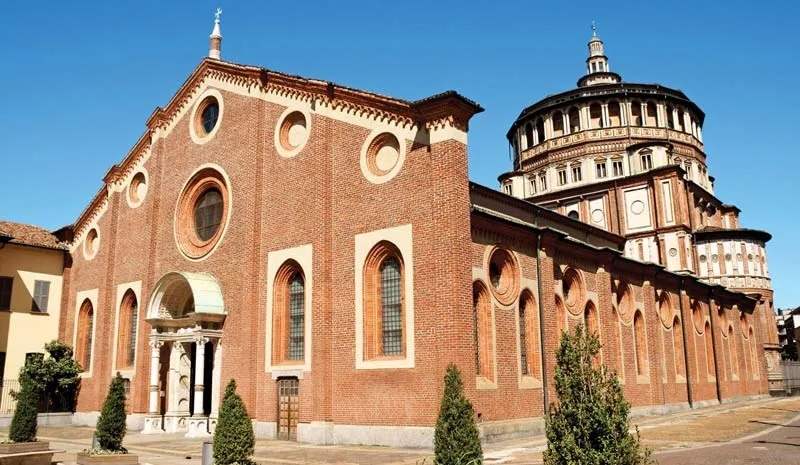
\includegraphics[scale=0.33]{img/churchmilan}
  \caption{米兰圣母玛丽亚感恩大教堂}
 \label{fig:church-Milan}
\end{figure}

塔尔塔利亚失去了布雷西亚的教授工作,他在贫穷和愤恨中走完了自己的一生。卡尔达诺的誓言似乎冥冥中笼罩着他。1560年他的长子被控毒杀不忠的妻子被判处死刑。卡尔达诺彻底被丧子之痛击倒了,他从米兰搬到布雷西亚住。1565年,卡尔达诺再次遭受打击,得意门生费拉里被他姐姐毒杀。卡尔丹诺沉迷赌博和占星术,他因推算出了耶稣的星象,被教会判处大逆不道,于1570年锒铛入狱。出狱后他移居罗马,在生命的最后一年出版了一本自传。在自传中,他不断重复丧子之痛,吹嘘自己的成就,但只用一句话轻描淡写地谈到了塔尔塔利亚。我们今天对这段历史的还原主要来自塔尔塔利亚的《新问题新发明》,以及他和中间人书商、卡尔达诺、费拉里往来的信件。

\begin{figure}[htbp]
 \centering
 \subcaptionbox{塔尔塔利亚\label{fig:tartaglia}}{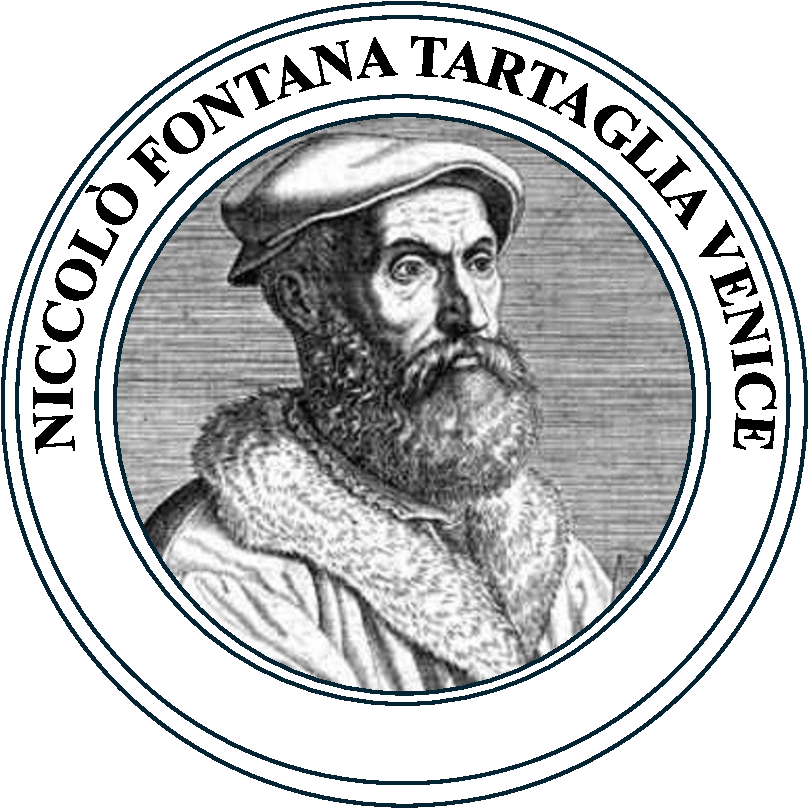
\includegraphics[scale=0.35]{img/tartaglia-coin}}
 \subcaptionbox{卡尔达诺\label{fig:cardano}}{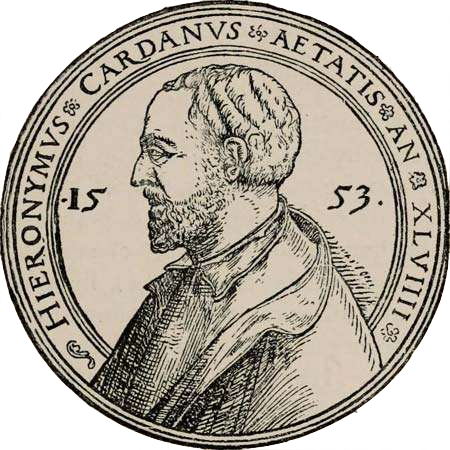
\includegraphics[scale=0.3]{img/Cardano}}
 \caption{塔尔塔利亚与卡尔达诺}
\end{figure}

今天,人们把三次方程的求根公式叫做卡尔达诺——塔尔塔利亚公式,简称卡尔达诺公式。此外塔尔塔利亚还在1546年发表过弹道学著作,第一个给出了弹道表格。1543年他第一个把欧几里得《原本》翻译成意大利语出版,此外他把阿基米德的一些著作翻译成意大利语。除了明显的缺陷外,卡尔达诺是一名百科全书式的学者。他是第一个对斑疹伤寒做出临床描述的人,数学上的贡献涵盖代数、概率论。他还发明了万向轴,被称作卡尔达诺轴。莱布尼茨评价到:“尽管有缺点,他是个伟人;但如果没有这些缺点,他将是无与伦比的。”

\section{三次方程}

与通常的观点不同,复数\underdot{不是}在解二次方程的过程中,而是在解三次方程的过程中被意外发现的。高中数学课上会给出卡尔达诺公式。本节将利用代数与几何两种方法推导这个公式。

\begin{figure}[htbp]
  \centering
  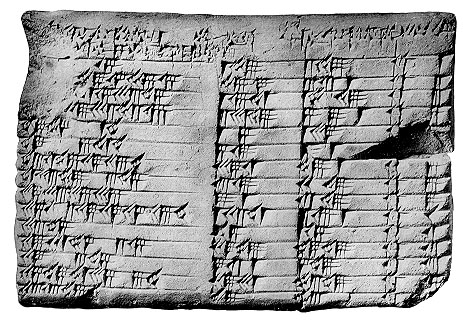
\includegraphics[scale=0.33]{img/plimpton322}
  \caption{编号普林普顿322的古巴比伦泥板,内容为勾股数表,约公元前2020年。藏于哥伦比亚大学。二十世纪二十年代由乔治·亚瑟、普林普顿捐赠给哥伦比亚大学。}
 \label{fig:plimpton322}
\end{figure}

%% https://personal.math.ubc.ca/~cass/courses/m446-03/pl322/pl322.html
我们是从古巴比伦泥板上了解到二次方程的早期历史的。如\cref{fig:plimpton322}所示,这是藏于哥伦比亚大学的一块泥板,编号为普林普顿322。这块泥板上的楔形文字内容很有特点,德国科学史家诺伊格鲍尔和萨克斯将发现它竟然是一张勾股数表。根据第1章给出的古巴比伦计数系统,我们很容易看出最后一列是编号$1, 2, 3, \dotsc, 15$,其中5,6,15三个数字损毁了。同样右边第二列也是编号。左边第二列的表头注明是直角三角形的底,从上到下转换为十进制依次是:$119, 3367, 4601, \dotsc, 1771, 56$,其中最后的56损毁了,并且有两处错误。左边第三列的表头注明是直角三角形的斜边,从上到下转换成十进制依次为:$169, 4825, 6649, \dotsc, 3229, 106$,同样最后的数字有错并且损毁了。左边第一列的数字最难破译,古巴比伦此时还没有使用零,也没有小数点。科学家们将其破译并转换为十进制数字,依次为:$1.9834\dotso, 1.94916\dotso, 1.9188\dotso$直到$1.43024\dotso, 1.38716\dotso$。60进制小数转换为10进制通常会除不尽(见\cref{thm:finite-decimal}),因此我们增加了省略号。如果我们记直角三角形的底为$w$,斜边为$d$,高为$h$,科学家们发现第一列的数字是$\dfrac{d^2}{h^2}$,根据勾股定理它等于$\dfrac{d^2}{d^2 - w^2}$。例如第一行:$d = 169, w = 119$,计算可得:

\[
\frac{d^2}{d^2 - w^2} = \frac{169^2}{169^2 - 119^2} = 1.9843\dotso
\]

%% https://engelsbergideas.com/notebook/the-brilliance-of-babylonian-mathematics/
正好是第一行中的第一个数字。这个勾股数表证实古巴比伦人知晓勾股定理(尽管没有定理的证明),并将其应用于计算。随着更多楔形文字泥板的出土,科学家们还发现了勾股定理的“配套练习题”。其中一道题目说:“已知长方形的面积和对角线,求长方形的两个边长。”这道典型的土地丈量问题相当于解方程:

\[
\begin{cases}
  ab = s \\
  a^2 + b^2 = d^2
\end{cases}
\]

其中$s$是面积,$d$是对角线。将$b = \dfrac{s}{a}$代入第二式,就得到关于$a^2$二次方程$(a^2)^2 - d^2 a^2 + s^2 = 0$。当时还没有代数符号系统,古巴比伦人解二次方程的过程是通过文字描述的。初中课堂上通常会在介绍求根公式前,学习用“配方法”(complete square)解二次方程。这本质上也是一种代数解法。阿拉伯数学家花拉子密在他的《代数学》中还遵循古希腊传统给出了二次方程的几何解释\footnote{即Hisab al-jabr w'al-muqabala,见第\ref{sec:Khwarizmi}节}。如果$a \ne 0$,我们可以把一般二次方程$ax^2 + bx + c = 0$的二次项系数化成1,然后把常数项移到右侧,得到$x^2 + \dfrac{b}{a}x = -\dfrac{c}{a}$。令$p = \dfrac{b}{a}, q= -\dfrac{c}{a}$,我们要通过几何方法解方程$x^2 + px = q$。如果$p > 0$,\cref{fig:quadratic1}给出了方程左侧的几何意义。$q$相当于一个正方形的面积$x^2$加上一个长$p$宽$x$的矩形面积。

\begin{figure}[htbp]
  \centering
  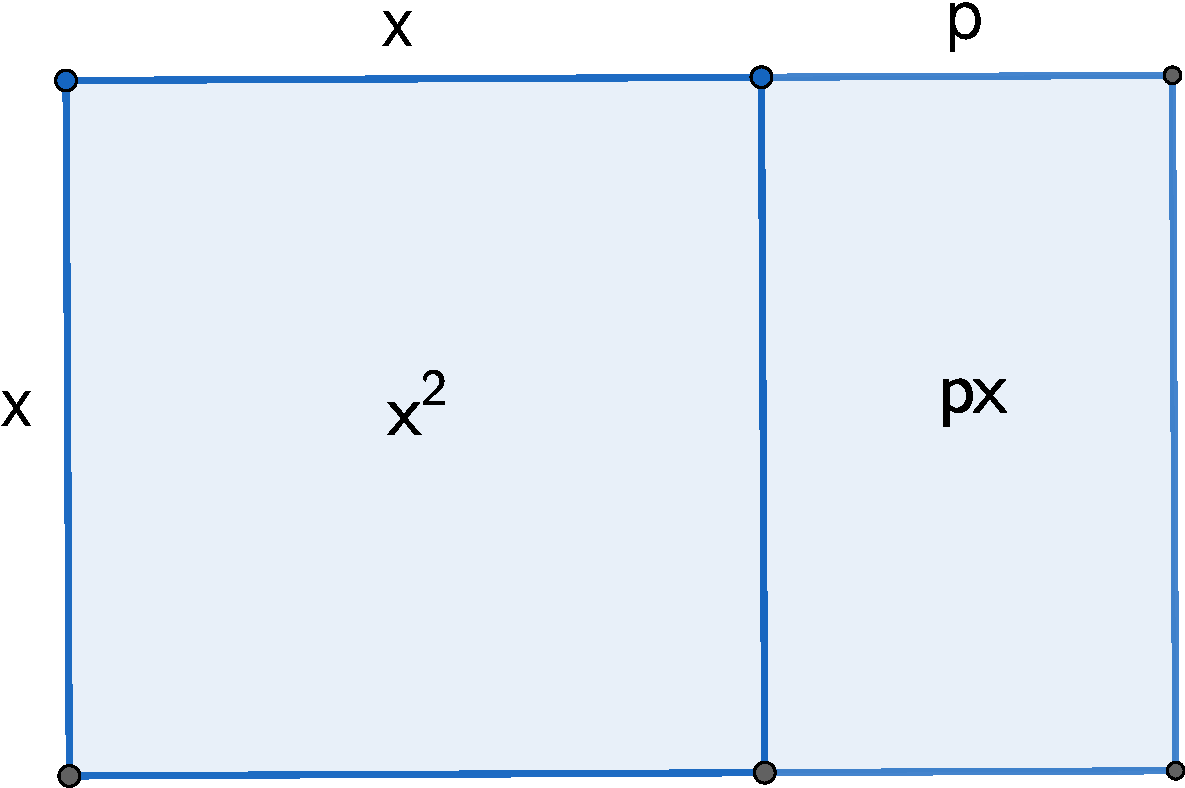
\includegraphics[scale=0.5]{img/quadratic1}
  \caption{$x^2 + px$的几何意义:正方形与长方形的面积和}
 \label{fig:quadratic1}
\end{figure}

配方法的几何意义是把矩形切分成两个同样的长$\dfrac{p}{2}$宽$x$的小矩形(见\cref{fig:quadratic2}左侧),然后把其中一个移动到正方形的下方,再补上一个边长为$\dfrac{p}{2}$的小正方形(见\cref{fig:quadratic2}右侧的黑色正方形)拼成一个边长为$x + \dfrac{p}{2}$的大正方形。左右两边图形中的白色面积相等,即:

\begin{align*}
 (x + \frac{p}{2})^2 &= q + (\frac{p}{2})^2 &&\text{大正方形面积等于白色部分加黑色部分} \\
 x + \frac{p}{2} &= \pm \sqrt{q + (\frac{p}{2})^2} &&\text{两边开方} \\
 x &= -\frac{p}{2} \pm \sqrt{q + \frac{p^2}{4}} \\
 x &= -\frac{b}{2a} \pm \sqrt{-\frac{c}{a} + \frac{b^2}{4a^2}} &&\text{代入}p = \frac{b}{a}, q= -\frac{c}{a} \\
 x &= \frac{-b \pm \sqrt{b^2 - 4ac}}{2a}
\end{align*}

\begin{figure}[htbp]
  \centering
  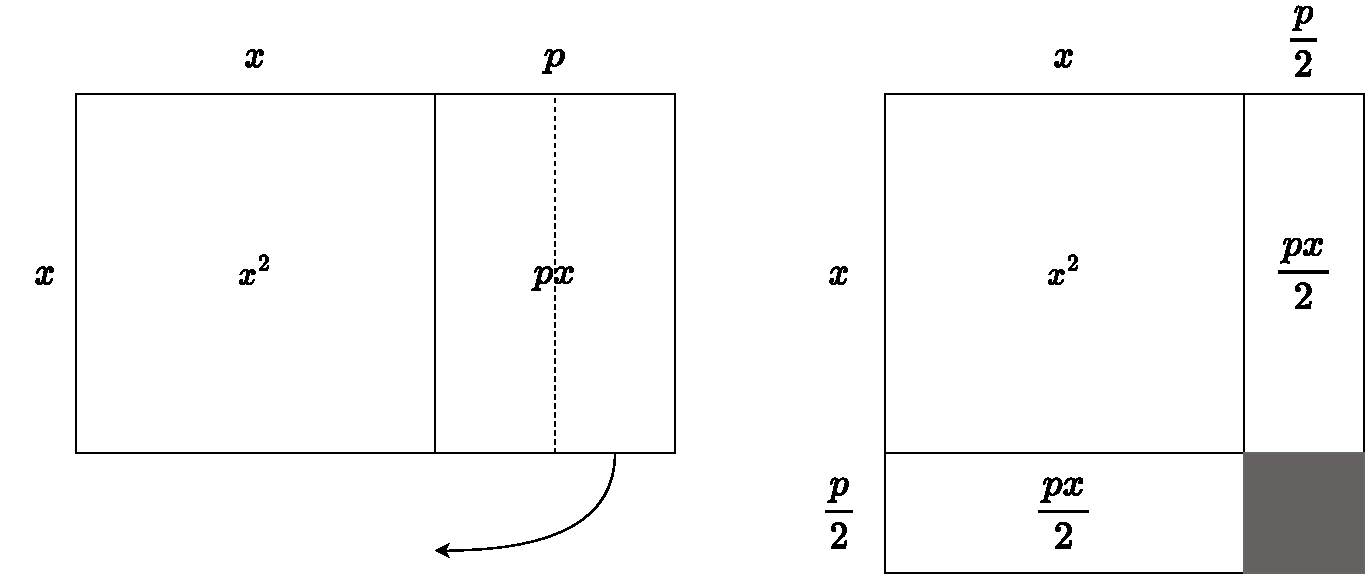
\includegraphics[scale=0.5]{img/quadratic2}
  \caption{$x^2 + px$的几何意义:正方形与长方形的面积和}
 \label{fig:quadratic2}
\end{figure}

这就是常见的一元二次方程求根公式。但在花拉子密时代负数还没有被接受,因此当一次项为负时就需要给出$x^2 - px = q$的几何解释;当常数项为负时需要给出$x^2 - q = px$的几何解释(见\cref{qn:geometric-quadratic})。卡尔达诺在《大术》中遵循了这样的传统,同时给出了三次方程的代数解法和几何解释。我们先介绍代数解法。对于一般三次方程$a_3x^3 + a_2x^2 + a_1x + a_0 = 0, a_3 \ne 0$,首先两边同时除以$a_3$把三次项系数化为1,即$x^3 + \dfrac{a_2}{a_3} x^2 + \dfrac{a_1}{a_3} x + \dfrac{a_0}{a_3}$。重新命名系数为$x^3 + ax^2 + bx + c = 0$。大约在十四世纪末,意大利佛罗伦萨的数学家就发现可以通过变量替换$x = y - \dfrac{a}{3}$把二次项消去:

\begin{align*}
(y - \frac{a}{3})^3 + a(y - \frac{a}{3})^2 + b(y - \frac{a}{3}) + c &= 0  \\
y^3 -\cancel{ay^2} + \frac{a^2}{3}y - \frac{a^3}{27} + \cancel{ay^2} - \frac{2a^2}{3}y + \frac{a^3}{9} + by - \frac{ab}{3} + c &= 0 && \text{二项式展开} \\
y^3 + (b - \frac{a^2}{3})y + \frac{2a^3}{27} - \frac{ab}{3} + c &= 0 \\
y^3 + py + q = 0
\end{align*}

其中$p = b - \dfrac{a^2}{3}, q = c + \dfrac{2a^2}{27} - \dfrac{ab}{3}$。由于当时人们不接受负数,根据$p, q$的正负,这种“缺二次项”的三次方程共有三种形式:

\begin{align}
y^3 + py &= q \label{eq:cubic-linear} \\
     y^3 &= py + q \label{eq:cubic-complex} \\
y^3 + q &= py
\end{align}

其中费罗独立发现的是\cref{eq:cubic-linear}形式的解,而\cref{eq:cubic-complex}形式的解直接导致了复数的发现。我们不妨以$y^3 = py + q$为例继续推导求根公式。令$y = u + v$,则方程左侧化为:

\begin{align*}
y^3 = (u + v)^3 &= u^3 + 3u^2v + 3uv^2 + v^3 && \text{二项式展开} \\
  &= u^3 + v^3 + 3uv(u + v) \\
  &= u^3 + v^3 + 3uvy && \text{代入} y = u + v \\
  &= (3uv)y + (u^3 + v^3) = py + q && \text{左边等于右边}
\end{align*}

由待定系数法知:

\[
\begin{cases}
  3uv = p \\
  u^3 + v^3 = q
\end{cases}
\]

这相当于关于$u, v$的二元方程组。从第一个方程中得到:$v = \dfrac{p}{3u}$,代入第二个方程得:

\[
u^3 + (\frac{p}{3u})^3 = q
\]

这实际上是一个关于$u^3$的二次方程:$(u^3)^2 - qu^3 + (\dfrac{p}{3})^3 = 0$,利用二次方程求根公式得到:

\[
u^3 = \frac{q}{2} \pm \sqrt{(\frac{q}{2})^2 - (\frac{p}{3})^3}
\]

注意到$u, v$在上面的二元方程组中是完全对称的,$v^3$必然具有同样的形式。我们不妨让它们分别取这两个根:

\[
\begin{cases}
u^3 = \dfrac{q}{2} + \sqrt{(\dfrac{q}{2})^2 - (\dfrac{p}{3})^3} \\
v^3 = \dfrac{q}{2} - \sqrt{(\dfrac{q}{2})^2 - (\dfrac{p}{3})^3}
\end{cases}
\]

这样它们满足$u^3 + v^3 = q$。最后由$y = u + v$,我们得到方程的根:

\be \label{eq:cardano}
y = u + v = \sqrt[3]{\frac{q}{2} + \sqrt{(\frac{q}{2})^2 - (\frac{p}{3})^3}} + \sqrt[3]{\frac{q}{2} - \sqrt{(\frac{q}{2})^2 - (\frac{p}{3})^3}}
\ee

这就是高中数学课上介绍的卡尔达诺公式。我们进一步可以用$x = y - \dfrac{a}{3}$求出未知数$x$。与此对照,我们接下来用几何法解三次方程$y^3 + py = q$。如\cref{fig:cube-decompose}所示,把一个边长为$r$的大正方体切分为5部分:左前下角的边长为$r-s$的小正方体;右后上角的边长为$s$的小正方体;三个长$r$宽$r-s$高$s$的长方体,分别位于左上、右前、后下。大正方体的体积等于这5部分的体积之和,即:

\begin{figure}[htbp]
  \centering
  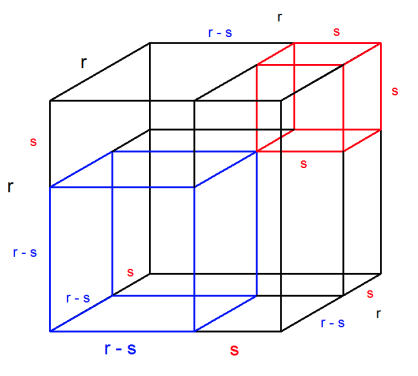
\includegraphics[scale=0.4]{img/cube-decompose}
  \caption{把边长为$r$的正方体切分成5部分}
 \label{fig:cube-decompose}
\end{figure}

\begin{align*}
r^3 = (r-s)^3 + s^3 + 3rs(r-s)  &&\text{两个正方体加三个长方体} \\
(r-s)^3 + 3rs(r-s) = r^3 - s^3
\end{align*}

令$p = 3rs, q = r^3 - s^3$,则上述等式就是$(r-s)^3 + p(r-s) = q$。显然$y = r - s$就是方程$y^3 + py = q$的一个解。所以只要根据$p, q$找到合适$r, s$就能解出三次方程了。由$p = 3rs$得$s = \dfrac{p}{3r}$,代入$q = r^3 - s^3$得到方程:

\[
r^3 - (\frac{p}{3r})^3 = q
\]

这本质上是一个关于$r^3$的二次方程$(r^3)^2 - qr^3 - (\dfrac{p}{3})^3 = 0$,利用二次方程求根公式得到:

\[
r^3 = \frac{q}{2} + \sqrt{(\frac{q}{2})^2 + (\frac{p}{3})^3}
\]

对称地可以求出$s^3$:

\[
s = -\frac{q}{2} + \sqrt{(\dfrac{q}{2})^2 + (\dfrac{p}{3})^3}
\]

最终求得未知数$y = r - s$:

\[
y = r - s = \sqrt[3]{\frac{q}{2} + \sqrt{(\frac{q}{2})^2 + (\frac{p}{3})^3}} - \sqrt[3]{\frac{q}{2} + \sqrt{(\frac{q}{2})^2 + (\frac{p}{3})^3}}
\]

和代数法推出的卡尔达诺公\cref{eq:cardano}对比,只有$p$的正负号不同,这是由于方程$y^3 + py = q$和$y^3 = py + q$中$p$的符号相反。我们可以尝试用卡尔达诺公式解方程$x^3 = 6x + 9$。

\begin{align*}
x &= \sqrt[3]{\frac{9}{2} + \sqrt{(\frac{9}{2})^2 - (\frac{6}{3})^3}} + \sqrt[3]{\frac{9}{2} - \sqrt{(\frac{9}{2})^2 - (\frac{6}{3})^3}} \\
  &= \sqrt[3]{\frac{9}{2} + \sqrt{\frac{81 - 32}{4}}} + \sqrt[3]{\frac{9}{2} - \sqrt{\frac{81 - 32}{4}}} \\
  &= \sqrt[3]{\frac{9}{2} + \frac{7}{2}} + \sqrt[3]{\frac{9}{2} - \frac{7}{2}} \\
  &= \sqrt[3]{8} + \sqrt[3]{1} = 2 + 1 = 3
\end{align*}

验证的确有$3^3 = 27 = 6 \times 3 + 9$。三次方程的公式解是数学上的重大突破,人们迫不及待地用它来解决各种个样的问题。可是有些方程的结果却令人大惑不解,其中最著名的例子是方程$x^3 = 15x + 4$。通过观察$x = 4$是方程的一个解:$4^3= 64 = 60 + 4 = 15 \times 4 + 4$。但卡尔达诺公式给出的结果是:

\begin{align*}
x &= \sqrt[3]{2 + \sqrt{2^2 - 5^3}} + \sqrt[3]{2 - \sqrt{2^2 - 5^3}}  \\
  &= \sqrt[3]{2 + \sqrt{-121}} + \sqrt[3]{2 - \sqrt{-121}}
\end{align*}

\index{数学家!邦贝利}
竟然在二次根号下出现了负数。以前在解二次方程时,如果判别式的值为负,人们可以说“无解”。但这个方程明明有一个解$x = 4$,并非“无解”。人们必须正视这个问题。卡尔达诺不知道如何解答,他在《大术》中评论道:“这些数即微妙又无用。”在这个问题上取得突破的是意大利数学家邦贝利(Rafael Bombelli, 1526~1572)。邦贝利设想把$\sqrt[3]{2 \pm \sqrt{-121}}$化简成$a \pm b\sqrt{-1}$的形式。这样卡尔达诺公式的两项加起来就是:

\[
\sqrt[3]{2 + \sqrt{-121}} + \sqrt[3]{2 - \sqrt{-121}} = a + b\sqrt{-1} + a - b\sqrt{-1} = 2a = 4
\]

这样就确定出$a = 2$。接下来通过待定系数法确定$b$的值。邦贝利假设$(\sqrt{-1})^2 = -1$,把两边乘3次方:

\begin{align*}
2 + \sqrt{-121} &= (2 + b\sqrt{-1})^3 \\
  &= 8 + 12b\sqrt{-1} - 6b^2 - b^3\sqrt{-1} && \text{二项式展开} \\
  &= (8 - 6b^2) + (12b - b^3)\sqrt{-1}
\end{align*}

由$2 = 8 - 6b^2$得出$b = \pm 1$;把1代入$(12b - b^3)\sqrt{-1}$得$11\sqrt{-1}$。平方后可验证:$(11\sqrt{-1})^2 = -121$。于是有$\sqrt[3]{2 + \sqrt{-121}} = 2 + \sqrt{-1}$。对于$b = -1$,邦贝利接着通过两边乘3次方验证了$\sqrt[3]{2 - \sqrt{-121}} = 2 - \sqrt{-1}$也成立。他对这个结果非常满意,在1572年出版的《代数》一书中写道:“起初,我感到这样处理更像是诡辩而非真理,但我不断探寻,直至找到证明。”\cite{OMerino-2006}邦贝利的数学观点远远超越了他的时代。当时负数尚未被欧洲接受,邦贝利在《代数》中不仅正确地定义了正负数之间的运算规则,还给出了复数的计算规则。他称$\sqrt{-n}$为“负的正”(plus of minus)称$-\sqrt{-n}$为“负的负”(minus of minus),然后写道\cite{MacTour-Bombelli}:

\begin{quotation}
负的正乘以负的正为负,即:$\sqrt{-n} \times \sqrt{-n} = -n$;

负的正乘以负的负为正,即:$\sqrt{-n} \times -\sqrt{-n} = n$;

负的负乘以负的正为正,即:$-\sqrt{-n} \times \sqrt{-n} = n$;

负的负乘以负的正为负,即:$-\sqrt{-n} \times -\sqrt{-n} = -n$;
\end{quotation}

非常遗憾的是,邦贝利原来准备出版五卷本《代数》,但1572年出版了前三卷后他就去世了。剩余的两卷本草稿直到1923年才被发现于意大利博洛尼亚的图书馆。当时的人们并没有相信并接受邦贝利的观点,数学界基本排斥$\sqrt{-1}$。在接下来的200年间,即使有少数学者如沃利斯尝试赋予复数涵义,但大多数人要么怀疑,要么忽视了邦贝利的计算规则。直到1770年,大数学家欧拉仍然在他的著作中“证明”$\sqrt{-2} \times \sqrt{-3} = \sqrt{6}$,我们今天看到这个结论会感到很意外\footnote{欧拉实际上用符号$\sqrt{6}$表示6的一对平方根$\pm\sqrt{6}$,类似地$\sqrt{-2}$表示-2的一对平方根$\pm\sqrt{-2}$,$\sqrt{-3}$表示-3的一对平方根$\pm\sqrt{-3}$,这样欧拉的本意是想表示$\pm \sqrt{-2} \times \pm \sqrt{-3} = \pm \sqrt{6}$的所有组合}。也有人高度评价邦贝利的工作,莱布尼茨说他是“杰出的分析艺术大师。”今天人们称邦贝利为“虚数之父”。

\begin{figure}[htbp]
  \centering
  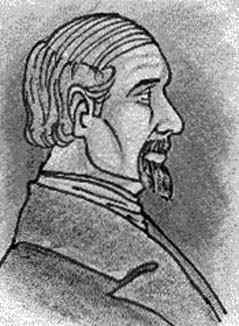
\includegraphics[scale=0.4]{img/Bombelli}
  \caption{拉斐尔·邦贝利,1526~1572}
 \label{fig:Bombelli}
\end{figure}

邦贝利的方法中使用了$a + b\sqrt{-1}$的形式。第一个使用$a + \sqrt{-b}$的是卡尔达诺,但是他否定了自己的结论。在《大术》第37章,卡尔达诺给出了这样的一个问题:把10分成两部分,使得它们的乘积是40。列方程就是:

\[
\begin{cases}
x + y = 10 \\
xy = 40
\end{cases}
\]

消元可得一元二次方程$x(x-10) = 40$。我们知道,把10分成两部分最大的乘积是$5 \times 5 = 25$,所以乘积40是不可能的(也可以这样思考:把一根长20厘米的绳子围成矩形,面积最大时是边长为5的正方形,此时面积是25平方厘米)。卡尔达诺写道:

\begin{quotation}
显然这是不可能的。尽管如此,我们可以这样做:我们把10均分成两个5,平方是25。减去40,如果你希望的话,得-15。把-15的平方根加上、减去5得到的两个数的乘积就是40。因此这两个数是$5 + \sqrt{-15}$和$5 - \sqrt{-15}$。

尽管匪夷所思,把两个数$5 + \sqrt{-15}$和$5 - \sqrt{-15}$相乘得$25-(-15)$,因此它们的积是40。
\end{quotation}

卡尔达诺的方法是把10分成$5 + x$和$5 - x$,让它们的积是40。利用平方差公式$(5 + x)(5 - x) = 25 - x^2 = 40$,因此$x^2 = -15$。这样推出解为$x_{1, 2} = 5 \pm \sqrt{-15}$。正是由于其在现实应用,特别是在一元二次方程应用中的不合理性,卡尔达诺以及同时代的大多数人舍弃了复数答案。但是邦贝利意识到在三次方程的\underdot{合理}应用中,作为中间结果的复数有其存在价值。那么“虚数”这个名字是怎么来的呢?这要“归功”于笛卡尔。笛卡尔在1637年发表的《谈谈方法》的附录《几何学》中创建了解析几何。方程的根对应曲线间的交点或曲线与坐标轴的零点。尽管当时人们没有认识到代数基本定理,笛卡尔还是敏锐地洞见到方程根的个数等于方程的次数。但是从几何上的观点上看,某些曲线不和$x$轴相交,或者曲线间不相交。面对这些几何上不可能的构造,笛卡尔认为它们的交点或零点是虚构的。“虚数”一词就来自笛卡尔文中的imaginary,在英文中它同时还有想象的涵义。笛卡尔写道:“对于任何方程,人们可以想象(imagine)有着和次数同样多的根,但在很多情况下,这些根对应的值并不存在。”

我们今天广泛使用符号$i$作为虚数单位。这个符号是欧拉选定的。它是imaginary的首字母。笛卡尔的态度反映了当时大多数人的观点。数学家们并不喜欢虚构、想象这些涵义。其中一个原因是$\sqrt{-n}$带来了混乱和歧义。例如常见的运算规则$\sqrt{ab} = \sqrt{a}\sqrt{b}$还成立么?有人指出这样的问题:

\begin{align*}
70 &= \sqrt{4900} = \sqrt{(-100)\times(-49)} = \sqrt{-100}\sqrt{-49} \\
   &= (10i)(7i) = 70 \times (-1) = -70
\end{align*}

这样就出现了$70 = -70$的矛盾结论(见\cref{qn:sqrt-of-product})。复变函数之父柯西建议拒绝符号$\sqrt{-1}$,高斯对$i$也不满意,建议取个新名字。但他的建议太晚了,$i$已经被广泛使用,直到今天。

\section{佚名数学家}

为了让复数真正进入数的大家族得到承认,必须解决它的意义问题。并且这种意义不能是牵强附会的空中楼阁,它必须是自然的、让人信服的并且能解决真正的问题。1673年,微积分的先驱者英国数学家沃利斯试图给出复数的几何解释,但是他和成功失之交臂。沃利斯是数轴的发明者,他正是利用数轴作为武器,尝试解方程$x^2 + 2bx + c^2 = 0$。根据二次方程求根公式,方程的两个根是:$x_{1,2} = -b \pm \sqrt{b^2 - c^2}$。如\cref{fig:wallis1}所示,沃利斯在数轴上找到$-b$,然后以这点为垂足构造一左一右两个直角三角形,其高为$c$、斜边为长$b$。根据勾股定理,另一直角边长为$a = \sqrt{b^2 - c^2}$。所以点$-b$左右两侧距离$a$的两个点就是$x_{1,2}$。

\begin{figure}[htbp]
  \centering
  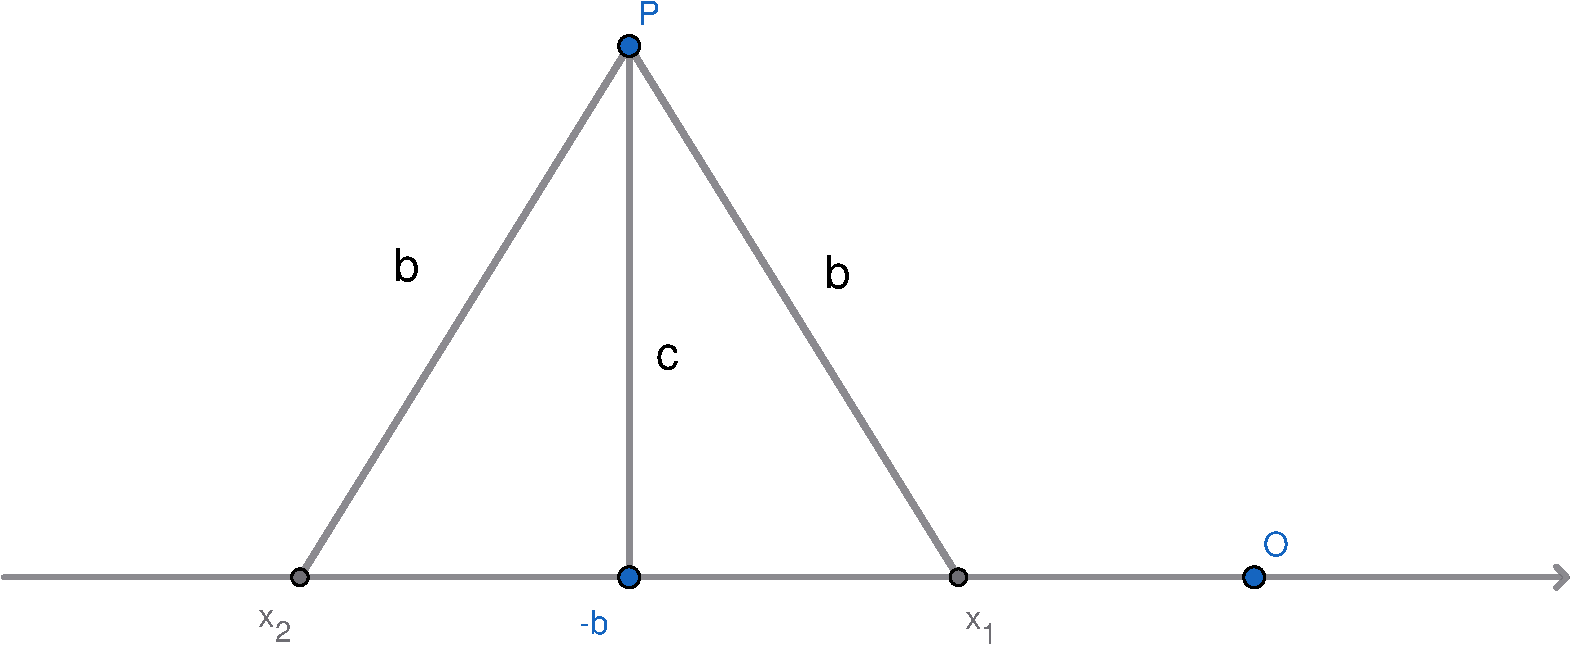
\includegraphics[scale=0.33]{img/wallis1}
  \caption{根$x_{1,2} = -b \pm \sqrt{b^2 - c^2}$在数轴上的位置}
 \label{fig:wallis1}
\end{figure}

到此为止一切正常。接着沃利斯不断增大$c$的值,两个根$x_{1,2}$越来越靠近$-b$点。当$c = b$时两个根重合了。如果继续增大$c$会怎样呢?沃利斯绘制出了这样一幅图,如\cref{fig:wallis2}所示。

\begin{figure}[htbp]
  \centering
  \subcaptionbox{沃利斯认为$-b \pm i\sqrt{c^2-b^2}$所在的位置\label{fig:wallis2}}{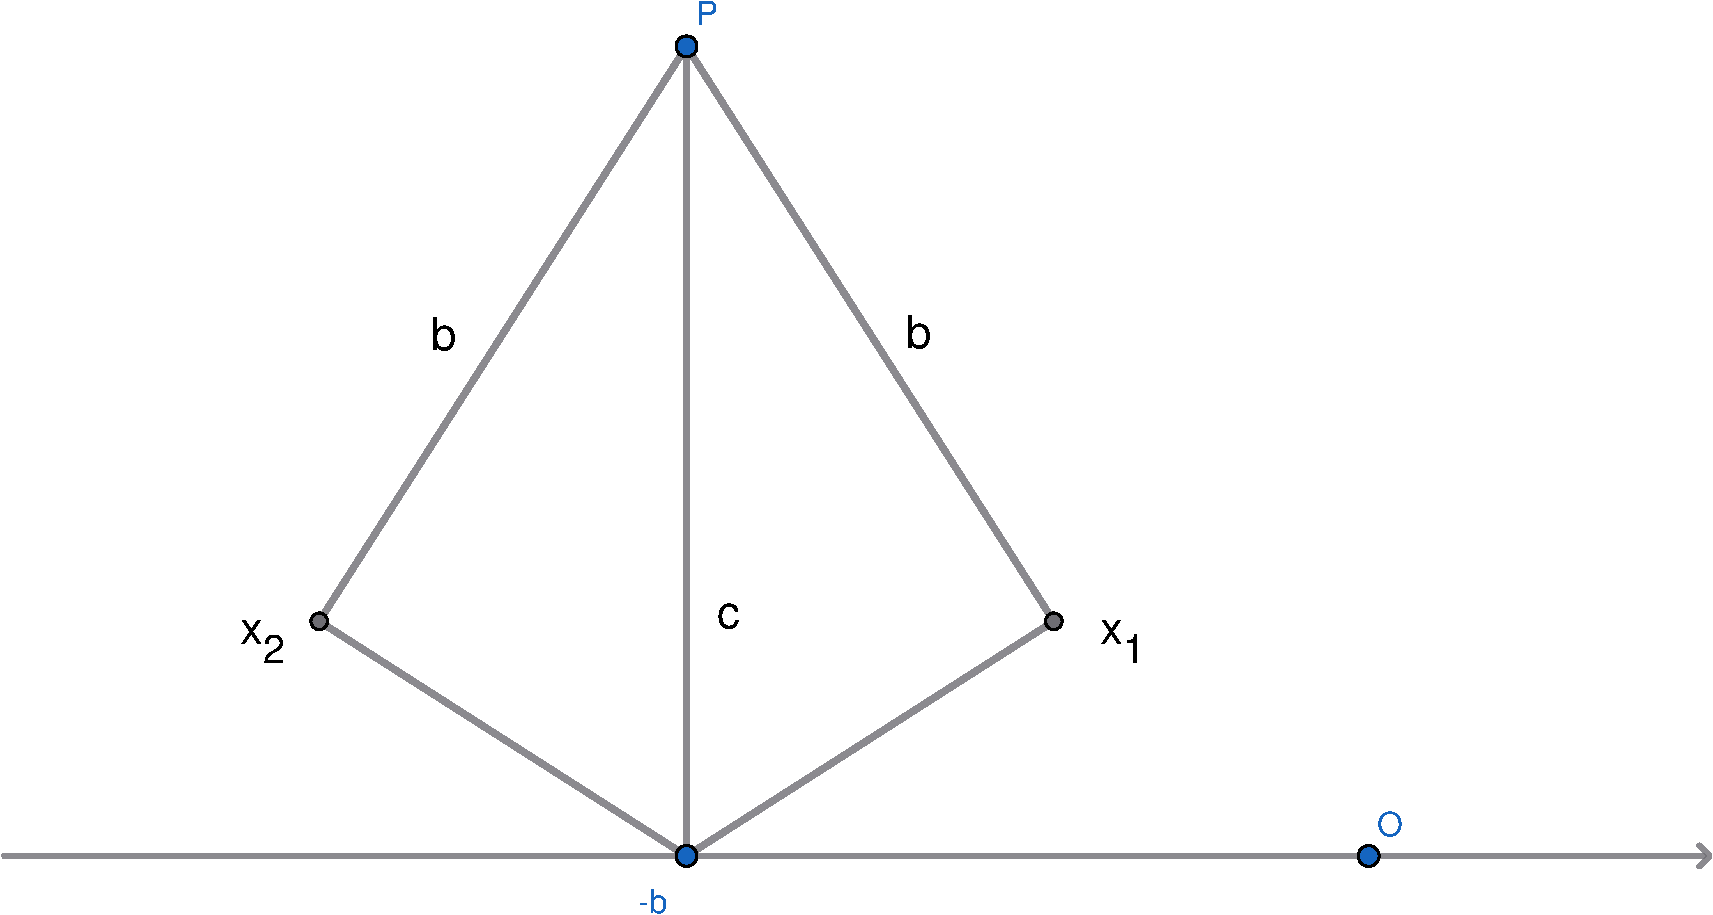
\includegraphics[scale=0.33]{img/wallis2}}
  \subcaptionbox{实际上$-b \pm i\sqrt{c^2-b^2}$在复平面上的位置\label{fig:wallis3}}{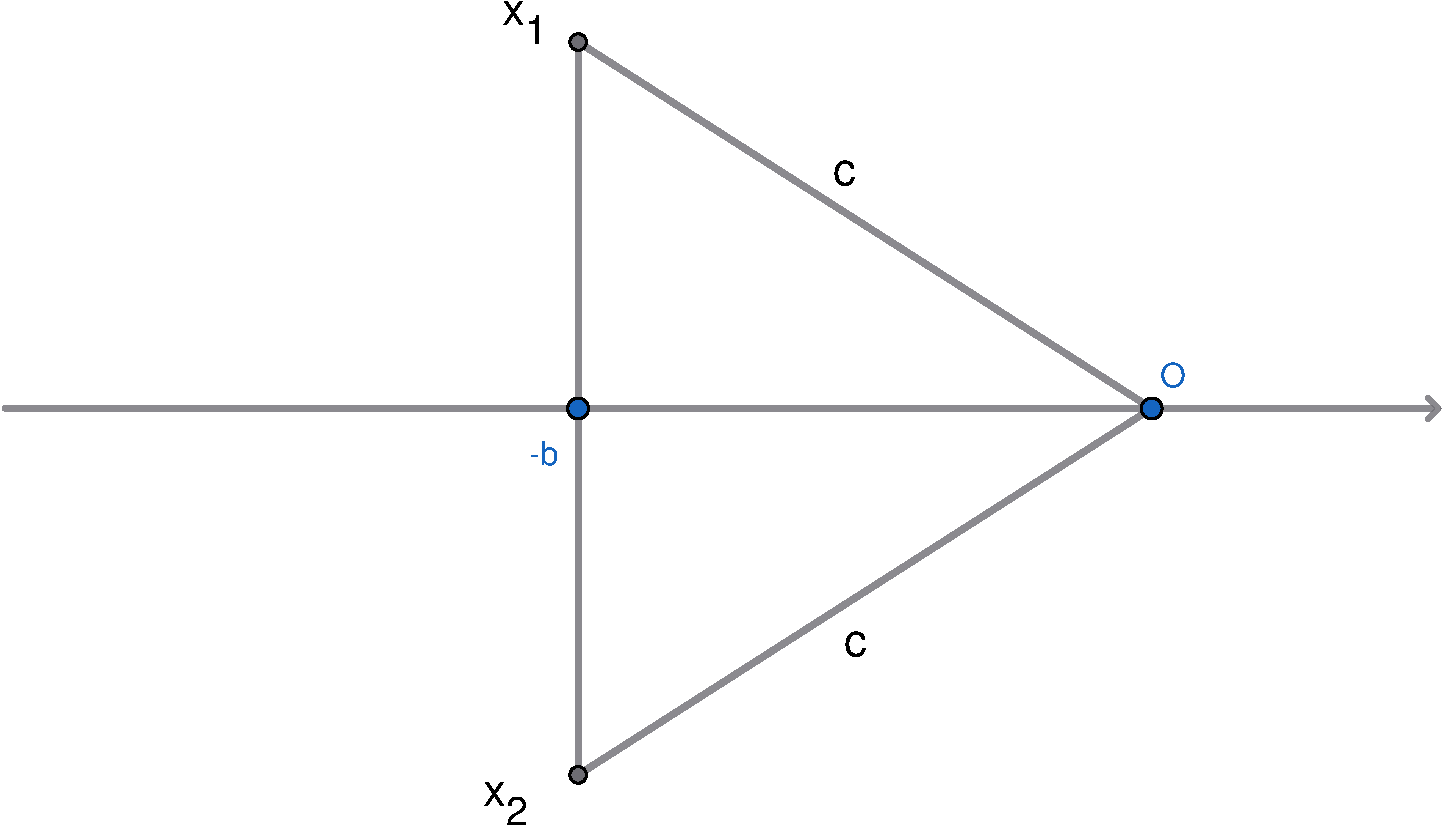
\includegraphics[scale=0.33]{img/wallis3}}
  \caption{方程$x^2 + 2bx + c^2 = 0$的两个根}
\end{figure}

\index{数学家!韦塞尔}
这已经非常接近真相了。沃利斯认为此时$c$成为斜边,一条直角边是$b$,另一直角边是$\sqrt{c^2 - b^2}$,但它们仍然在点$-b$的左右两侧。实际上沃利斯只要把左右两侧换成上下就能触摸到复平面了。这真令人惋惜。在历史上第一成功解决了复数几何意义的人是丹麦-挪威数学家卡斯帕尔·韦塞尔(Caspar Wessel,1745~1818)。1797年3月10日,韦塞尔向丹麦皇家科学提交了他的著作,题为《论方向的解析表示——主要应用于平面和球面多边形求解的尝试》。他成功地把复数$a + bi$表示为平面直角坐标系中从原点指向坐标$(a, b)$的线段(即向量),并且定义了向量间的代数计算规则,包括加法和乘法。从几何的角度,加法规则相当于“平行四边形”原理;乘法相当于把线段的长度相乘,然后把各自相对于横轴的角度相加。韦塞尔的论文于两年后发表。非常遗憾的是,韦塞尔的职业是一名测量员而非知名数学家,并且论文的语言是丹麦语,当时并未引起广泛的关注。韦塞尔的名字被大多数人忽略了,直到约100年后的1895年,他的工作才重新引起人们重视。挪威数学家索菲斯·李重新发表了韦塞尔的论文。更加匪夷所思的是,1806年,一个年轻人重新独立发现了复平面和复数的几何意义,但没有人知道他的名字。

\subsection{佚名作者阿尔冈}
\index{数学家!阿尔冈}
1806年金秋,一位年轻人敲开了法国科学院院士数学家勒让德家的大门。他十分紧张,勒让德被认为是欧拉最好的弟子,拉格朗日的接班人。拿破仑重建科学院后,任命勒让德为数学部的负责人,法国最高学府巴黎综合工科学校的主考官。这位年轻人做了简单的自我介绍,由于紧张,他甚至忘记了介绍自己的名字。他恭敬地把自己的一篇研究手稿交给了勒让德,恳请他指正。年轻人没有仔细向勒让德解释他的目的,但是当被问起论文的内容时,他立刻兴奋起来了。“哦,尊敬的院士先生”,年轻人说:“这是一篇关于虚数的研究工作,我发现虚数其实是有意义的,它就像其它的数那样真实!只要我们把它们看成是线段,就会发现……”面对滔滔不绝的年轻人,勒让德一脸狐疑。他只好打断了这个年轻人。“我现在很忙,不过我答应有时间读一读你的文章,我们今天先到这里吧。”在大门关闭前年轻人再次恳请勒让德:“院士先生,我非常期待您的批评指正。”

送走了这位年轻人,勒让德很快就忙于其它研究和科学院的事务了。直到几周后,勒让德偶然看到了放在案头的几张纸,题目是《关于在几何构造中表示虚数的一种方法的论述》。这是谁送来的?哦,想起来了,那个年轻人叫什么来着?好像记不清了,不管怎样,勒让德读了下去。出乎意料的是,勒让德一旦开始读就立刻被这篇文章吸引住了。绝对出人意料的创新想法,行云流水般的论述,扎实的计算,精确的结论,把数、几何、三角函数完美地结合在一起。勒让德决定马上联系一下这位小伙子,和他深入讨论。可他翻遍了论文的前前后后,也没有找到任何姓名、地址。怎么会这样呢?也许这位年轻人过两天会再次登门拜访吧?勒让德决定等一等。一天、两天……从深秋等到初冬,转眼巴黎已经飘下了第一场雪。可年轻人再也没有出现。这位年轻人会不会直接在期刊上发表他的论文?这样我就能找到他讨论了。勒让德跑到图书馆检查了过去几个月的各种数学期刊,但再次让他失望。也许当天勒让德的态度让这位年轻人心灰意冷,放弃了这个研究。11月2日,勒让德把这篇论文寄给了他的朋友与合作者数学家弗朗索瓦·弗朗塞,并附上了一小段评论,他称赞了那位不慕虚荣热爱学术的年轻人,并认为尽管是草稿,但是具有足够的创新性。

弗朗索瓦·弗朗塞主要研究偏微分方程,尽管他的工作经常得到法国科学院的赞誉,但很少在生前发表。1810年弗朗塞死后,他的兄弟雅克·弗朗塞在整理遗稿时发现了这篇关于复数的论文,并于1813年9月以题目《新的位置几何学原理及虚数符号的解释》发表。雅克·弗朗塞展示了一个真正学者的风范,他没有把这个成果据为己有。在论文的结尾他指出这些想法来自一位不知名的数学家,并恳请这位数学家站出来以得到应有的荣誉。雅克·弗朗塞的这篇论文发表在热尔岗的著名期刊《数学年鉴》上不久,一位名叫阿尔冈的人来信声称他就是那位不知名的作者,并寄来了一份稍加修改的原稿,题目正是《关于在几何构造中表示虚数的一种方法的论述》。阿尔冈在其中加入了新的应用。这件本来就充满戏剧性的事件接下来引起了众多数学家的关注:雅克·弗朗塞、阿尔冈和数学家塞尔瓦在《数学年鉴》上展开了激烈的讨论。塞尔瓦认为必须用纯代数来处理复数,而雅克·弗朗塞和阿尔冈则主张几何表示法的有效性。阿尔冈接下来展示了复数几何表示法的威力——他一举证明了代数基本定理。以今天的眼光看,尽管有些瑕疵,但这是诸多证明中最清晰优美的一个。阿尔冈的工作是化时代的,但非常遗憾的是,我们不知道他究竟是谁!他在所有的论文中都仅仅署名“阿尔冈”。西方人的姓名是名字加姓氏,有的还有中间名。因此这相当于中国人仅仅署名“张”,究竟是张什么却一无所知。究竟是众多姓阿尔冈的人中的哪一位啊?我们只知道他1806年出现在巴黎,1813年发表的论文是从巴黎寄出的。有人猜测是他可能是让·罗伯特·阿尔冈,一位住在巴黎的会计员和业余数学家,但年龄对不上。1806年,勒让德描述的是一位年轻人,但彼时的让·罗伯特·阿尔冈已经38岁了\cite{MacTour-Argand}。

\index{阿尔冈图}
我们对这段历史的复原主要来自勒让德写给弗朗索瓦·佛朗塞的信,以及雅克·弗朗塞的论文。为了纪念阿尔冈的成就,今天我们把\cref{fig:Argand-diagram}叫做“阿尔冈图”(Argand diagram),它出现在全世界所有的中学课堂上\cite{Weisstein-2025}。

\begin{figure}[htbp]
  \centering
  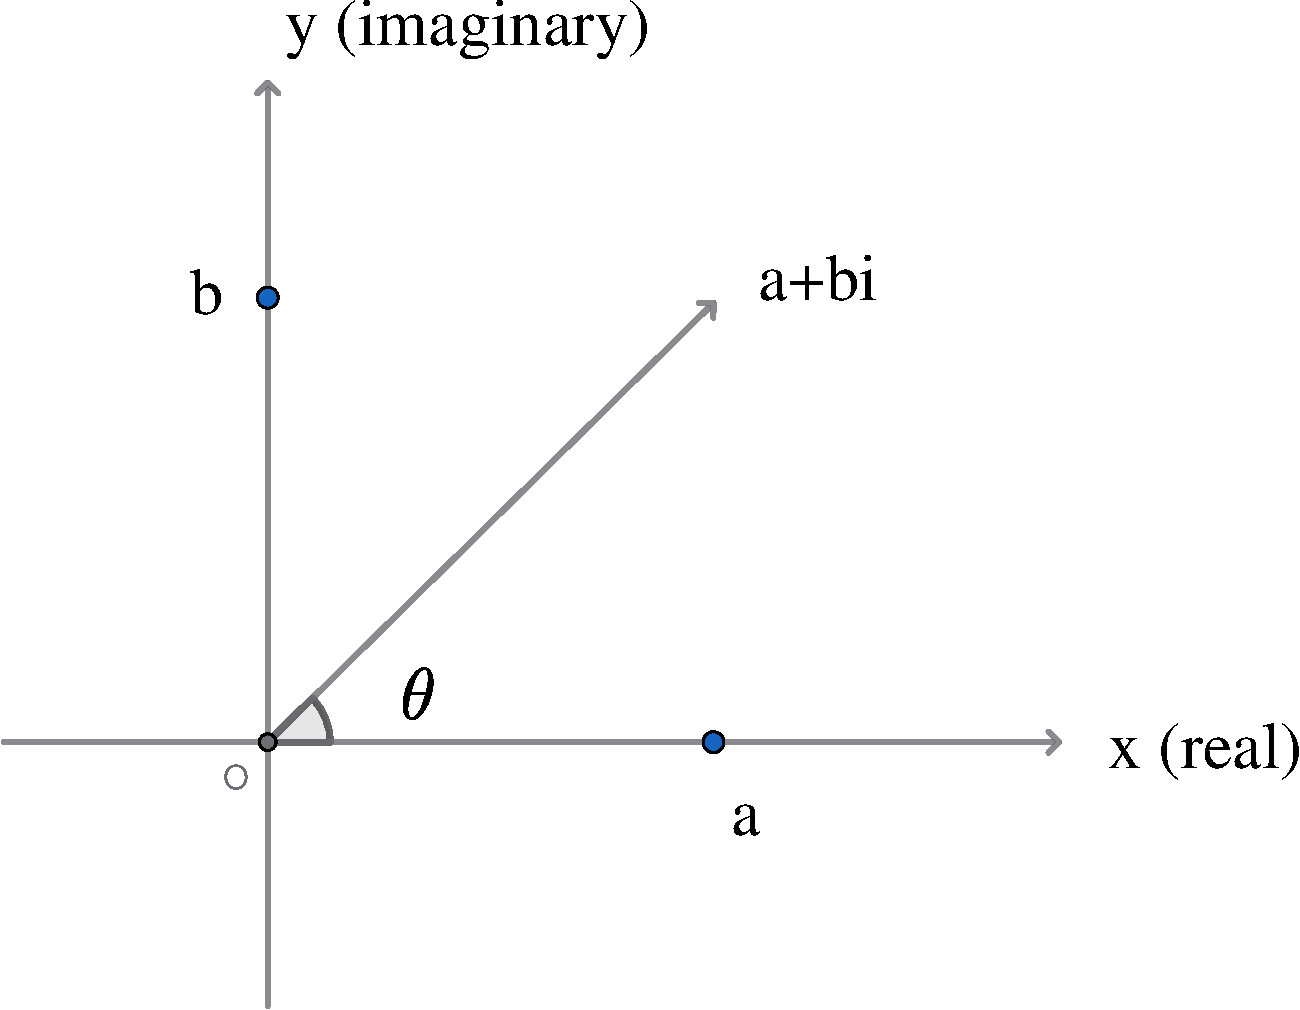
\includegraphics[scale=0.33]{img/argand-diagram}
  \caption{阿尔冈图}
 \label{fig:Argand-diagram}
\end{figure}

\subsection{复数的几何意义}

一图胜千言。我们可以立刻从阿尔冈图上看到复数$z$包含两个部分:实部$a$和虚部$bi$。虚轴创造性地垂直向上,实轴和虚轴彼此垂直,张成了复平面。复数被表示成了一个\underdot{向量},从原点指向复平面上坐标为$(a, b)$的点。画成一个带有箭头的线段,这个向量就是$a + bi$。虚数单位$i$不是任何实数,因为它根本不在实轴上。如果说实数轴上的任何数$a$乘以$-1$相当于“向后转”,变成指向另一侧的负数$-a$,那么$a$乘以$i$相当于“向左转$90\degree$”,变成虚轴上的$ai$;再次乘以$i$相当于再次“向左转$90\degree$”,变回实数轴上指向另一侧的$-a$。两次转$90\degree$相当于转$180\degree$,这就完美地解释了$i^2 = -1$。我们由勾股定理立刻看出向量$a + bi$所代表的线段的长度是$r = \sqrt{a^2 + b^2}$,它叫做复数$z$的模(modulus),记做$|z|$。向量与实轴张角为$\theta$,叫做复数的幅角(argument),记做$arg(z)$。由三角函数的定义我们立刻知道复数的实部与虚部可以表示为:$a = r\cos\theta, b = r\sin\theta$,因此复数有两种等价的表示:

\[
a + bi = r\cos\theta + ir\sin\theta = r(\cos\theta + i\sin\theta)
\]

我们可以利用阿尔冈图进一步看出复数乘法的几何本质:

\begin{align*}
z_1z_2 &= r_1(\cos\theta_1 + i\sin\theta_1) \cdot r_2(\cos\theta_2 + i\sin\theta_2) \\
  &= r_1r_2(\cos\theta_1\cos\theta_2 - \sin\theta_1\sin\theta_2 + i(\sin\theta_1\cos\theta_2 + \cos\theta_1\sin\theta_2)) && \text{展开}, i^2 = -1 \\
  &= r_1r_2(\cos(\theta_1 + \theta_2) + i\sin(\theta_1 + \theta_2)) && \text{和角公式}
\end{align*}

\label{sec:proof-to-machin}
因此两个复数相乘,它们的模相乘,幅角相加。数学家棣莫弗(Abraham de Moivre,1667~1754)把两个模为1、幅角相同的复数乘在一起得到:

\[
(\cos \theta + i\sin \theta)^2 = \cos (\theta + \theta) + i\sin (\theta + \theta) = \cos 2\theta + i\sin 2\theta
\]

进一步,把$n$个这样的复数乘在一起就得到了著名的棣莫弗公式:

\be \label{eq:de-Moivre}
(\cos \theta + i\sin \theta)^n = \cos n\theta + i\sin n\theta
\ee

阿尔冈图可以说是数、几何、向量、三角函数完美融合的典范。为了展示复数具备的数形结合威力,我们给出麦钦公式的优美证明(见第\ref{sec:machin-formula}节)。用莱布尼茨公式计算圆周率的效率很低,为此人们提出了改进:

\[
\frac{\pi}{4} = \tan^{-1} \frac{1}{2} + \tan^{-1} \frac{1}{3}
\]

\begin{proof}
我们先证明这个改进的公式。复数$z = a + bi$的幅角$arg(z) = \tan^{-1}\dfrac{b}{a}$。上式右侧可以看作是两个幅角相加,它们分别对应复数:$z_1 = 2 + i, z_2 = 3 + i$。复数相乘时幅角相加,即:$arg(z_1 z_2) = arg(z_1) + arg(z_2)$。

\begin{align*}
z_1 z_2 &= (2+i)(3+i) = (6 - 1) + (2 + 3)i = 5 + 5i \\
arg(5 + 5i) &= arg(2+i) + arg(3+i) && \text{复数相乘幅角相加} \\
\frac{\pi}{4} &= \tan^{-1}\frac{5}{5} = \tan^{-1}\frac{1}{2} + \tan^{-1}\frac{1}{3} && \text{见\cref{fig:machin1}} \qedhere
\end{align*}
\end{proof}

\begin{figure}[htbp]
  \centering
  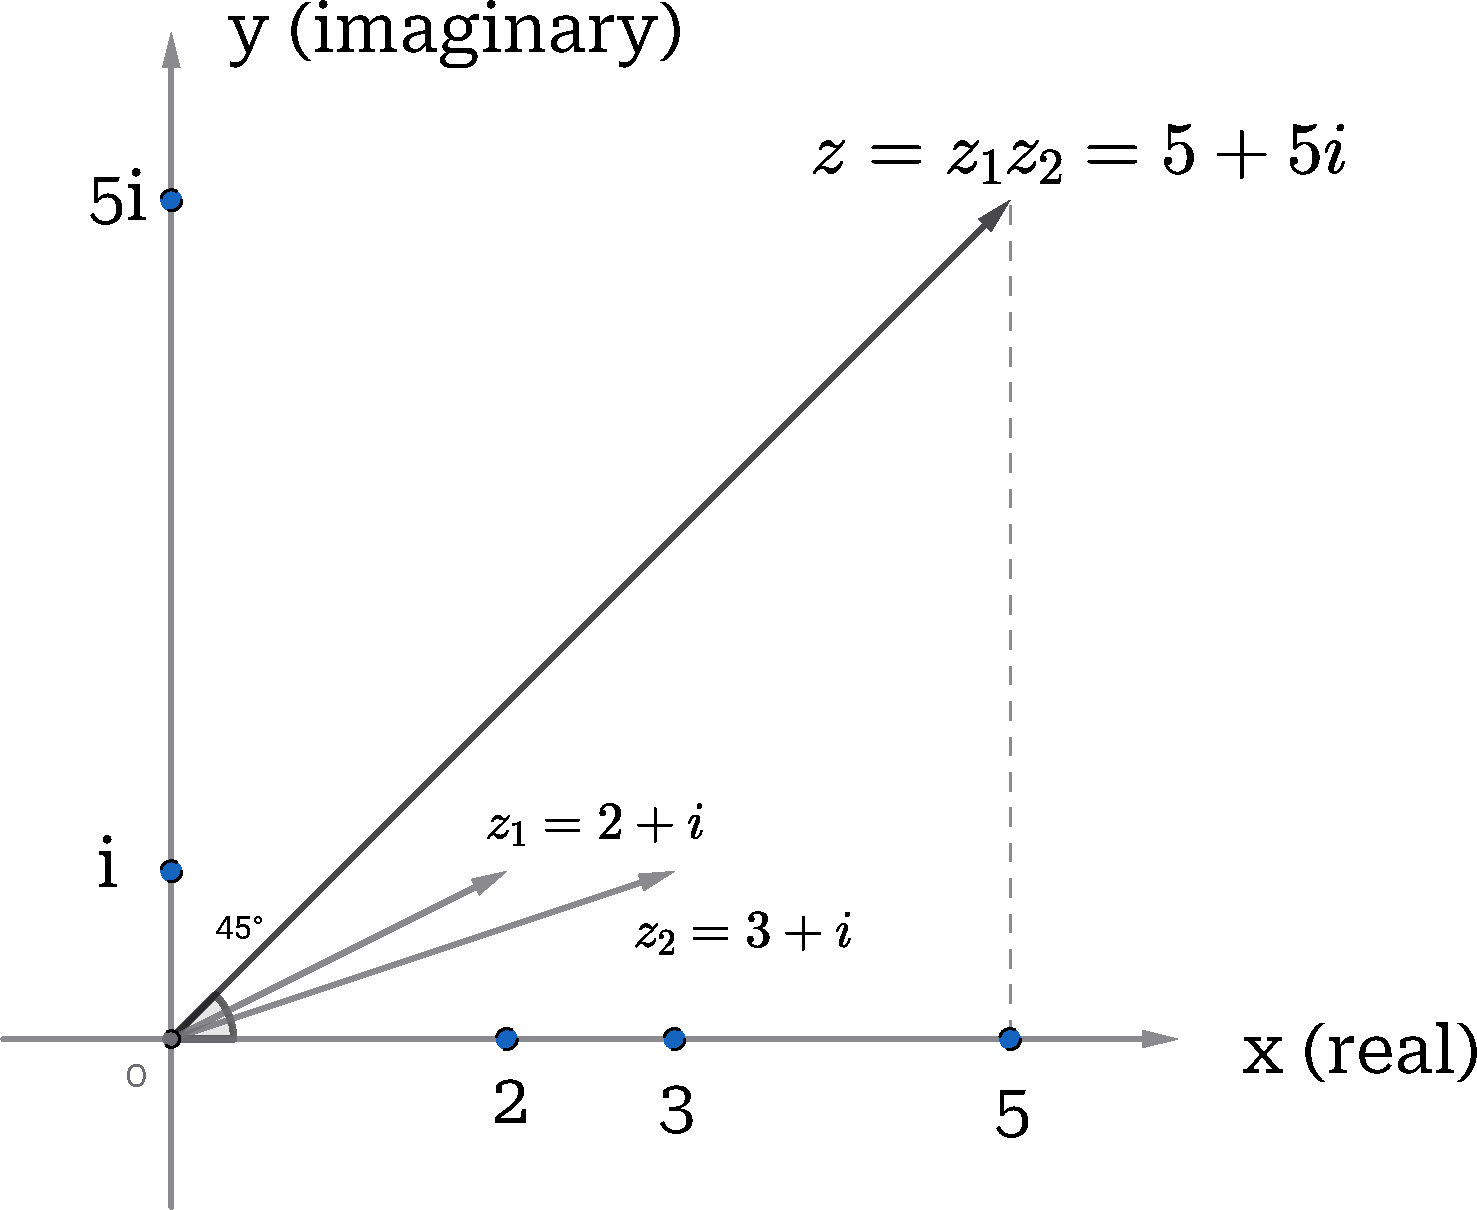
\includegraphics[scale=0.33]{img/machin1}
  \caption{$(2 + i)(3 + i) = 5 + 5i$}
 \label{fig:machin1}
\end{figure}

接下来证明麦钦公式:
\[
\frac{\pi}{4} = 4\tan^{-1} \frac{1}{5} - \tan^{-1} \frac{1}{239}
\]

\begin{proof}
令$z_1 = 5 + i, z_2 = 239 - i$。麦钦公式右侧幅角的4倍相当于$z_1^4$,我们构造复数乘积:

\begin{align*}
z &= z_1^4z_2 = (5+i)^4(239-i) \\
  &= (25 - 1 + 10i)^2(239 - i) && \text{完全平方公式} \\
  &= (24^2 - 100 + 480i)(239 - i) && \text{再次完全平方} \\
  &= 476 \times 239 + 480 + (480 \times 239 - 476)i && \text{展开} \\
  &= 114244 + 114244i
\end{align*}

$z$的幅角恰好是$\dfrac{\pi}{4}$
\end{proof}

这恐怕是麦钦公式最短最优美的证明。这个证明中还蕴含着一个复数的几何特性:如果复数$z = a + bi$的幅角是$\theta$,其中$b \ne 0$,则复数$a - bi$的幅角是$\tan^{-1}\dfrac{-b}{a} = -\theta$。记$\overline{z} = a - bi$为$z$的共轭复数。这样除以$a + bi$转动的角度相当于乘以$a - bi$所转动的角度。我们可以通过共轭复数方便地把除法转换成乘法。特别地:$z\overline{z} = (a + bi)(a - bi) = a^2 + b^2 = |z|^2$,因此:

\[
\frac{1}{z} = \frac{\overline{z}}{z\overline{z}} = \frac{1}{|z|^2}\overline{z}
\]

当模为1时,有$\dfrac{1}{z} = \overline{z}$,例如$z = \cos\theta + i\sin\theta$,我们立刻知道:

\[
\frac{1}{\cos\theta + i\sin\theta} = \cos\theta - i\sin\theta
\]

单位圆上的复数全都满足这个条件。\ref{qn:trigonometry-of-add}要求用复数运算推导三角函数的和角公式。

\subsection{代数基本定理}

一旦引入复数并赋予它几何意义,人们再回过头来看二次方程就发现原来无解的情况变得有解了。例如卡尔达诺在《大术》中的题目:两个数相加等于10,相乘等于40,即$(5 + x)(5 - x) = 40$,利用平方差公式展开整理得:$x^2 + 15 = 0$。它没有实数解,但是却有两个复数根:$x_{1,2} = \pm i\sqrt{15}$;多项式$x^2 + 15$用实数无法因式分解,但是却可以用复数分解为因式$(x + i\sqrt{15})(x - i\sqrt{15})$。而且让人惊喜的是,原来复杂的三种情况:(1) 有两个不同的实根,(2) 有两个相同的实根,(3) 无实数解,在复数中一下子变得简单一致了:任何二次方程有两个复数根,重根算作两个。数学家都是极简完美主义者,谁也无法抗拒这样优美的结论。那么三次方程呢?四次方程呢?以及更高次方程呢?笛卡尔发现了一个征服高次方程的有利武器。此外他还顺手引入了$x^n$这个记号。在笛卡尔之前,人们是用“平方”(square),“立方”(cube)这样的专门词汇来描述$xx$和$xxx$的,甚至有了专用名词quartic表示“四次方的”,quintic表示“五次方的”。但是显然$xxxx$,和$xxxxx$这样的符号太难用了。笛卡尔在1637年建立解析几何的时候,第一个引入了$x^3, x^4, x^5$这样的记号。我们再次看到好的符号是多么的重要!在历史的长河中,发展潮流是从“文辞”$\to$“简写”$\to$“符号”这样的方向演进的。很多人害怕充满了符号的公式,学生时期背公式是绝大多数成年人可怕的回忆。有些人因此一生讨厌数学,这实在是一个误解与遗憾。其实数学是最不需要记忆的一门课,因为我们可以靠着直觉、理性和审美,自己动手推出所有的结论。和很多人的感觉相反,符号比文字描述更简单、更容易理解、更精确,你可以比较一下文字描述“直角三角形一条直角边所构成的正方形的面积加上另外一条直角边所构成的正方形的面积等于斜边构成的正方形面积。”与代数符号$a^2 + b^2 = c^2$。

\begin{theorem}[笛卡尔]
多项式$p(x) = a_nx^n + \dotsb + a_1x + a_0$,其中$a_n \ne 0$。方程$p(x) = 0$有一个根$x = b$当且仅当多项式$p(x)$有一个因式$x - b$。
\end{theorem}

笛卡尔定理意味着如果$b$是根的话,多项式$p(x)$可以因式分解为$p(x) = (x - b)q(x)$,其中$q(x)$的次数比$p(x)$低。并且这是一个充分必要条件,所以反之亦真。我们可以方便地利用笛卡尔定理进行$x^3 - 1$的因式分解:显然$1$是方程$x^3 - 1 = 0$的根,所以$x - 1$是一个因式,然后用多项式长除法求出:

\[
\polylongdiv{x^3-1}{x-1}
\]

即使不会多项式长除法也没有关系,注意到等比数列求和公式$1 + x + x^2 + \dotsb + x^{n-1} = \dfrac{x^n - 1}{x - 1}$,就可以因式分解$(x^3 - 1) = (x - 1)(x^2 + x + 1)$了。

\begin{proof}
如果$x - b$是$p(x)$的一个因式,则$p(x) = (x - b)q(x)$。代入$x = b$有$p(b) = (b - b)q(b) = 0$,因此$b$是一个根。

反之,我们把带余数的除法推广到多项式$a(x) = b(x)q(x) + r(x)$,其中$q(x)$相当于商,$r(x)$相当于余数,它的次数小于$b(x)$。若$x = b$是$p(x)$的一个根,即$p(b) = 0$。用带余数的除法求$p(x)$除以$x - b$,有$p(x) = (x - b)q(x) + r(x)$,其中$r(x)$的次数比$x - b$低。它只能是常数项$c$。代入$x = b$有$0 = p(b) = (b - b)q(b) + c$。因此余数$c = 0$,说明$p(x)$能被$x - b$整除,即$x - b$是$p(x)$的因式。
\end{proof}

笛卡尔定理给出了解决$n$次方程$p(x) = 0$的方法:\underdot{如果能}找到一个解$a$,然后提取出因式$p(x) = (x - a)q(x)$,接下来只需要解降低次数的方程$q(x) = 0$。\underdot{如果能}不断找到解,重复这个步骤,就可以彻底解决高次方程。1746年,法国数学家达朗贝尔(d'Alembert)注意到如果复数$z = a + bi$是方程$p(z) = 0$的解,则共轭复数$\overline{z} = a - bi$也是一个解(\cref{qn:conjugated-root}要求证明这一结论)。这就意味着如果方程有一个复数根,可以一下子把次数降低2次。你也许注意到了我们在“如果能”三个字下面加了点,遗憾的是,在实数范围内并不总能找到解,例如$p(x) = x^2 + 15 = 0$。但是在复数范围内呢?十八世纪的数学家们强烈意识到答案应该是“一定能”!

\begin{theorem}[代数基本定理]
任何多项式方程$p(x) = 0$都有一个复数根。
\end{theorem}

这个定理有着诸多的版本,吸引着众多聪明的头脑去证明它。高斯一生先后四次用不同的方法证明代数基本定理。1799年,22岁的高斯在其博士论文中证明了任何实系数多项式方程总有一个复数根。接着又在1815年和1816年给出了另外两个证明。1849年,在庆祝取得博士学位50周年的纪念会上,高斯又发表了第四个证明,并把多项式系数推广到了复数。一旦证明了任何多项式方程总有一个复数根,利用笛卡尔定理就能推出$n$次多项式方程总有$n$个复数根(包括重根):先找到一个根$z = a$,然后抽取因式$q(z) = p(z)/(z - a)$得到$n-1$次方程,重复此步骤就得到$n$个根。代数基本定理还能用因式分解的方式阐述:任何多项式都可以分解为若干一次式或二次式的积。然后利用达朗贝尔的结论,这些二次因式能再次分解为$(z - a)(z - \overline{a})$,所以可以等价地说:任何多项式可以在复数内分解为若干一次式的积。在大学的数学专业课上,能看到各种各样的代数基本定理证明方法,有利用伽罗瓦理论证明的,有利用拓扑学证明的,有利用数学分析证明的。我们这里给出阿尔冈的几何证明,这是所有证明中最简单易懂的。在阿尔冈之前,达朗贝尔于1746年给出过代数基本定理的证明。但高斯在1799年指出其中有“严重缺陷”,未经证明就使用了如下结论:

\begin{lemma}[达朗贝尔引理]
若非常数多项式$p(z)$在复数$z_0$处$p(z_0) \ne 0$,则在$z_0$的附近存在某个$z_0'$使得模$|p(z_0')| < |p(z_0)|$。
\end{lemma}

阿尔冈用复数的几何意义成功地证明了它,从而修复了这个缺陷。“非常数多项式”排除了$p(z) = 2$这样的多项式,它的值总是常数。“附近”实际上是\underdot{邻域}的概念,我们可以直观地想象以$z_0$为中心画一个小圆所覆盖的范围。$|p(z_0)|$表示多项式在$z_0$这一点所取复数值的模。

\begin{figure}[htbp]
  \centering
  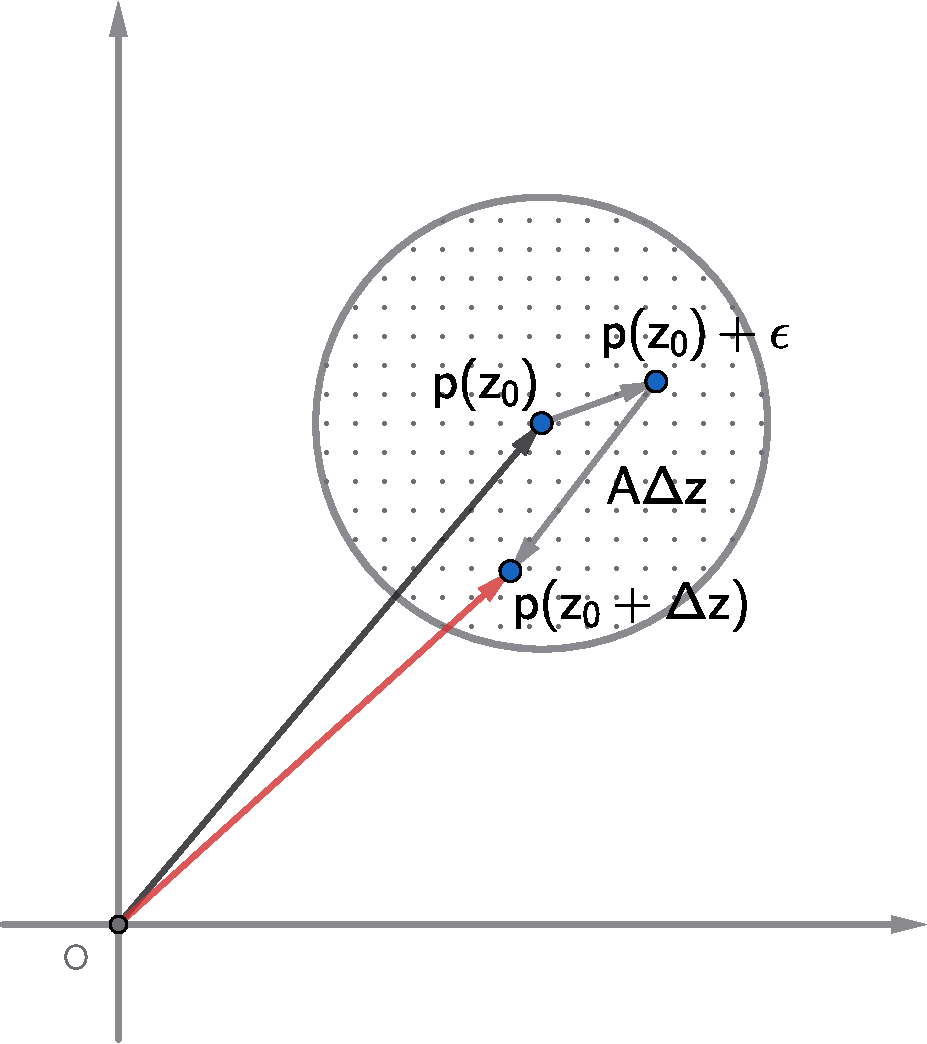
\includegraphics[scale=0.33]{img/dalambert-lemma}
  \caption{构造满足达朗贝尔引理的$p(z_0 + \Delta z)$}
 \label{fig:dalambert-lemma}
\end{figure}

\begin{proof}
还是一图胜千言。如\cref{fig:dalambert-lemma}所示,令多项式$p(z) = a_nz^n + \dotsb + a_1z + a_0$。它在复数$z_0$点的值$p(z_0)$是一个向量,长度为$|p(z_0)|$。阿尔冈要在$z_0$的附近找出一个$z_0' = z_0 + \Delta z$,此时多项式的值变成:

\begin{align*}
p(z_0 + \Delta z) &= a_n (z_0 + \Delta z)^n + \dotsb + a_1 (z_0 + \Delta z) + a_0  \\
 & \text{逐项二项式展开后整理} \\
 &= (a_n z_0^n + \dotsb + a_1 z_0 + a_0) + A_1 \Delta z + A_2 (\Delta z)^2 + \dotsb + A_n (\Delta z)^n \\
 &= p(z_0) + A \Delta z + \epsilon
\end{align*}

由于$p(z)$不是常数,所以$A_1, A_2, \dots A_n$不都是0。我们找到第一个不为0的$A_i$,令$A = A_i (\Delta z)^{i - 1}$,把剩余的部分放在一起叫做$\epsilon$。由于$\epsilon$含有更高次的$(\Delta z)^m$,当$|\Delta z|$变小时,会有$|\epsilon| < |A \Delta z|$。接下来阿尔冈选择一个$\Delta z$使得向量$A \Delta z$的方向与$p(z_0)$正好相反,起到了抵消作用。因此$|p(z_0 + \Delta z)| < |p(z_0)|$。
\end{proof}

但是阿尔冈对代数基本定理的证明也有一处缺陷:它依赖于极值定理(Extreme Value Theorem),即复数多项式的模值具有最小值。阿尔冈认为这是当然成立的(将其视为公理),这个定理后来由波尔查诺在1830年首先证明在实数上成立,1874年,魏尔斯特拉斯证明了它在复数上也成立:

\begin{theorem}[极值定理]
连续函数在有界闭集上存在最大值和最小值。
\end{theorem}

利用达朗贝尔引理和极值定理,我们就可以重建阿尔冈的证明了。

\begin{proof}
对任意复数多项式$p(z)$,考虑连续函数$|p(z)|$。当$|z|$很大时,$p(z) \approx a_n z^n$,最高次项主导了函数值。随着$|z|$的增大,连续函数值$|p(z)|$将会超过一个足够大的圆$|z| = R$。注意到$|z| \leq R$是一个有界闭集,根据极值定理,$|p(z)|$在其中存在最小值。由复数模的定义(向量的长度),这个最小值$\geq 0$。但如果最小值$> 0$,就会和达朗贝尔引理矛盾:总可以在附近找到一个模更小的值,从而比最小值更小。因此最小值只能是0,即存在某个$z_0$使得$|p(z_0)| = 0$,所以$p(z_0) = 0$。
\end{proof}

这样就证明了代数基本定理,任何多项式方程都有一个复数根。读到这里,有些朋友恐怕要摩拳擦掌、跃跃欲试准备自己动手解4次方程、5次方程甚至更高次的方程了。且慢!4次方程的确有求根公式公式,但\underdot{一般}的5次以上方程不存在求根公式。它们的解的确存在,但是不能用系数的加减乘除和开方运算表达。从卡尔达诺和费拉里之后,数学家们经过了300年才最终揭开了这个秘密。意大利数学家鲁菲尼和挪威数学家阿贝尔先后证明了这一结论\footnote{鲁菲尼1799年的证明存在瑕疵,阿贝尔于1823年首次严格证明了这一结论。这一定理今天叫做阿贝尔——鲁菲尼定理。}。注意这里说的“一般”是指$ax^5 + bx^4 + cx^3 + dx^2 + ex + f = 0$这种形式,特殊的5次方程是有公式解的,例如$x^5 - 1 = 0$,我们甚至可以通过解这个方程找出正五边形的尺规作图方法(见第\ref{sec:pentagon-equation}节)。什么样的方程根式可解的问题是由法国数学家伽罗瓦彻底解决的。这一理论叫做伽罗瓦理论。

\begin{figure}[htbp]
  \centering
  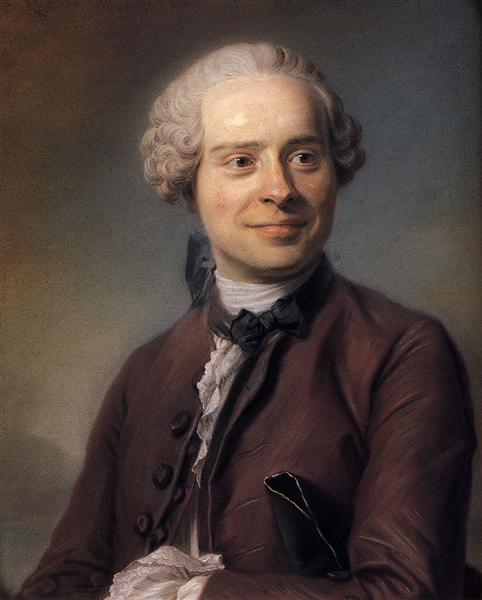
\includegraphics[scale=0.33]{img/d-alembert}
  \caption{法国洛可可风格肖像莫里斯・康坦・德・拉图尔于1753年创作的《达朗贝尔》,藏于卢浮宫}
 \label{fig:dalembert}
\end{figure}

\begin{mdframed}
让・勒朗・达朗贝尔(1717~1783)是法国著名的数学家、物理学家、天文学家。他是一位被遗弃的私生子。这一身世影响了他的一生。达朗贝尔的生父是一位炮兵军官,生母是一位巴黎著名沙龙\footnotemark 的女主人。达朗贝尔是这位交际花诸多风流韵事之一的结果,但他一出生就被生母遗弃在巴黎圣·乐朗教堂的台阶上。他因此得名让·乐朗(以捡到的地方命名)。一位好心的玻璃匠夫妇收养了可怜的孩子,达朗贝尔终身视他的养母为自己的亲生母亲。

达朗贝尔的生父后来返回巴黎,暗中资助他接受教育。但1726年孩子9岁的时候,他的生父死了。他被送入一所詹森教派的学校。在入学时他的姓氏是达朗伯格(Daremberg),不久后他改名为让·达朗贝尔(Jean dA'lembert)。詹森派学校主要培养神学人才以宣扬教义,但达朗贝尔只对数学感兴趣而不喜欢神学。他接触了笛卡尔的学术思想,虽大开眼界但并不以为然。1735年毕业后,达朗贝尔决心学习法律。他于1738年拿到了律师证书,但接着又改学医学。达朗贝尔不久再次改变了想法,他觉得医学还不如神学,自己的真爱还是数学。达朗贝尔基本上是自学数学,并且从未间断,即使是在准备律师考试期间。

长期的自学既造就了出众的独立思考能力和创造力,也限制了达朗贝尔。他一生不断提出新思想,开拓新方向,却不擅长深入推进、清晰阐述,很快被别人超越。这些新想法的支持者最终变成了达朗贝尔的竞争者。这使得他与其他学者争吵不断,抱怨别人抄袭窃取他的成果。尽管如此,达朗贝尔在数学、物理、天文学上做出了非常杰出的贡献。1739年,22岁的达朗贝尔在巴黎科学院暂露头角,1741年成为科学院正式成员。1743年,他发表了著作《动力学》,其中包括牛顿运动定律新的表述,并提出了今天以他命名的“达朗贝尔原理”。这一原理可以把动力学问题转化为静力学问题处理,为分析力学的创立打下了基础。次年,他成功应用这一原理研究了流体静力学和动力学,并由此开拓了偏微分方程这一数学分支。这使他获得了1747年柏林科学院大奖。达朗贝尔接着把偏微分方程应用到弦振动上,首次给出了波动方程。这一工作引起了欧拉的注意和支持。欧拉很快在偏微分方程上展开研究,超越并取得了硕果。两人的关系逐渐恶化,达朗贝尔忿忿不平,认为欧拉窃取了他的想法。但达朗贝尔的原文混乱不清,难以理解,欧拉干脆另起炉灶,从头推导出了更丰富的结果。达朗贝尔严格对待极限概念,是当时极少数把微分看成是函数极限的数学家,并区分了收敛与发散级数。他还提出了一种判别级数绝对收敛的方法——达朗贝尔判别法,即今天的比值判别法。另外,达朗贝尔在复数的性质、概率论等方面也都有所研究,很早就证明了代数基本定理。1764年,普鲁士大帝腓特烈二世想任命达朗贝尔为柏林科学院院长,但他拒绝了。俄罗斯女皇叶卡捷琳娜二世邀请达朗贝尔教授皇子保罗大公(Grand duke Paul),也被他拒绝了。

达朗贝尔生活的时代正值启蒙运动风起云涌。狄德罗、伏尔泰、卢梭的思想冲击着旧有的神权观念。达朗贝尔也投身到这场轰轰烈烈的变革中。受狄德罗邀请,达朗贝尔参与编写了法国《百科全书》。尽管合同上他只负责数学与天文学,但达朗贝尔热情地编写了广泛的内容,包括哲学、文学、音乐。达朗贝尔的后半生基本终止了数学研究,他把主要精力用来编写百科全书,从事社会活动。1772年,他当选了法兰西科学院终身秘书。但他对自己精力衰退,无法从事数学研究充满了遗憾。1777年,他写信给拉格朗日说\cite{MacTour-dAlembert}:“最遗憾的是,我无力研究我的真爱——数学了。我在文学上的工作——尽管在科学院备受赞扬——只能用来打发无聊的时间。”

特殊的身世冥冥之中影响着他。达朗贝尔终身未婚,他结识了巴黎著名沙龙的女主人勒皮纳斯(Julie de Lespinasse,1732~1776),并坠入爱河。达朗贝尔与养父母感情一直很好,直到1765年他47岁时才因病离开养父母,住到了勒皮纳斯家里。勒皮纳斯小姐于1776年去世后,达朗贝尔发现她还热烈地爱着其他男人。他伤心地搬到了卢浮宫的科学院公寓里\cite{Ronald-2024}。1783,达朗贝尔卒于巴黎。尽管达朗贝尔毕业于教会学校,尽管他在书中公开相信上帝的存在,但在狄德罗的影响下他转向了唯物论的观点。由于生前反对宗教,巴黎市政府拒绝为他举行葬礼。这位科学巨匠孤独地离开了人世。
\end{mdframed}
\footnotetext{法语Salon的音译,原指会客厅。从17世纪起,巴黎的名人(多半是名媛贵妇)常把客厅变成社交场所,组织谈论文化时事。沙龙渐成文艺集会的专称,风靡欧美各国文化界,十九世纪是它的鼎盛时期。}

复数的几何意义给出了直观解释,赋予了复数合法地位。但是另一些数学家坚持认为数作为数学抽象的典范,其形式本身就有意义。还记得范·德·瓦尔登用数偶$(a, b)$来形式化负数么(见第\ref{sec:z-as-pair}节)?数学家哈密尔顿(William Hamilton,1805~1865年)同样用数偶形式化了复数。1831年,哈密尔顿定义复数为一对值$(a, b)$,其运算规则如下:

\begin{itemize}
\item 复数加法:$(a, b) + (c, d) = (a + c, b + d)$
\item 复数乘法:$(a, b) (c, d) = (ac - bd, bc + ad)$
\end{itemize}

这个定义中,完全看不到声名狼藉的$\sqrt{-1}$。普通的实数表示为$(a, 0)$的形式,例如$-1$表示为$(-1, 0)$。虚数$i$表示为$(0, 1)$,我们可以验证$i^2 = -1$:

\[(0, 1)(0, 1) = (0 \times 1 - 1 \times 1, 1 \times 0 + 0 \times 1) = (-1, 0)\]

\cref{qn:pair-arithmetic-rules}要求验证五大定律(加法、乘法交换律、结合律、分配律)对复数都成立。这一定义明确强调了复数是由一对值复合而成的,复数的符号是$\mathbb{C}$,是Complex numbers的首字母。复数$z$的实部记做$Re(z)$,是Real的前两个字母;虚部记做$Im(z)$,是Imaginary的前两个字母。

%% 哈密尔顿简介

\section{$e$的诞生}

%% 英文版以莎士比亚《威尼斯商人》中安东尼奥向夏洛克借钱为例。
尽管阿尔冈图把复数、几何、三角函数联系在了一起,但这还不足以展示复数有多么神奇。真正让复数登堂入室、大放异彩的是另一个传奇常数$e$。但是$e$不像$\pi$那样在古代就被各个文明发现,它隐藏在大自然的背后,支配着生命的繁衍、财富的积累、时间的流逝……直到微积分的风帆乘风破浪开始远航的时候,人们才终于认识了e的庐山真面目。1683年,瑞士数学家雅各布·伯努利(Jacob Bernoulli, 1655~1705)思考了财务上的“复利”问题。所谓复利,又叫做“利滚利”,常见于可怕的高利贷中。比如杨白劳向黄世仁借了100元钱,每月利息为5\%(俗称五分利,是古代典型的高利贷)。一个月后杨白劳本息合计要还$100 \times (1 + 5\%) = 105$元钱。如果杨白劳没有还上,到了两个月的时候,此时要还的钱是$100 \times (1 + 5\%) \times (1 + 5\%) = 100 \times (1 + 5\%)^2 = 110.25$元。注意到第一个月后的利息被加到了本金中,用来计算第二个月应还的钱。因此叫做“利上加利”或“利滚利”。复利是指数增加的,也就是俗称的“指数爆炸”。如果杨白劳从年初一直到借到年底,那么要还的钱是$100 \times (1 + 5\%)^{12} = 179.59 \approx 180$元;两年的话就欠下$322.5$元的债务,已经是原来本金的三倍多了。雅各布·伯努利思考的问题是关于储蓄的,如果存入银行100元,年利是100\%,那么年底时本息合计就得到$200$元。如果每6个月时取出所有本息,然后再次存入银行。假设银行连续计息,6个月时的利息不到100\%,只有50\%。但到年底时共计息两次,所以本息合计$100 \times (1 + \frac{1}{2}\times 100\%)^2 = 225$元。这样比一次性到年底取钱能得到更多。假设每个季度取出所有本息再次存入,那么共计息4次,每次$25\%$,年底获得$100 \times (1 + \frac{1}{4} \times 100\%)^4 \approx 244.14$元。假如每个月都取出再存入银行,到年底获得$100 \times (1 + \frac{1}{12} \times 100\%)^{12} \approx 261.3$元。据此,把年底所得除以本金100元就可以推出\underdot{实际年化}利率\footnote{在银行业,年化利率(Annual Percentage Rate, APR)和\underdot{实际}年化利率(Internal Rate of Return, IRR)是不同的概念。前者是单利计算,后者是复利(利滚利)。}和存取次数$n$之间关系:

\be
(1 + \frac{1}{n})^n
\ee

雅各布·伯努利发现尽管增加存取次数(频率)会增加收入,但并非无限增加。增加的速度越来越缓慢,渐渐趋于一个定值,如\cref{tab:compound-interest}所示。他于是定义了一个常数,它的值是$n$趋向于无穷时的极限:

\begin{table}[ht]
  \caption{复利与存取次数的关系}
  \centering
  \begin{tabular}{|l|l|l|}
    \hline
    间隔 & 次数$n$ & 实际年化利率 \\
    \hline
    年 & 1 & 2 \\
    半年 & 2 & 2.25 \\
    季度 & 4 & 2.4414 \\
    月 & 12 & 2.6130 \\
    天 & 365 & 2.7146 \\
    小时 & 8760 & 2.7181 \\
    \hline
  \end{tabular}
  \label{tab:compound-interest}
\end{table}

\be
e = \lim_{n \to \infty} (1 + \frac{1}{n})^n
\ee

这就是高中数学课上定义的常数$e$。它是数学史上第一个\underdot{用极限定义}的常数。但是雅各布·伯努利既没有给这个常数起名字,也没有耐心地计算出它的值。他只是利用二项式定理估计了这个常数的范围\cite{MacTour-e}:

\begin{proposition}[雅各布·伯努利]
常数$e$的范围是:\[2 < e < 3\]
\end{proposition}

\begin{proof}
\begin{align*}
e &= \lim_{n \to \infty} (1 + \frac{1}{n})^n \\
  &= 1 + \binom{n}{1}\frac{1}{n} + \binom{n}{2}\frac{1}{n^2} + \dotsb && \text{二项式展开} \\
  &= 1 + \cancel{n}\frac{1}{\cancel{n}} + \frac{n(n-1)}{2!n^2} + \frac{n(n-1)(n-2)}{3!n^3} + \dotsb \\
  &> 1 + 1 = 2
\end{align*}

另一方面
\begin{align*}
e &= 2 + \frac{1}{2!}\frac{n-1}{n} + \frac{1}{3!}\frac{n-1}{n}\frac{n-2}{n} + \dotsb \\
  &\leq 2 + \frac{1}{2} + \frac{1}{2 \cdot 3} + \frac{1}{2 \cdot 3 \cdot 4} + \dotsb && \text{每个}\frac{n-k}{n} < 1 \\
  &< 2 + \frac{1}{2} + \frac{1}{2 \cdot 2} + \frac{1}{2 \cdot 2 \cdot 2} + \dotsb && \text{不等式缩放} \\
  &= 2 + (\frac{1}{2} + \frac{1}{2^2} + \frac{1}{2^3} + \dotsb) \\
  &= 2 + 1 = 3 && \text{等比数列和} \qedhere
\end{align*}
\end{proof}

读者朋友也许会问:(1) 以往只说数学家的姓就足够了,为什么这里既有名(雅各布)也有姓(伯努利)?(2) 我记得高中课堂上说$e$是自然对数的底,它和复利有什么关系?这两个问题其实是相关的。雅各布还有一个弟弟名叫约翰·伯努利(见\cref{fig:Bernoulli-brothers})。后者从1697年开始研究了各种各样的指数函数。在此之前,人们仅仅把对数看成纯粹的数,而不是函数,甚至印刷出版了长长的对数表方便计算。约翰·伯努利从函数的角度把对数和指数联系了起来。

\begin{align*}
  y = a^x && x = \log_a y
\end{align*}

这是一对函数与反函数。当$a = e$时,就变成了:

\begin{align*}
  y = e^x && x = \ln y
\end{align*}

\begin{figure}[htbp]
 \centering
 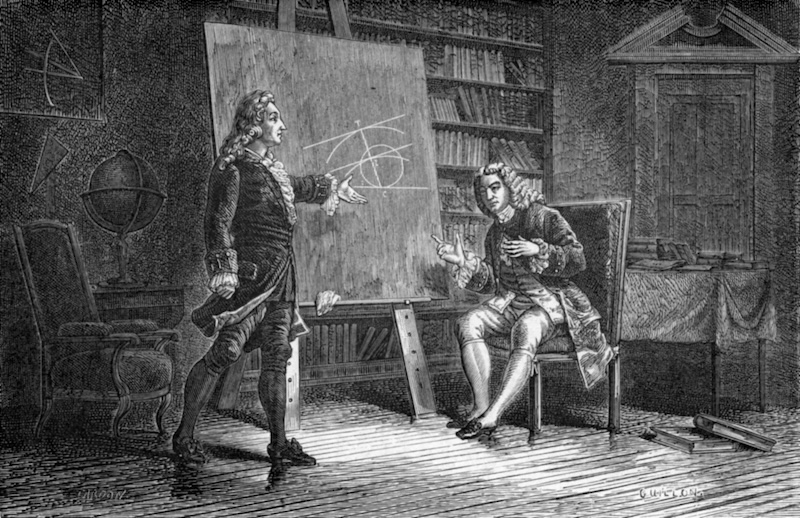
\includegraphics[scale=0.3]{img/Bernoulli-brothers}
 \caption{法国画家夏尔・约瑟夫・特拉韦尔创作的《伯努利兄弟讨论数学问题》}
 %% (Charles Joseph Traviers)
 \label{fig:Bernoulli-brothers}
\end{figure}

这样就把$e$的历史一下子向前推进到了1618年,苏格兰数学家约翰·纳皮尔发明了对数(见\cref{fig:napier}),并印出了第一张对数表。巧合的是最早的对数表的底不是10,而是自然对数$e$。当然纳皮尔并没有意识到常数$e$的存在,他只是想解决复杂的乘法计算问题。当时的天文观测和航海经常涉及巨大数字的乘法计算。我们今天知道,在计算$Z = XY$时,如果令$X = a^x, Y = a^y$,那么$Z = a^{x + y}$。所以我们只要在对数表中查到$X$和$Y$分别对应的对数$x$和$y$,把它们相加得$z = x + y$,然后在表中反查到对数$z$对应的数$Z$就可以了。后来英国数学家亨利・布里格斯提醒纳皮尔,改成以10为底的对数会更加方便实用。但当时纳皮尔已经垂垂老矣,无力再次进行巨大的计算以做出这个更改。淡泊名利的布里格斯于是亲自动手制作了以10为底的对数表,并以纳皮尔的名义发表\cite{Amerson-2021}。

从计算效率上来说,对数是一个化时代的发明,是大航海时代的产物。大家一定见过印在纸上的世界地图。把地球的球面不失真地映射到矩形纸上是一个困难的问题,这个问题在数学上是无解的。我们常见的世界地图叫做“墨卡托地图”,是用地理学家杰拉杜斯·墨卡托\footnote{Gerardus Mercator, 1512~1594,佛兰德斯(今比利时)地图绘制者和地理学家。}的名字命名的。墨卡托投影法想象把一张长方形的纸卷成圆筒,然后把透明的地球仪装入这个圆筒,使得赤道刚好和圆柱面相切(见\cref{fig:mercator})。此时在地球仪球心放一盏灯,在纸上就出现了地图的影子。把这个影子用笔描下来,再把纸展开就得到了墨卡托地图。墨卡托地图能很好地保持方向和形状,但是面积、距离越靠近两极越失真。

\begin{figure}[htbp]
 \centering
 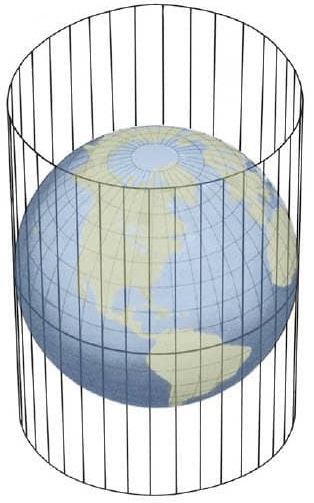
\includegraphics[scale=0.3]{img/mercator-map}
 \caption{墨卡托映射}
 \label{fig:mercator}
\end{figure}

无独有偶,和杰拉杜斯·墨卡托相同姓氏的德国数学家尼古劳斯·墨卡托于1688年的著作中把以$e$为底的对数命名为“自然对数”。尽管这项工作在雅各布·伯努利之后,但他并不知道$e$的存在和名字。我们要等欧拉来给这个传奇的常数命名。

\subsection{最美公式}

欧拉是约翰·伯努利的学生。当他沿着指数函数——对数函数的方向思考时,发现了一个惊人而又美丽的结果:$e^x$的导数是它本身。

\be
(e^x)' = e^x
\ee

\begin{proof}
根据导数的定义:

\be \label{eq:derive-of-e}
(e^x)' = \lim_{\Delta x \to 0} \frac{e^{x + \Delta x} - e^x}{\Delta x} = \lim_{\Delta x \to 0} \frac{e^xe^{\Delta x} - e^x}{\Delta x} = e^x\lim_{\Delta x \to 0} \frac{e^{\Delta x} - 1}{\Delta x}
\ee

欧拉把雅各布·伯努利对$e$的定义中的$n$取倒数,令$t = \frac{1}{n}$,得:

\be \label{eq:def2-of-e}
e = \lim_{n \to \infty} (1 + \frac{1}{n})^n = \lim_{t \to 0} (1 + t)^{\frac{1}{t}}
\ee

令$u = e^{\Delta x} - 1$,然后利用约翰·伯努利指出的对数函数与指数函数的反函数关系:$\Delta x = \ln (1 + u)$。代入上面的极限中:

\begin{align*}
\lim_{\Delta x \to 0} \frac{e^{\Delta x} - 1}{\Delta x} &= \lim_{u \to 0} \frac{u}{\ln (1 + u)} = \lim_{u \to 0} \frac{1}{\frac{1}{u}\ln (1 + u)} && \text{由} b \ln a = \ln a^b \\
  &= \lim_{u \to 0} \frac{1}{\ln (1 + u)^{\frac{1}{u}}} && \text{使用\cref{eq:def2-of-e}} \\
  &= \lim_{u \to 0} \frac{1}{\ln e} = 1 && \text{由} \ln e = 1
\end{align*}
将此结果带回\cref{eq:derive-of-e}就证明了$(e^x)' = e^x$
\end{proof}

这意味着二阶导数也是它本身,因为:$(e^x)'' = ((e^x)')' = (e^x)' = e^x$。不论对$e^x$求多少阶导数,得到的结果总是$e^x$。欧拉马上把这个结果代入麦克劳林公式(见\cref{eq:maclaurin})得到了著名的级数展开式:

\begin{align*}
e^x &= f(0) + \frac{f'(0)}{1!}x + \frac{f''(0)}{2!}x^2 + \dotsb + \frac{f^{(n)}(0)}{n!}x^n + \dotsb \\
  &= e^0 + \frac{e^0}{1!}x + \frac{e^{0}}{2!}x^2 + \dotsb + \frac{e^0}{n!}x^n + \dotsb && \text{各阶导数}f^{(n)}(x) = e^x \\
  &= 1 + \frac{x}{1!} + \frac{x^2}{2!} + \frac{x^3}{3!} + \dotsb
\end{align*}

有了展开式,欧拉就可以做出雅各布·伯努利不曾做到的东西了,求$e$的近似值。欧拉把$x = 1$代入展开式得到了著名的$e$的级数定义:

\be
e = 1 + \frac{1}{1!} + \frac{1}{2!} + \frac{1}{3!} + \dotsb
\ee

欧拉一口气算出了18位小数:$e = 2.718281828459045235$。这意味着他把级数的前20项计算出来,加到了一起。这一年是1731年,欧拉非常高兴地写信给好朋友哥德巴赫分享了这些成果。在信中,他给这个常数起了名字:“$e$”。很多人以为这是欧拉名字Euler的首字母,也有人说这是指数exponential的首字母,其实都不是。欧拉习惯使用元音字母a、e、i、o、u命名常量,碰巧a在之前已经被用过了,所以欧拉使用了第二个元音字母e。但这一巧合使得今天人们把$e$叫做“欧拉常数”以纪念他。

欧拉在信中明确指出了$e$是$n$趋近无穷时$(1 + \dfrac{1}{n})^n$的极限,并且等于1加上所有阶乘的倒数。他继续研究并于1748年发表了更加神奇优美的结果。欧拉把$e^x$级数展开中的奇数项和偶数项分开,并联想到著名的三角函数级数展开:

\begin{align*}
\sin x &= x - \frac{x^3}{3!} + \frac{x^5}{5!} - \frac{x^7}{7!} + \dotsb \\
\cos x &= 1 - \frac{x^2}{2!} + \frac{x^4}{4!} - \frac{x^6}{6!} + \dotsb
\end{align*}

欧拉发现了复数和$e$的关系,把自变量$ix$代入到级数展开中:

\begin{align*}
e^{ix} &= 1 + (ix) + \frac{(ix)^2}{2!} + \frac{(ix)^3}{3!} + \frac{(ix)^4}{4!} + \dotsb \\
  &= 1 + ix - \frac{x^2}{2!} - i\frac{x^3}{3!} + \frac{x^4}{4!} + \dotsb && i^2 = -1\\
  &= (1 - \frac{x^2}{2!} + \frac{x^4}{4!} - \frac{x^6}{6!} + \dotsb) + i(x - \frac{x^3}{3!} + \frac{x^5}{5!} - \frac{x^7}{7!} + \dotsb ) \\
  &= \cos x + i\sin x
\end{align*}

这就是高中数学课上的公式$e^{i\theta} = \cos \theta + i\sin \theta$。它右侧的几何意义极为明显:就是阿尔冈图上的模为1、幅角为$\theta$的复数。这样就赋予了$re^{i\theta}$几何意义,它是模为$r$、幅角为$\theta$的复数。进一步结合棣莫弗公式(见\cref{eq:de-Moivre})得:

\[
e^{in\theta} = \cos n\theta + i\sin n\theta = (\cos \theta + i\sin \theta)^n = (e^{i\theta})^n
\]

单位圆上幅角为$\theta$的向量的$n$次方相当于把向量旋转$n\theta$角。欧拉把特殊值$\theta = \pi$代入,得到了一个迷人的结果:

\be \label{eq:euler}
e^{i\pi} = \cos \pi + i\sin \pi = -1
\ee

人们把$e^{i\pi} + 1 = 0$叫做欧拉公式。许多人认为这是宇宙间最美的公式,它把两个著名的无理数$e, \pi$,虚数单位$i$,加法单位元0,乘法单位元1神奇地联系在了一起。

\begin{figure}[htbp]
  \centering
  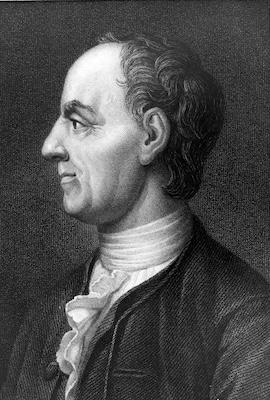
\includegraphics[scale=0.45]{img/Euler}
  \caption{莱昂哈德·欧拉}
 \label{fig:Euler}
\end{figure}

\begin{mdframed}
我们对欧拉的介绍主要来自大数学家安德烈·韦依的名著《数论:从汉谟拉比到勒让德的历史导引》。

莱昂哈德·欧拉生于1707年。那一年著名数学家雅各布·伯努利去世了,他的弟弟约翰·伯努利成为了瑞士巴塞尔大学的继任者。欧拉的父亲名叫保罗·欧拉,是巴塞尔附近的教区神父。他在巴塞尔大学学习神学的时候旁听过雅各布·伯努利的课程。他本来希望儿子也从事神职。小欧拉13岁进入巴塞尔大学神学院,主修哲学和法律,但很快就展现出在数学方面的天赋。每周六下午他都和约翰·伯努利学习数学。约翰·伯努利有两个孩子,尼古拉和丹尼尔。欧拉和他们成了好朋友,他也是约翰最得意的弟子。欧拉晚年时经常会想起他在星期六向伯努利学习数学时的情景。

三位君主在欧拉的一生中起到了决定性作用:彼得大帝、腓特烈大帝、叶卡捷琳娜大帝。彼得大帝年轻时去欧洲游历,回国后他决定兴建圣彼得堡,并仿照西方的样子建立科学院。1725年他去世后,科学院的计划得以继续。尼古拉和丹尼尔都被邀请加盟。遗憾的是,尼古拉于次年死于急性阑尾炎。于是,欧拉收到了圣彼得堡科学院的邀请。这一年他还不满20岁,刚刚凭借一篇关于造船的论文获奖,可他这辈子从未见过远洋轮船。他想离开家乡见见世面,于是欣然接受了。

欧拉从巴塞尔出发,顺莱茵河而下到达美因茨,然后步行前往吕贝克。在途中,他拜访了哲学家克里斯蒂安·沃尔夫。沃尔夫告诉欧拉,他被一位完全不懂哲学的国王赶出了柏林,流落至此。沃尔夫是莱布尼茨哲学的追随者,一心痴迷于莱布尼茨的单子论,而欧拉显然对此不以为然。离开吕贝克后,欧拉坐船到达圣彼得堡。

遵照彼得大帝的遗愿,科学院资金雄厚,拥有一流的图书馆。成员享有相当大的学术自由,主要目标就是开展一流的研究,发表高质量的论文,维护圣彼得堡科学院在国际学术上的崇高声誉。同时科学院向君主和政府提供顾问。尽管有些任务让学者们不快,不过毕竟国家出了巨资养活研究院,欧拉对此也完全理解。1727年欧拉到达圣彼得堡的时候,时局发生了变化。新沙皇中止了所有新任命。由于欧拉的获奖论文是关于造船的,他暂时被安排到俄罗斯海军部门。不久他获得了科学院的职位,头衔是“副教授”。1733年,丹尼尔·伯努利返回了瑞士巴塞尔,欧拉成了他的继任者,薪资大为改善。他开始安家置业,和一位瑞士侨民画家格赛尔的女儿结婚。次年大儿子约翰·阿尔伯特·欧拉出生了,他后来成了父亲的学术合作者、科学院的核心成员。欧拉和妻子一共生了13个孩子,但只有三个男孩活了下来。在俄国的14年中,他在分析学、数论和力学方面作了大量出色的工作。

欧拉在圣彼得堡安顿下来后,立即展现出超人的创造力,让所有人大吃一惊。另一方面,丹尼尔·伯努利的离去又让他倍感孤独。1735年,欧拉生了一场重病,以至右眼失明。后世我们看到的欧拉肖像,要么是侧面像(例如\cref{fig:Euler}),要么右眼部分被阴影遮住。毫无疑问,他已成为科学院最宝贵的成员,声誉如日中天。然而,欧洲政坛高层发生的两件大事,彻底打破了他平静的生活。1740年,沙皇皇后叶卡捷琳娜去世,随后摄政时期来临,政局动荡不安,科学院的存续似乎岌岌可危。恰逢此时,腓特烈二世从父亲(就是那位赶走哲学家沃尔夫的国王)那里继承了普鲁士王权\footnotemark。他雄心勃勃地着手建立柏林科学院,网罗全欧洲顶级的科学家。自然,欧拉在腓特烈大帝的名单上。欧拉收到了来自普鲁士国王的慷慨邀请,柏林优厚的待遇对比圣彼得堡混乱的时局,欧拉动心了。欧拉一家经过三周漫长的波罗的海航行,他自称是全家唯一没有晕船的人。终于1741年7月,他来到了腓特烈大帝面前。欧拉在这里愉快地渡过了25年。在柏林期间他的研究内容更加广泛,涉及行星运动、刚体运动、热力学、弹道学、人口学,这些工作和他的数学研究相互推动。欧拉这个时期在微分方程、曲面微分几何以及其它数学领域的研究都是开创性的。

搬到柏林丝毫没有减少欧拉在圣彼得堡科学院发表论文的数量。圣彼得堡不仅保留了他的科学院会员身份,还照常为他保留退休金。欧拉当然要让他的前同事觉得这笔钱花得值。在“惊人的25年”(欧拉曾孙语)中,欧拉寄给圣彼得堡超过100篇论文,在柏林发表了127篇论文,涵盖数学的方方面面,包括数学分析、造船、天文等等,他在巴黎科学院的论文获得大奖。随着时光流逝,腓特烈大帝和欧拉相互间的光环逐渐退去了。比起欧拉给科学院带来的巨大荣耀,腓特烈更钟情于法国文艺。他试图邀请达朗贝尔来柏林出任科学院院长,欧拉的自尊心受到了伤害。尽管达朗贝尔后来拒绝了国王的邀请,但欧拉在1763年起就考虑再次返回俄罗斯了。

此时的俄罗斯时局又发生了动荡。1762年,沙皇的德国妻子夺取政权,成为了叶卡捷琳娜二世。她决定重振圣彼得堡科学院,于是为欧拉打开了大门。对顶级人才的争抢持续了三年。终于,1766年,俄罗斯驻柏林大使受命让欧拉自己按照意愿撰写聘任合同(想怎么写就怎么写)。腓特烈大帝意识到问题的严重,想方设法阻挠。但太晚了,他不敢得罪这位女皇。欧拉被迎回圣彼得堡。途径波兰时,女王昔日的情人斯坦尼斯劳斯国王几乎按照君主的礼仪接待了欧拉。但不幸的是,欧拉左眼的视力也开始下降了。在1770年写给数学家拉格朗日的信中,他抱歉自己不能阅读,只能靠别人代为朗读,然后自己心算验证结果。1771年欧拉接受了眼科手术,起初效果很好,但很快感染了。欧拉不幸完全失明\cite{Weil-1983}。正如失聪没有阻止贝多芬的音乐创作一样,失明也同样没有阻止欧拉的数学探索\cite{HanXueTao2009}。在书记员的帮助下,欧拉在多个领域的研究其实变得更加高产了。在1775年,他平均每周就完成一篇数学论文。欧拉一生中有一半著作都是在双目完全失明后口述完成的。

欧拉渊博的知识,无穷无尽的创作精力和空前丰富的著作,都是令人惊叹不已的。他从19岁开始发表论文,直到76岁,半个多世纪写下了浩如烟海的书籍和论文。几乎每一个数学领域都可以看到欧拉的名字。欧拉是科学史上最多产的一位数学家,一生发表论文共计856篇,专著31部。这还不包括1771年圣彼得堡火灾中失去的一部分。这一记录直到20世纪才由匈牙利数学家保罗·埃尔德什打破,见第\ref{sec:Erdos}节。欧拉的多产并不是偶然的,他有着惊人的记忆力,还可以进行复杂的心算。法国物理学家阿拉戈说“欧拉计算时就像人在呼吸、鹰在翱翔一样轻松”。欧拉可以在任何不良的环境中工作,他常常抱着孩子在膝上完成论文,也不顾孩子在旁边喧哗。

欧拉的著作中既有难度很高的专著,也有专为普通大众所写的读物。他还特意为青少年写过一本书——《给德国公主的信》。并为非数学专业的读者写了一本初等代数教程,这本书至今仍在印刷。欧拉特别重视表达的清晰易懂。我们今天很多熟知的数学符号,都是欧拉精心选用的,例如$\pi$(1736年),虚数单位$i$(1777年),$e$(1748年),三角函数$\sin$和$\cos$(1748年),$tg$(1753年),$\Delta x$(1755年),求和$\sum$(1755年),表示函数的$f(x)$(1734年)等\cite{HanXueTao2009}。

1783年9月18日,欧拉与朋友们吃饭。那天天王星刚发现不久,欧拉列出计算天王星轨道的要领。晚餐后,欧拉一边喝着茶,一边和小孙女玩耍,突然之间,烟斗从他手中掉了下来。他说了一声:“我的烟斗”,并弯腰去捡,结果再也没有站起来,他喃喃地说了一句:“我死了……”就这样“停止了计算和生命”(法国数学家孔多塞语)。
\end{mdframed}
\footnotetext{需要区分两种称号:腓特烈二世(大帝)、神圣罗马帝国腓特烈二世(大帝)。后者为十二世纪皇帝(1194~1250年),而前者是普鲁士国王(1740~1786年),腓特烈二世是其正式名号,而“腓特烈大帝”是后世对其历史地位的尊称。}

\subsection{我依故我}
尽管没能看到欧拉的成果,但雅各布·伯努利在生前预见了$e^x$的诞生。1638年笛卡尔发现了一种神奇的螺线,名叫“等角螺线”,也叫做“对数螺线”(见\cref{fig:decartes-equiangular-spiral})。

\begin{figure}[htbp]
 \centering
 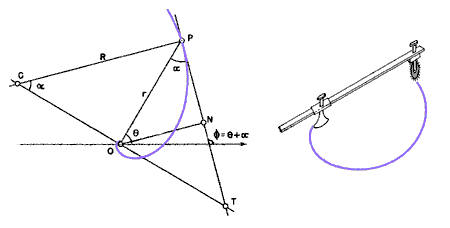
\includegraphics[scale=0.5]{img/descartesspiral}
 \caption{笛卡尔发现等角螺线}
 \label{fig:decartes-equiangular-spiral}
\end{figure}

顾名思义,笛卡尔发现螺线上任何一点的切线,与切点到原点连线的夹角是固定不变的,如\cref{fig:equiangular}所示\cite{Descartes-1638}。托里拆利\footnote{意大利数学家、物理学家。他首次通过实验测量了大气压。}对等角螺线进行了独立研究,他发现如果令$r$是原点$O$到螺线上一点$P$的距离,$\theta$是$OP$与横轴的夹角,如\cref{fig:decartes-equiangular-spiral}左侧。则随着$\theta$的增加$r$按照几何级数(即等比数列的方式)增加。这种定义是典型的极坐标定义,如果令曲线上一点为$(r, \theta)$,则托里拆利的定义相当于:

\begin{figure}[htbp]
 \centering
 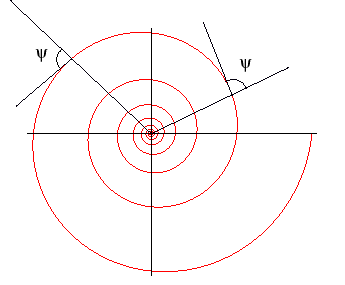
\includegraphics[scale=0.4]{img/equiangular}
 \caption{“等角”的含义}
 \label{fig:equiangular}
\end{figure}

\[
r = ka^\theta
\]

其中$k$和$a$是常数。这样$\theta$增加2倍,$r$就增加到$r^2$;$\theta$增加3倍,$r$就增加到$r^3$……\cref{qn:equiangular}要求证明托里拆利的定义和笛卡尔的定义是等价的。雅各布·伯努利对这种螺线进行了深入的研究,他发现了很多极有趣的性质。最令人震惊的是,不管怎么变化,缩放、求渐屈线、渐伸线、垂足线,结果总是不变——又得到了同一形状的螺线。1692年,他把这种迷人的螺线命名为“神奇螺线”(spiral mirabilis),并决定死后在墓碑上刻下这个螺线,如\cref{fig:bernoulli-tomb}所示\cite{MacTour-Equiangular}。他留下了著名的拉丁文墓志铭:Eadem mutata resurgo,中文译作“虽经沧海,我依故我”\cite{Maor-2010}。碑铭内容为:

\begin{figure}[htbp]
 \centering
 \subcaptionbox{雅各布·伯努利的墓碑\label{fig:bernoulli-tomb}}{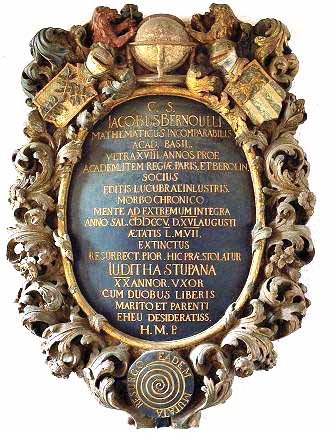
\includegraphics[scale=0.4]{img/bernoulli-tomb}}
 \subcaptionbox{墓碑下方的螺线\label{fig:bernoulli-epitaph}}{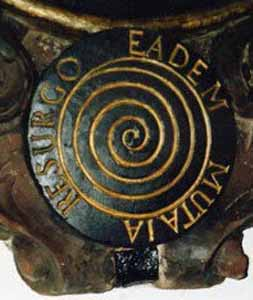
\includegraphics[scale=0.4]{img/bernoulli-epitaph}}
 \caption{雅各布·伯努利的墓志铭:Eadem mutata resurgo\cite{MacTour-Bernoulli-tomb}}
\end{figure}

\begin{mdframed}
\begin{verse}
雅各布·伯努利(1654-1705)\\
‌无与伦比的数学家‌\\
巴塞尔大学教授(18年)\\
巴黎科学院与柏林科学院院士\\
以学术著作闻名于世\\
虽罹患慢性疾病,却始终神志清明\\
于主历1705年8月16日安息,享年50岁又7个月\\
静候复活之日‌纪念者‌\\
朱迪丝·斯图潘努斯(20年结发之妻)\\
及其二子\\
为深切怀念的丈夫与父亲,立此碑铭
\end{verse}
\end{mdframed}

但遗憾的是,石匠错误地把等角螺线刻成了“阿基米德螺线”,如\cref{fig:bernoulli-epitaph}所示。这两个螺线有什么区别呢?阿基米德螺线每圈间的间距是相等的,而等角螺线的间距是等比数列(见\cref{fig:equiangular-spiral})。如果用极坐标表示,阿基米德螺线的方程是$r = a\theta$。匀速转动阿基米德螺线,则它与坐标轴的交点将匀速平移。那么为什么这种螺线又叫做“对数螺线”呢?从反函数的角度看:

\begin{figure}[htbp]
 \centering
  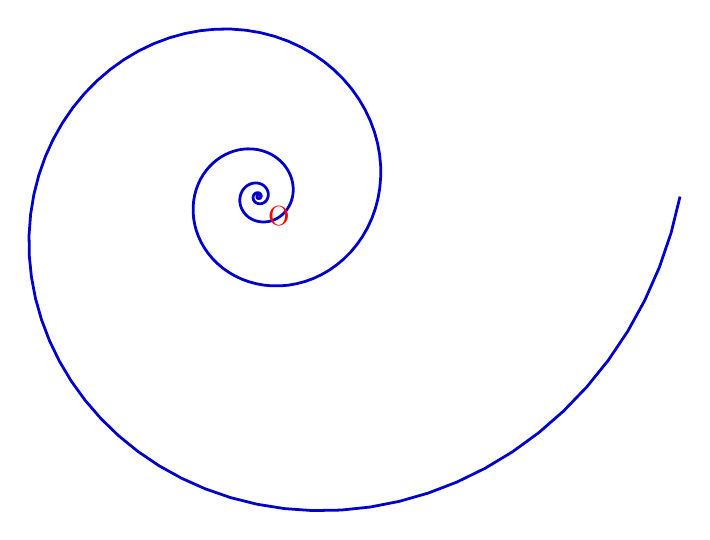
\begin{tikzpicture}[scale=0.1]
      % 定义对数螺线参数:r = a*e^(b*θ)
      \def\a{0.1}   % 控制螺线起点大小
      \def\b{0.2}   % 控制螺线旋紧程度(值越小越疏松)
      \def\turns{5} % 螺线旋转圈数

      % 绘制对数螺线
      \draw[
          line width=1pt,
          blue!80!black,
          domain=0:{2*pi*\turns},  % 角度范围(从0到指定圈数)
          samples=360,             % 采样点数(越多越平滑)
          variable=\t
      ] plot (
          {exp(\b*\t)*\a*cos(\t r)},  % x坐标(极坐标转直角坐标)
          {exp(\b*\t)*\a*sin(\t r)}   % y坐标(r表示弧度)
      );

      % 可选项:添加原点标记
      \fill[red] (0,0) circle (2pt) node[below right] {O};
  \end{tikzpicture}
  \caption{等角螺线也叫对数螺线}
  \label{fig:equiangular-spiral}
\end{figure}

\begin{align*}
r = ka^\theta && \theta = \log_{a} \frac{r}{k}
\end{align*}

螺线上一点的极角与极径成对数关系。因此法国数学家瓦里尼翁\footnote{Pierre Varignon,1654~1722年。曾系统整理和传播牛顿、莱布尼茨的微积分思想,并在力学中引入 “力矩”等重要概念。}把这种螺线叫做对数螺线。我们在高中学习过换底公式:$\log_a x = \dfrac{\ln x}{\ln a}$(\cref{qn:change-base}要求证明此公式),于是:

\begin{align*}
\theta &= \log_a \frac{r}{k} = \frac{\ln \frac{r}{k}}{\ln a} && \text{换底公式}\\
\ln \frac{r}{k} &= \theta(\ln a) && \text{两边同乘以}\ln a \\
\frac{r}{k} &= e^{\theta \ln a} = e^{b\theta} && \text{两边取}e\text{的指数,令}b = \ln a \\
r &= k e^{b\theta}
\end{align*}

这样就得到了以欧拉常数$e$为底的等角螺线极坐标方程。这个公式是雅各布·伯努利不曾想象到的,但它可以轻松揭示为何“我依故我”。

\begin{proposition}[雅各布·伯努利]
等角螺线缩放后形状不变。
\end{proposition}

\begin{proof}
利用等角螺线极坐标方程$r = ke^{b\theta}$,把极径缩放$a$倍得:

\begin{align*}
r' &= (ar)e^{b\theta} = e^{\ln a} k e^{b\theta} \\
   &= ke^{b\theta}e^{\ln a} = k e^{b\theta + \ln a} \\
   &= ke^{b(\theta + \theta_0)} && \text{令} \theta_0 = \frac{\ln a}{b}
\end{align*}

这相当于把极角旋转了$\theta_0$,而螺线旋转后的形状是不变的。
\end{proof}

\cref{qn:exp-from-fixed-point}要求利用“我依故我”的性质找出$e^x$的展开式。等角螺线还经由欧拉常数$e$和复数产生了联系。

\begin{proposition}
任何复数$z = a + bi, b \ne 0$构成的等比数列$z, z^2, z^3, \dotsc$都分布在等角螺线上。
\end{proposition}

\begin{proof}
用欧拉公式把$z$化成$z = c(\cos\theta_0 + i\sin\theta_0)$的形式,其中$c = \sqrt{a^2 + b^2}, \theta_0 = \tan^{-1} \dfrac{b}{a}$。因为$b \ne 0$,所以$\theta_0 \ne 0$。利用棣莫弗公式,等比数列的第$n$项为:

\[
z^n = c^n(\cos\theta_0 + i\sin\theta_0)^n = c^n(\cos n\theta + i\sin n\theta)
\]

我们接下来把$z^n$用极坐标表示,它的极角是$\theta = n\theta_0$,极径是:

\begin{align*}
r &= c^n = e^{\ln(c^n)} && \text{换底} \\
  &= e^{n\ln c} && \text{对数计算规则} \\
  &= e^{\frac{\theta}{\theta_0}\ln c} = ke^{b\theta} && \text{其中}k=1, b = \frac{\ln c}{\theta_0} \text{,满足等角螺线极坐标方程} \qedhere
\end{align*}
\end{proof}

等角螺线出现在自然界的各个角落,这并非偶然。棣莫弗利用待定系数法找出了斐波那契数列的通项公式,它在$n$很大时满足等角螺线方程(见附录\ref{app:fibonacci-formula})。而我们知道自然界很多生长现象满足斐波那契公式,例如鹦鹉螺的螺壳生长(见\cref{fig:nautilus}),西兰花、向日葵花絮的生长,因此呈现出等角螺线的形状。

\begin{figure}[htbp]
 \centering
 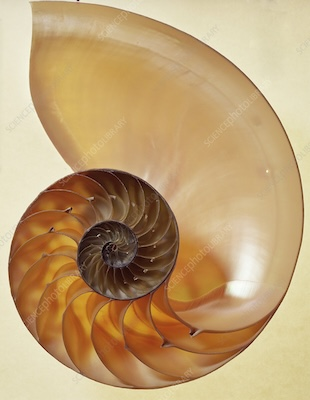
\includegraphics[scale=0.4]{img/nautilus}
 \caption{鹦鹉螺壳呈等角螺线}
 \label{fig:nautilus}
\end{figure}

复数和此前人们认识的数大相径庭。不管是自然数、有理数、无理数,它们都在数轴上有确定的位置。复数却跳出了数轴,来到了复平面。此前的数都是一元的,大小确定,在数轴上的位置确定。复数却是二元的,无论使用实部、虚部表示,模、幅角表示,都需要两个量来确定一个复数。两个复数通常没法比较大小,我们只能比较它们的模的大小。尽管这样奇特,复数彼此之间,复数与实数之间仍然可以计算,并且满足此前的运算定律,包括加法、乘法的交换律,结合率,乘法对加法的分配律。数轴上两个实数$a, b$间的距离是$|a - b|$,复平面上两个复数$z_1 = x_1 + y_1i, z_2 = x_2 + y_2i$间的距离是$|z_1 - z_2|$。这是因为:

\[
|z_1 - z_2| = |(x_1 - x_2) + (y_1 - y_2)i| = \sqrt{(x_1 - x_2)^2 + (y_1 - y_2)^2}
\]

这的确是对应的笛卡尔平面上两点$(x_1, y_1)$与$(x_2, y_2)$间的距离。实数的绝对值满足可乘性,即:$|ab| = |a||b|$;复数的模也满足可乘性$|z_1z_2| = |z_1||z_2|$,这是因为(也可用欧拉公式证明):

\begin{align*}
|z_1z_2|^2 &= |(x_1 + y_1i)(x_2 + y_2i)|^2 = |(x_1x_2 - y_1y_2) + (x_1y_2 + y_1x_2)i|^2 \\
  &= (x_1x_2 - y_1y_2)^2 + (x_1y_2 + y_1x_2)^2 = (x_1^2 + y_1^2)(x_2^2 + y_2^2) && (*) \\
  &= |z_1|^2|z_2|^2
\end{align*}

其中(*)是古希腊数学家丢番图最早在研究数论中的平方和时发现的\footnote{丢番图《算术》,卷三,问题19写道:65可以用两种方法分解为平方和$7^2 + 4^2$与$8^2 + 1^2$,这是因为65是13与5的乘积,而它们也都是平方和($13 = 3^2 + 2^2, 5 = 2^2 + 1^2$)。}。复数打开了一个新世界的大门。它威力无穷,不仅解决了以前的难题,也提出了人们意想不到的问题。

\section{正五边形}
\label{sec:pentagon-equation}

复数是解方程的利器。我们这里展示如何用复数解决正五边形尺规作图的问题。欧拉公式与棣莫弗公式结合赋予了方程$x^n = 1$以新的几何意义。若复数$z = re^{i\theta}$是方程的一个根,即:

\[
1 = z^n = (re^{i\theta})^n = r^ne^{in\theta} = r^n(\cos n\theta + i\sin n\theta)
\]

我们由此得出模$r = 1$,幅角$n\theta = 2k\pi$,其中$k$是整数(这是由于$\sin 2k\pi = 0, \cos 2k\pi = 1$),这样$z$的幅角$\theta = \dfrac{2k\pi}{n}$。于是根可以表示为:$z = 1e^{\frac{2k\pi}{n}i} = e^{\frac{2k\pi}{n}i}$。这在几何上表示复平面单位圆上的$n$个点,如\cref{fig:heptagon-z}所示。

\begin{figure}[htbp]
  \centering
  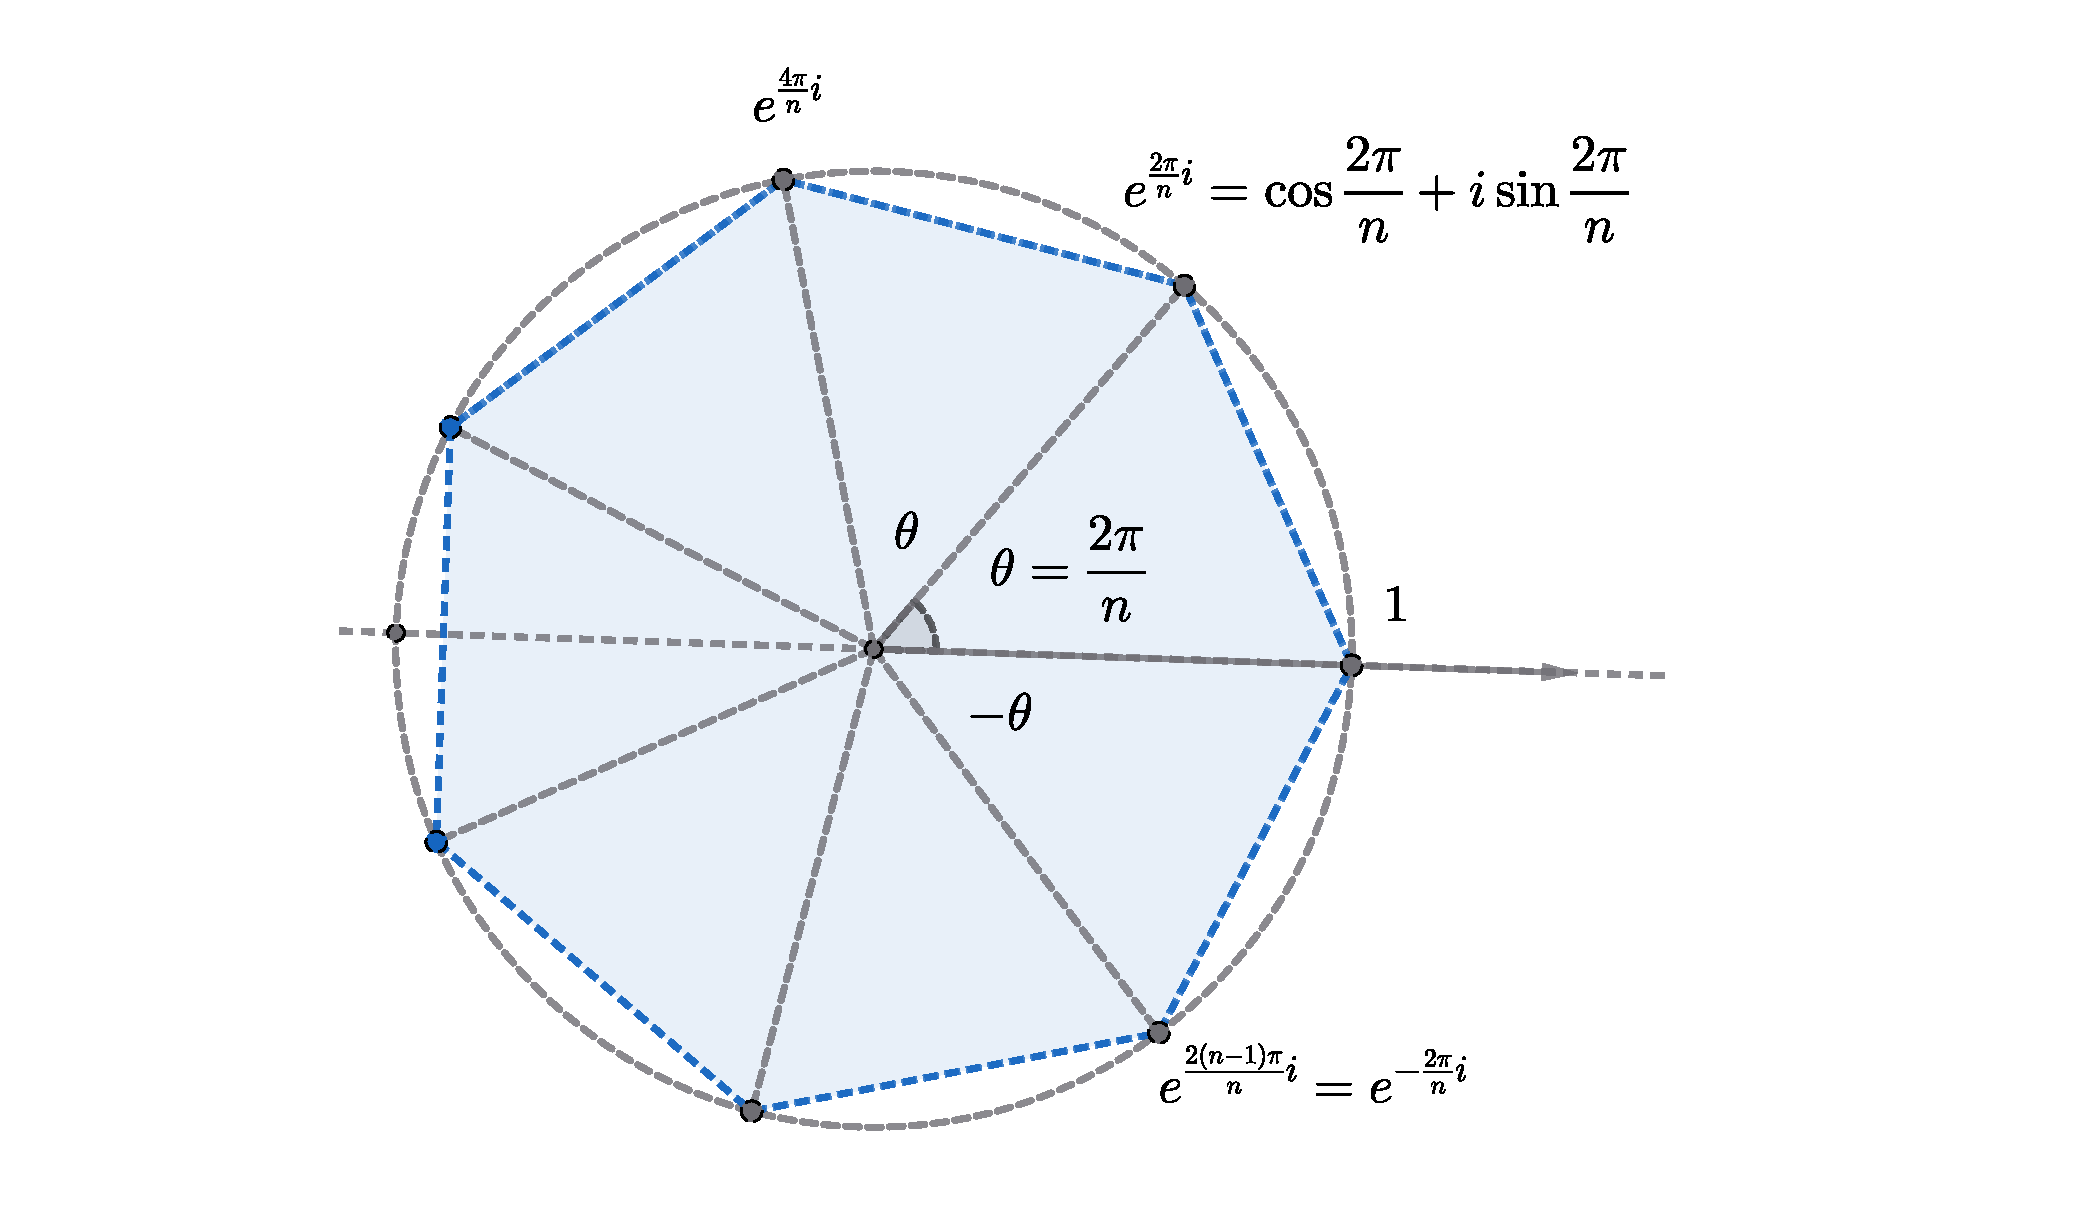
\includegraphics[scale=0.33]{img/heptagon-z}
  \caption{$x^n = 1$的解在复平面上是正$n$边形的$n$个顶点。}
 \label{fig:heptagon-z}
\end{figure}

圆是周期性的,$e^{\frac{2k\pi}{2}}$转动整数圈后与自己重合。$k = 0, 1, 2, \dotsc, n-1$时,$e^{\frac{2kp}{n}i}$是$n$个不同的根。它们的幅角依此是$0, \theta, 2\theta, \dotsc, (n-1)\theta$,把单位圆平均分成了$n$等份。因此方程$x^n = 1$叫做“分圆方程”(cyclotomic equation)。把复平面上这个$n$个根连接起来就构成了正$n$边形。

例如最简单的正多边形是正三角形$n = 3$。$x^3 = 1$有三个复根$1, e^{\frac{2\pi}{3}i}, e^{\frac{4\pi}{3}i} = e^{-\frac{2\pi}{3}i}$。其中:

\[
e^{\pm \frac{2\pi}{3}i} = \cos (\pm \frac{2\pi}{3}) + i \sin (\pm \frac{2\pi}{3}) = -\frac{1}{2} \pm \frac{\sqrt{3}}{2}i
\]

我们可以验证$x^3 - 1 = (x - 1)(x^2 + x + 1)$,二次方程$x^2 + x + 1$的两个根的确是$\dfrac{-1 \pm i\sqrt{3}}{2}$。我们也可以用二项式展开直接验证:

\[
(-\frac{1}{2} \pm \frac{\sqrt{3}}{2}i)^3 = -\frac{1}{8} \pm \frac{3\sqrt{3}}{8}i + \frac{9}{8} \mp \frac{3\sqrt{3}}{8}i = \frac{9-1}{8} = 1
\]

这三个根构成了单位圆内接正三角形,如\cref{fig:3rd-root-of-1}所示。

\begin{figure}[htbp]
\centering
\begin{tikzpicture}[scale=2.5]
 \draw[step=.5cm, gray, very thin] (-1.2,-1.2) grid (1.2,1.2);
 \draw[->] (-1.25,0) -- (1.25,0) coordinate (x axis)
   (0,-1.25) -- (0,1.25) coordinate (y axis);
 \draw (0,0) circle (1cm);
 \draw[->, very thick] (0, 0) edge node[below=2pt] {$e^0 = 1$} (1, 0)
   (0, 0) edge node[above] {$e^{\frac{2\pi}{3}i} = \dfrac{-1 + i\sqrt{3}}{2}$} (120:1cm)
   (0, 0) edge node[below] {$e^{\frac{4\pi}{3}i} = \dfrac{-1 - i\sqrt{3}}{2}$} (-120:1cm);
\end{tikzpicture}
\caption{$x^3 = 1$的三个复数根}
\label{fig:3rd-root-of-1}
\end{figure}

类似地,五次分圆方程$x^5 = 1$的五个根均匀分布在复平面的单位圆上,从而构成一个正五边形,如\cref{fig:pentagon-z}所示。只要求出图中的根$x$,则复平面上$x$到1的距离$|x-1|$就是正五边形的边长。五次方程$x^5 - 1 = 0$显然有一个根是$x = 1$。根据笛卡尔定理,$x-1$是多项式$x^5 - 1$的一个因式。利用多项式长除法(或逆向用等比数列求和)可以进行因式分解:

\[
x^5 - 1 = (x - 1)(x^4 + x^3 + x^2 + x + 1)
\]

接下来解四次方程$x^4 + x^3 + x^2 + x + 1 = 0$就可以找出\cref{fig:pentagon-z}中的剩余4个顶点。这个四次方程很有特点,只要除以$x^2$就变成一个对称的形式(0不是方程的解,因此$x \ne 0$):

\begin{figure}[htbp]
  \centering
  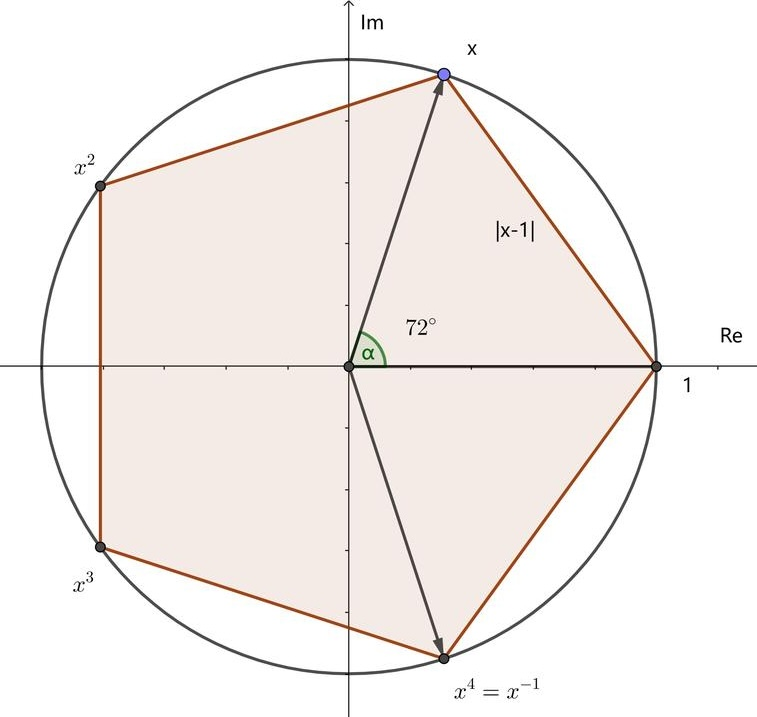
\includegraphics[scale=0.3]{img/pentagon-z}
  \caption{$x^5 = 1$的根在复平面上是正五边形的顶点。}
 \label{fig:pentagon-z}
\end{figure}

\[
x^2 + x + 1 + \frac{1}{x} + \frac{1}{x^2} = 0
\]

把$x + \dfrac{1}{x}$看成一个整体,并注意到:$(x + \dfrac{1}{x})^2 = x^2 + \dfrac{1}{x^2} + 2$。上面的方程可以化为:

\[
(x + \frac{1}{x})^2 + (x + \frac{1}{x}) - 1 = 0
\]

令$y = x + \dfrac{1}{x}$,上述方程就是$y^2 + y - 1 = 0$。解此二次方程得到$y_{1,2} = \dfrac{-1 \pm \sqrt{5}}{2}$。利用欧拉公式,若$x = e^{i\theta}$,则$\dfrac{1}{x} = x^{-1} = e^{-i\theta}$,所以$x, \dfrac{1}{x}$是共轭复数(见\cref{fig:pentagon-z}中的$x$与$x^4 = x^{-1}$)。若$x = a + bi$,则$\dfrac{1}{x} = a - bi$,所以$x + \dfrac{1}{x} = 2a$。同理\cref{fig:pentagon-z}中的$x^2, x^3$也是一对共轭复数,分别对应$e^{\frac{4\pi}{5}i}, e^{\frac{6\pi}{5}i} = e^{-\frac{4\pi}{5}i}$。这样我们就判断出:

\begin{align*}
x + \dfrac{1}{x} &= \dfrac{-1 + \sqrt{5}}{2} \\
x^2 + x^3 &= \dfrac{-1 - \sqrt{5}}{2}
\end{align*}

其中第一个方程本质上是二次方程$x^2 - \dfrac{\sqrt{5} - 1}{2}x + 1 = 0$,利用求根公式得:

\[x_{1, 2} = \dfrac{\frac{\sqrt{5} - 1}{2} \pm i\sqrt{\frac{5 + \sqrt{5}}{2}}}{2}
\]

它们是一对共轭复数,分别对应\cref{fig:pentagon-z}中的$x, x^4 = x^{-1}$。接下来计算\cref{fig:pentagon-z}中的模$|x - 1|$就知道正五边形的边长了。

\[
x - 1 = \frac{\frac{\sqrt{5} - 1}{2} + i\sqrt{\frac{5 + \sqrt{5}}{2}}}{2} - 1 = \frac{\sqrt{5} - 5}{4} + i\frac{\sqrt{\frac{5 + \sqrt{5}}{2}}}{2}
\]

因此:

\[
|x - 1| = \sqrt{(\frac{\sqrt{5} - 5}{4})^2 + (\frac{\sqrt{\frac{5 + \sqrt{5}}{2}}}{2})^2} = \frac{\sqrt{10 - 2\sqrt{5}}}{2}
\]

于是作正五边形的问题就转化为:任给长度为1的线段,如何做出长度为$s = \dfrac{\sqrt{10 - 2\sqrt{5}}}{2}$的线段。为了简化问题,我们先求线段$2s$。我们的思路是作一个直角三角形,使其斜边为$2s$。这个三角形的两个直角边不可能都是有理数,否则根据勾股定理,斜边不可能是$\sqrt{10 - 2\sqrt{5}}$这种根号下还有根号的形式。设两个直角边分别是$\sqrt{5} - a$和$b$,然后用勾股定理:

\[
(\sqrt{5} - a)^2 + b^2 = 5 + a^2 + b^2 - 2a\sqrt{5} = 10 - 2\sqrt{5}
\]

利用待定系数法,$2a = 2$,所以$a = 1$;代入$5 + a^2 + b^2 = 6 + b^2 = 10$,所以$b = 2$。这样直角边为$\sqrt{5} - 1, 2$的直角三角形的斜边是$2s$。将三角形缩小一半,直角边为$\dfrac{\sqrt{5} - 1}{2}, 1$的直角三角形的斜边就是$s$。另一方面,由于$5 = 4 + 1 = 2^2 + 1^2$,这样就可以用1,2为直角边,作出斜边长$\sqrt{5}$的直角三角形。缩小一半的直角三角形其斜边就是$\dfrac{\sqrt{5}}{2}$,然后再截去$\dfrac{1}{2}$就得到了$\dfrac{\sqrt{5} - 1}{2}$。\cref{fig:pentagon-cons}展示了尺规作正五边形的步骤。最后用求得的边长依次截单位圆五次就得到了正五边形。

\begin{figure}[htbp]
 \centering
 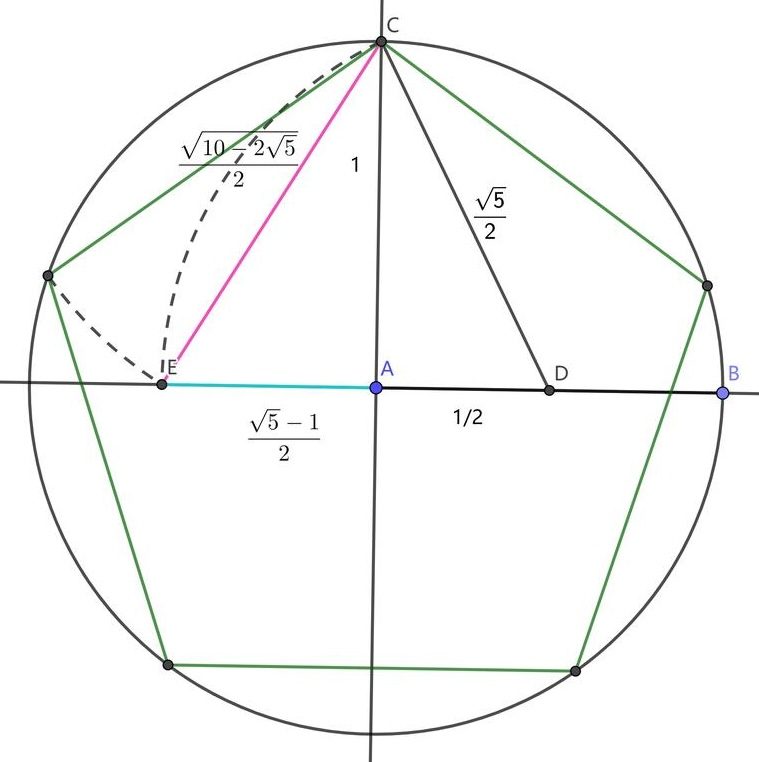
\includegraphics[scale=0.3]{img/pentagon-cons}
 \caption{作正五边形}
 \label{fig:pentagon-cons}
\end{figure}

\begin{Exercise}[label={ex:complex}]
\Question{给出解二次方程$x^2 - px = q$的几何解释。\label{qn:geometric-quadratic}}

\Question{根据代数基本定理,三次方程有三个复数根,卡尔达诺公式给出了方程$x^3 = 6x + 9$的一个根$x_1 = 3$,试求出方程的另外两个根。}

\Question{利用邦贝利的方法和卡尔达诺公式,可求出三次方程$x^3 = 15x + 4$的一个根$x_1 = 4$,试求出方程的另外两个根。}

\Question{计算规则$\sqrt{ab} = \sqrt{a}\sqrt{b}$在复数下是否成立?如果成立请证明之,如果不成立应怎样挽救?\label{qn:sqrt-of-product}}

\Question{证明任何复数代表的向量乘以$i$相当于向左转$90\degree$。\label{qn:mul-i}}

\Question{验证复数的共轭满足这样的运算规则:$\overline{a + b} = \overline{a} + \overline{b}$,$\overline{ab} = \overline{a} \cdot \overline{b}$, $\overline{z^n} = (\overline{z})^n$,并据此证明达朗贝尔的发现:若$z$是方程$p(z) = 0$的根,其共轭$\overline{z}$也是方程的根。\label{qn:conjugated-root}}

\Question{验证哈密尔顿的复数数偶表示满足五大运算定律。\label{qn:pair-arithmetic-rules}}

\Question{利用对数函数与指数函数的反函数关系证明换底公式$\log_a x = \dfrac{\log_b x}{\log_b a}$。\label{qn:change-base}}

\Question{*利用等角螺线的极坐标方程$r = ke^{b\theta}$证明笛卡尔指出的等角性质:螺线的切线和极径夹角$\Psi$不变(见\cref{fig:equiangular})提示:如\cref{fig:tagent-to-r}所示,极径$r$旋转过一个小角度$\Delta \theta$,极径增加了$\Delta r$。小圆弧$AC$长$r\Delta \theta$,它与割线$AB$,极径的增量近似组成一个直角三角形$ACB$。当$\Delta \theta \to 0$时,点$A, B$趋向重合,割线$AB$趋近于切线。\label{qn:equiangular}

  \begin{center}
    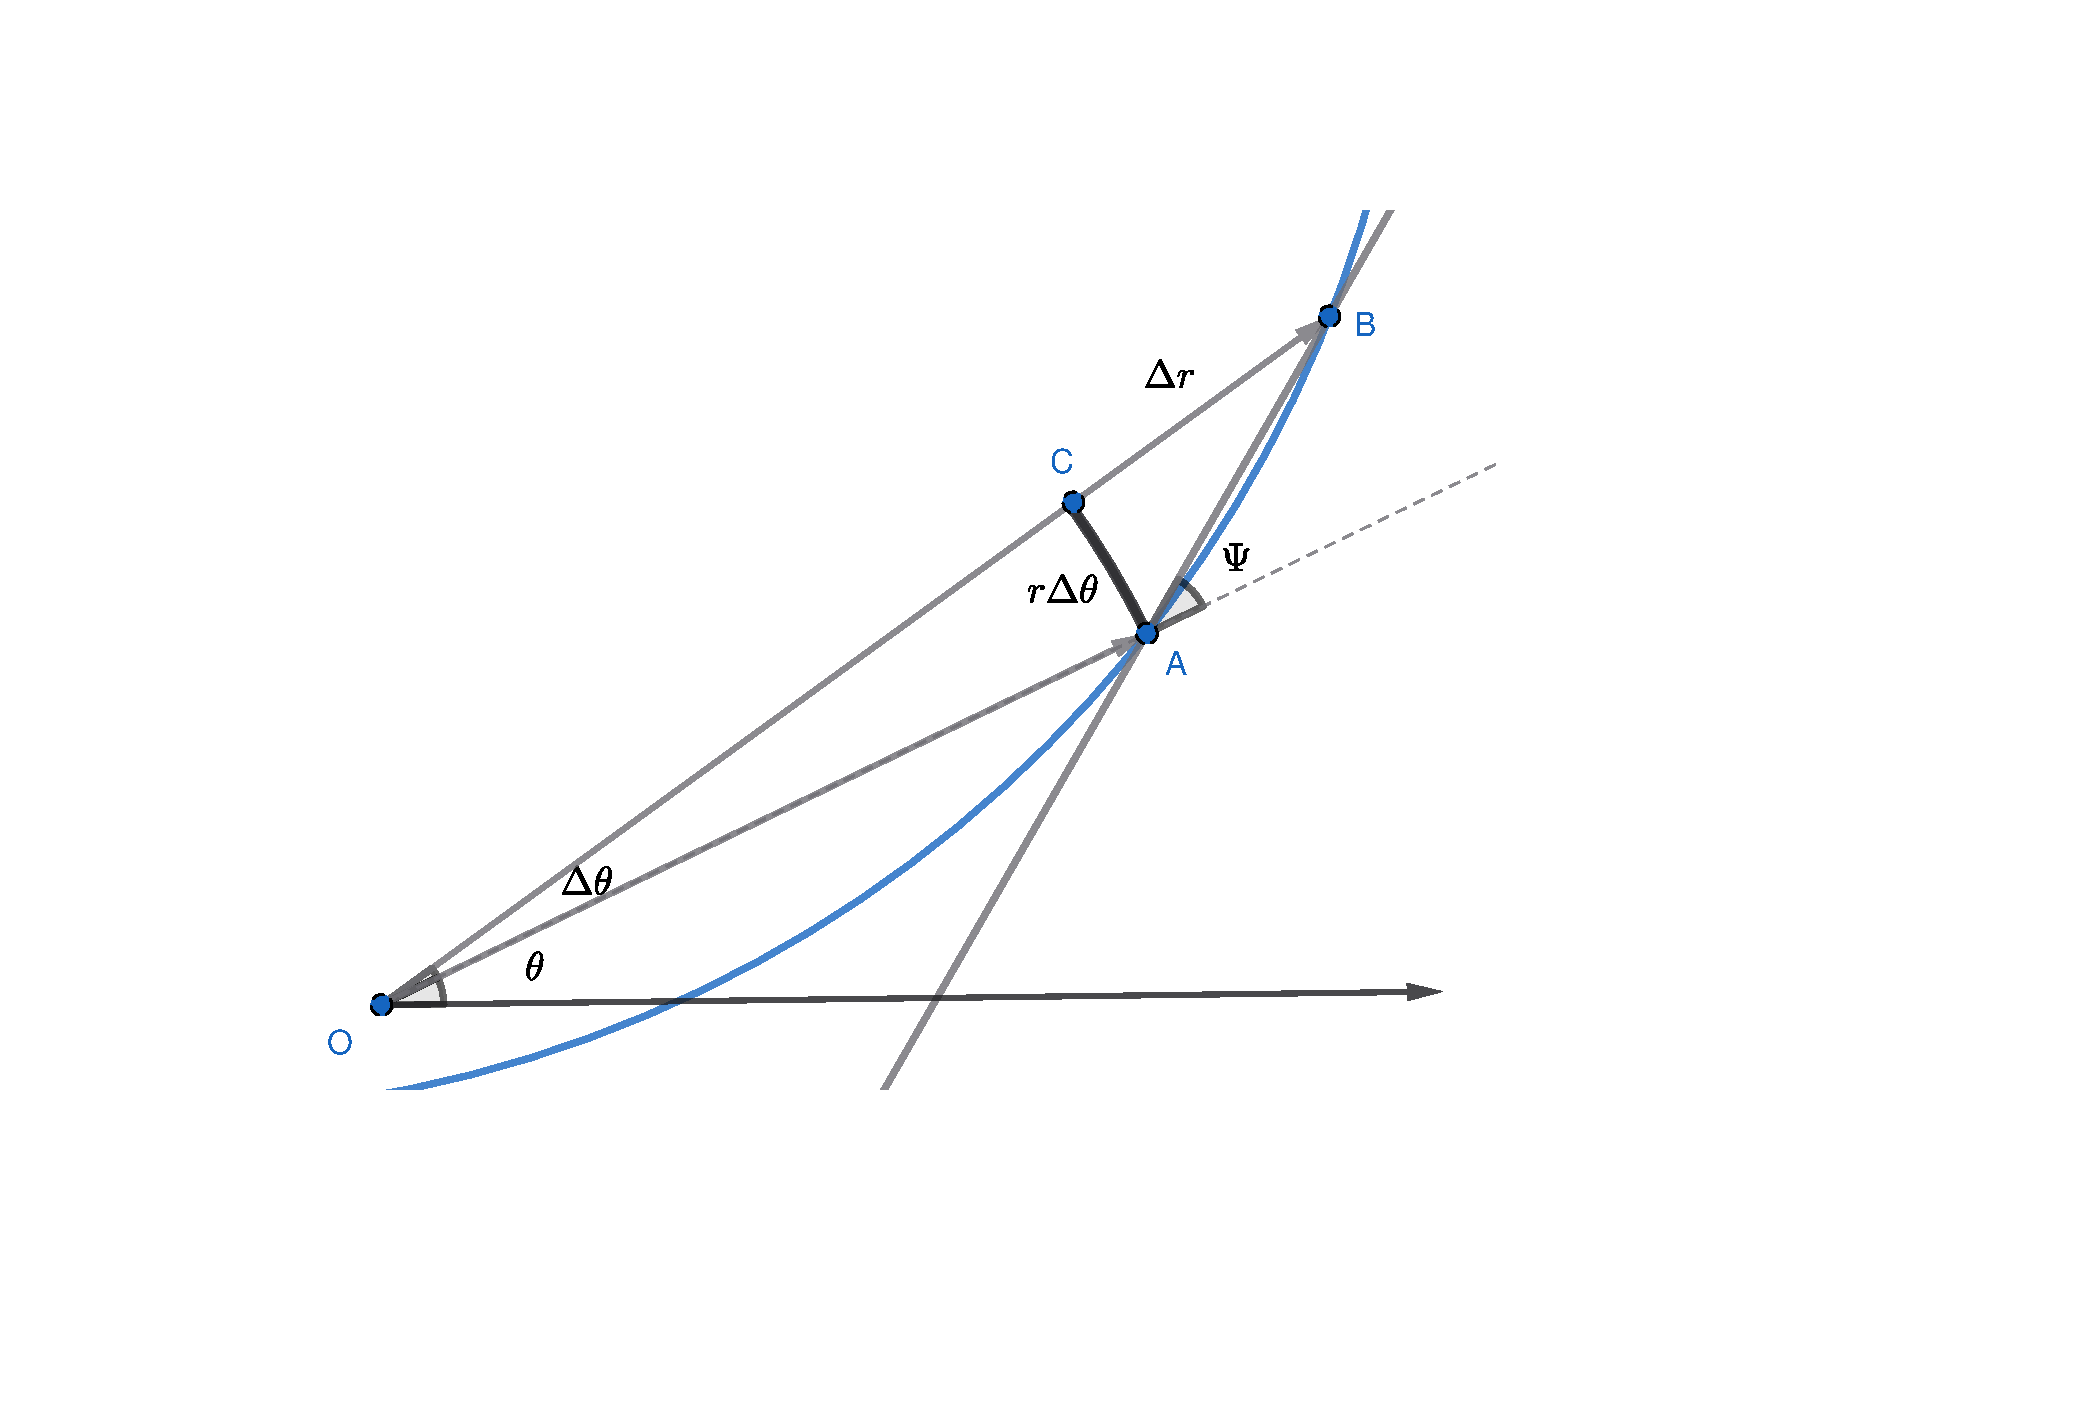
\includegraphics[scale=0.33]{img/tagent-to-r}
    \captionof{figure}{极径旋转小角度$\Delta \theta$}
    \label{fig:tagent-to-r}
  \end{center}
}

\Question{*雅各布·伯努利赞美的“虽经沧海,我依故我”也形象地描绘了求导不变$(e^x)' = e^x$的性质,现代数学家这样定义函数$f(x) = e^x$:(1) 导数不变$f'(x) = f(x)$,(2) 函数值$f(0) = 1$。试利用这个定义导出$e^x$的展开式。提示:待定系数法及$(x^n)' = nx^{n-1}$(见命题\ref{thm:derivation-of-power-of-x})。\label{qn:exp-from-fixed-point}}

\Question{*雅各布·伯努利距离发现$e^x$几乎只差一步。在计算复利时,如果年利率不是100\%,而是$x$,当$n \to \infty$时的实际年化收益率是什么?它的级数展开是什么?}

\Question{利用复数推导三角函数的和角公式:$\tan(\theta_1 + \theta_2), \sin(\theta_1 + \theta_2), \cos(\theta_1 + \theta_2)$,提示:复数乘法。\label{qn:trigonometry-of-add}}

\end{Exercise}

\begin{Answer}[ref={ex:complex}]
\Question{给出解二次方程$x^2 - px = q$的几何解释。

有两种情况:$q \geq 0$和$q < 0$
}

\Question{根据代数基本定理,三次方程有三个复数根,卡尔达诺公式给出了方程$x^3 = 6x + 9$的一个根$x_1 = 3$,试求出方程的另外两个根。

长除法或待定系数法
}

\Question{利用邦贝利的方法和卡尔达诺公式,可求出三次方程$x^3 = 15x + 4$的一个根$x_1 = 4$,试求出方程的另外两个根。}

\Question{计算规则$\sqrt{ab} = \sqrt{a}\sqrt{b}$在复数下是否成立?如果成立请证明之,如果不成立应怎样挽救?}

\Question{证明任何复数代表的向量乘以$i$相当于向左转$90\degree$。

\[(a + bi)i = ai - b
\]
}

\Question{验证复数的共轭满足这样的运算规则:$\overline{a + b} = \overline{a} + \overline{b}$,$\overline{ab} = \overline{a} \cdot \overline{b}$, $\overline{z^n} = (\overline{z})^n$,并据此证明达朗贝尔的发现:若$z$是方程$p(z) = 0$的根,其共轭$\overline{z}$也是方程的根。}

\Question{验证哈密尔顿的复数数偶表示满足五大运算定律。}

\Question{利用对数函数与指数函数的反函数关系证明换底公式。

  \begin{proof}
    \begin{align*}
      y &= \log_a x \\
      a^y &= x && \text{指数与对数的反函数关系} \\
      log_b (a^y) &= log_b x && \text{两边取以}b\text{为底的对数} \\
      y log_b a &= log_b x && \text{对数运算法则} \\
      y &= \frac{log_b x}{log_b a} && \qedhere
    \end{align*}
  \end{proof}
}

\Question{利用等角螺线的极坐标方程$r = ke^{b\theta}$证明笛卡尔指出的等角性质:螺线的切线和极径夹角$\Psi$不变(见\cref{fig:equiangular})

  \begin{center}
    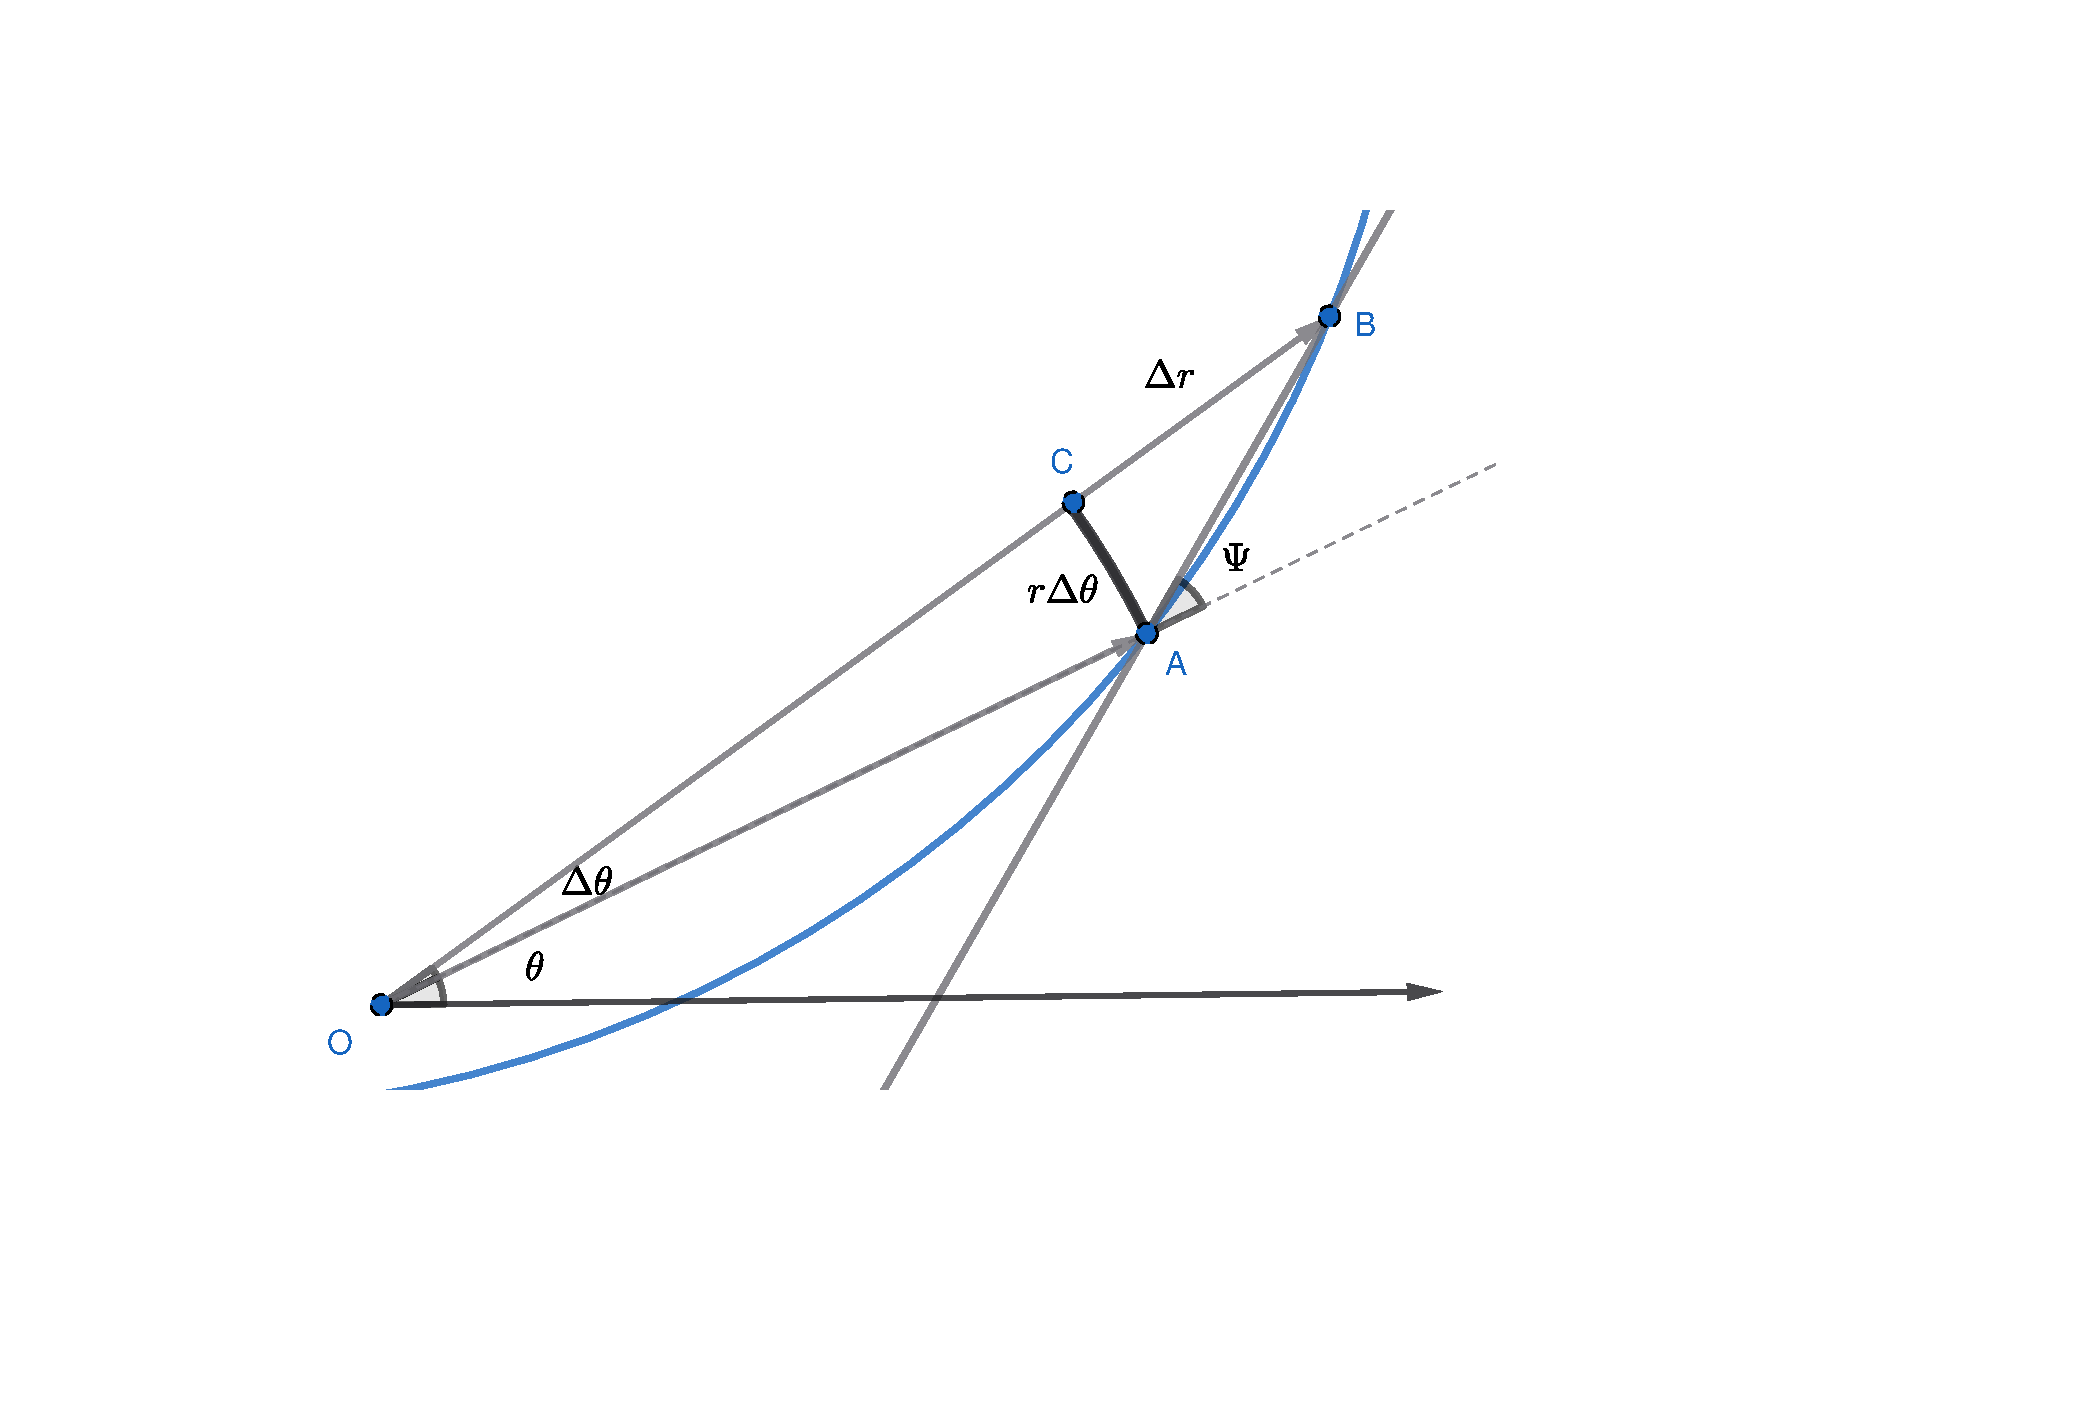
\includegraphics[scale=0.33]{img/tagent-to-r}
    \captionof{figure}{极径旋转小角度$\Delta \theta$}
  \end{center}

  \begin{proof}
如\cref{fig:tagent-to-r}所示,极径$r$旋转过一个小角度$\Delta \theta$,极径增加了$\Delta r$。小圆弧$AC$长$r\Delta \theta$,它与割线$AB$,极径的增量近似组成一个直角三角形$ACB$。当$\Delta \theta \to 0$时,点$A, B$趋向重合,割线$AB$趋近于切线。角$ABC = \Psi - \Delta \theta$

\begin{align*}
  \tan \Psi &= \lim_{\Delta \theta \to 0} \tan (\Psi - \Delta \theta) = \lim_{\Delta \theta \to 0} \tan \angle ABC \\
  &= \lim_{\Delta \theta \to 0} \frac{r\Delta \theta}{\Delta r} = \lim_{\Delta \theta \to 0} \frac{r}{\frac{\Delta r}{\Delta \theta}} \\
  &= \frac{r}{\lim_{\Delta \theta \to 0} \dfrac{\Delta r}{\Delta \theta}} = \frac{r}{r'} = \frac{ke^{b\theta}}{(ke^{b\theta})'} && \text{代入}r = ke^{\b\theta} \\
  &= \frac{ke^{b\theta}}{kbe^{b\theta}} = \frac{1}{b} && (e^{bx})' = be^{bx}
\end{align*}
是一个不依赖于$\theta$的常量,这就证明了螺线的等角性质。
  \end{proof}
}

\Question{雅各布·伯努利赞美的“虽经沧海,我依故我”也形象地描绘了求导不变$(e^x)' = e^x$的性质,现代数学家这样定义函数$f(x) = e^x$:(1) 导数不变$f'(x) = f(x)$,(2) 函数值$f(0) = 1$。试利用这个定义导出$e^x$的展开式。

\vspace{2mm}
设展开式为$f(x) = a_0 + a_1 x + a_2 x^2 + \dotsb$。由$f(0) = 1$推出:$f(0) = a_0 = 1$。求导并利用$f'(x) = f(x)$有:
\begin{align*}
f'(x) &= a_1 + 2a_2x + 3a_3x^2 + \dotsb + na_nx^{n-1} + \dotsb = f(x) \\
      &= 1 + a_1x + a_2x^2 + \dotsb + a_{n-1}x^{n-1} + \dotsb
\end{align*}
由待定系数法得:
\begin{align*}
a_1 &= 1\\
a_2 &= \frac{a_1}{2} = \frac{1}{2}\\
a_3 &= \frac{a_2}{3} = \frac{a_1}{3 \cdot 2} = \frac{1}{3!}\\
\dotso\\
a_n &= \frac{a_{n-1}}{n} = \frac{a_{n-2}}{n(n-1)} = \dotsb = \frac{1}{n!} \\
\dotso
\end{align*}

故展开式为:
\begin{align*}
e^x &= f(x) = 1 + x + \frac{x^2}{2!} + \frac{x^3}{3!} + \dotsb + \frac{x^n}{n!} + \dotsb
\end{align*}
}

\Question{*雅各布·伯努利距离发现$e^x$几乎只差一步。在计算复利时,如果年利率不是100\%,而是$x$,当$n \to \infty$时的实际年化收益率是什么?它的级数展开是什么?

\vspace{2mm}
\begin{align*}
\lim_{n \to \infty} (1 + \frac{x}{n})^n &= \lim_{n \to \infty} (1 + \frac{x}{n})^{\frac{n}{x}x} && \text{其中} x \ne 0 \\
  &= [\lim_{n' \to \infty} (1 + \frac{1}{n'})^{n'}]^x && \text{令} n' = \frac{n}{x} \\
  &= e^x
\end{align*}

利用广义二项式展开:
\begin{align*}
e^x &= \lim_{n \to \infty} (1 + \frac{x}{n})^n \\
  &= \lim_{n \to \infty} (1 + \binom{n}{1}\frac{x}{n} + \binom{n}{2}\frac{x^2}{n^2} + \dotsb \\
  &= \lim_{n \to \infty} (1 + x + \frac{n(n-1)}{2!}\frac{x^2}{n^2} + \dotsb \\
  &= \lim_{n \to \infty} (1 + x + \frac{x^2}{2!}(1-\frac{1}{n}) + \frac{x^3}{3!}(1 - \frac{1}{n})(1 - \frac{2}{n}) + \dotsb \\
  &= 1 + x + \frac{x^2}{2!} + \frac{x^3}{3!} + \dotsb
\end{align*}
}

\Question{利用复数推导三角函数的和角公式:$\tan(\theta_1 + \theta_2), \sin(\theta_1 + \theta_2), \cos(\theta_1 + \theta_2)$。

\vspace{2mm}

考虑两个复数$z_1 = a_1 + b_1i, z_1 = a_1 + b_1i$,它们的幅角分别为:$\theta_1 = \tan^{-1} \dfrac{b_1}{a_1}, \theta_2 = \tan^{-1} \dfrac{b_2}{a_2}$(忽略实部为0的情况),模为$r_1 = \sqrt{a_1^2 + b_1^2}, r_2 = \sqrt{a_2^2 + b_2^2}$。这两个复数的乘积是:

\[
z_1z_2 = (a_1 + b_1i)(a_2 + b_2i) = a_1a_2 - b_1b_2 + (a_1b_2 + b_1a_2)i
\]

根据复数的几何意义,幅角$arg(z_1z_2) = \theta_1 + \theta_2$, 模$|z_1z_2|= r_1r_2$。

\begin{align*}
\tan(\theta_1 + \theta_2) &= \tan(arg(z_1z_2)) = \frac{a_1b_2 + b_1a_2}{a_1a_2 - b_1b_2} && \text{忽略分母为0的情况} \\
  &= \frac{\frac{b_2}{a_2} + \frac{b_1}{a_1}}{1 - \frac{b_1}{a_1}\frac{b_2}{a_2}} && \text{上下同除以}a_1a_2 \\
  &= \frac{\tan\theta_2 + \tan\theta_1}{1 - \tan\theta_1 \tan\theta_2}
\end{align*}

类似地,通过$\sin(\theta_1 + \theta_2) = \dfrac{a_1b_2 + b_1a_2}{r_1r_2}$可以推出正弦、余弦的和角公式。(TODO,可展开)
}

\end{Answer}

\ifx\wholebook\relax
\chapter{代数数}
\else
\section{代数数}
\fi

\epigraph{这个世界的意义就在于理想与现实的分离。}{哥德尔}
%% "The meaning of the world is the separation of wish and fact. Wish is a force as applied to thinking beings, to realize something. A fulfilled wish is a union of wish and fact. The meaning of the whole world is the separation and the union of fact and wish". [9.4.3]
%%  Hao Wang’s supplemental biography of Gödel, A Logical Journey, MIT Press, 1996.

著名的费马大定理断言当$n \geq 3$时,$x^n + y^n = z^n$没有正整数解。尽管费马“抱怨”页边太窄,写不下他的证明,但他的确后来给出了$n=4$时$x^4 + y^4 = z^4$无解的证明。并且他还在这个过程中发展出了自己非常自豪的“无穷递降法”(Infinite descent)。在此后的200年间,数学家们一直沿着这条路摸索费马大定理的证明\citepage[40-42页]{Edward-1977}。费马发现他只需要证明如下结论就足够了\citepage[247页]{Hardy2009}。

\begin{lemma}
方程$x^4 + y^4 = z^2$没有正整数解。
\end{lemma}

的确,如果$x^4 + y^4 = u^4$有解,那么令$z = u^2$,则$x^4 + y^4 = z^2$也有解。这个引理是费马大定理$n = 4$时的充分条件。

\begin{proof}
用反证法,假设$x^4 + y^4 = z^2$有正整数解。费马进一步假设,$x, y, z$彼此互素。否则,若任何两个含有公约数$d \ne 1$,则第三个也含有这个因子(见\cref{qn:xyz-coprime}),可以从方程中约去$d$。$x^2, y^2, z$是一组勾股数,根据\cref{thm:pythagoras-triples},它们可以表示为:

\begin{align*}
x^2 &= 2mn \\
y^2 &= m^2 - n^2 \\
z &= m^2 + n^2
\end{align*}

其中$m > n$,互素且奇偶不同。上面的第二个等式可以变形为:$y^2 + n^2 = m^2$。由于$m, n$互素,所以$y, n, m$也是一组勾股数。其中$m$是奇数,$y$是奇数,$n$是偶数。再次用欧几里得引理:

\begin{align*}
n &= 2ab \\
y &= a^2 - b^2 \\
m &= a^2 + b^2
\end{align*}

其中$a > b$,互素且奇偶不同。代入$x^2 = 2mn = 4ab(a^2 + b^2)$,这说明$ab(a^2 + b^2)$是一个平方数。但$ab$与$a^2 + b^2$互素(任何素数$p$如果整除$ab$,则要么$p$整除$a$,要么整除$b$。但因为$a, b$互素,所以$p$不同时整除$a, b$,因此$p$不整除$a^2 + b^2$),所以它们也都是平方数(见\cref{qn:coprime-product-as-square})。令$a^2 + b^2 = Z^2$。因为$a, b$互素,若$ab$是平方数,则$a, b$也都是平方数。令$a = X^2, b= Y^2$,则$X^4 + Y^4 = a^2 + b^2 = Z^2$。

现在比较$X^4 + Y^4 = Z^2$与原方程$x^4 + y^4 = z^2$。它们形式一样,但:
\[
Z < Z^2 = a^2 + b^2 = m < m^2 + n^2 = z
\]

这样就能不断获得越来越小的正整数$z$,但这是不可能的。
\end{proof}

这就是无穷递降法的思路,它是一种反证法。从原来的形式$f(x)$推出同样的形式$f(X)$,但正整数$x > X > 0$。由于从任何有限的正整数开始,都不可能产生无穷递降的正整数序列,这样就可以推翻假设。\cref{fig:infinite-descent}形象地描述了无穷递降法。螺丝还有$x$圈没有拧进地面,用螺丝刀拧一阵后,还有$X$圈没有拧进地面。圈数$x > X > 0$是正整数,但螺纹的圈数有限,不可能无限拧下去。

\begin{figure}[htbp]
 \centering
 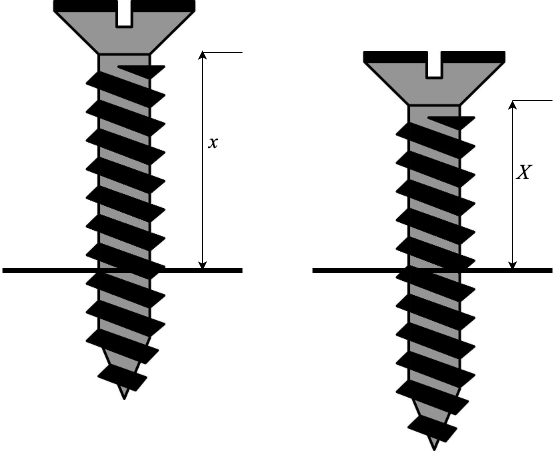
\includegraphics[scale=0.3]{img/infinite-descent}
 \caption{无穷递降法的比喻}
 \label{fig:infinite-descent}
\end{figure}

\section{费马大定理与复数}

费马之后大约一个世纪,欧拉在1755年写给哥德巴赫的信中,给出了$n = 3$时$x^3 + y^3 = z^3$没有正整数解的证明\citepage[239页]{Weil-1983}。尽管这个证明有缺陷,但欧拉本质上使用了复数攻克问题。欧拉的证明有2页,读者朋友们只要集中精神就能跟上思路,看懂并欣赏这个证明。

\begin{proof}
欧拉也使用了无穷递降法,假设$x^3 + y^3 = z^3$有解。和费马一样,他假设$x, y, z$彼此互素,并且其中有且仅有一个是偶数。首先是$x, y$是奇数,$z$是偶数的情况。此时$x \pm y$都是偶数,设$x + y = 2p, x - y = 2q$,解此二元一次方程组得:$x = p + q, y = p - q$。因为$x, y$都是奇数,所以$p, q$奇偶不同。并且因为$x, y$互素,所以$p, q$也互素(因为$p, q$的公约数$d$也整除$p \pm q$,所以也是$x, y$的公约数)。进一步,可以认为$p, q > 0$(否则交换$x, y$),这样:

\begin{align*}
z^3 &= x^3 + y^3 = (x + y)(x^2 - xy + y^2) && \text{因式分解} \\
  &= 2p[(p + q)^2 - (p + q)(p - q) + (p - q)^2] && \text{代入}x, y = p \pm q \\
  &= 2p(p^2 + q^2 + \cancel{2pq} - p^2 + q^2 + p^2 + q^2 - \cancel{2pq}) \\
  &= 2p(p^2 + 3q^2) && \text{(*)}
\end{align*}

当$z$是奇数,$x, y$一奇一偶时,欧拉也得到了同样的结果。不妨设$x$是偶数,首先移项:

\begin{align*}
x^3 &= z^3 - y^3 = (z - y)(z^2 + zy + y^2) && \text{因式分解} \\
  &= 2p[(q + p)^2 + (q + p)(q - p) + (q - p)^2] && \text{令}z \pm y = 2p, 2q \text{则}z, y = q \pm p \\
  &= 2p(p^2 + 3q^2) && \text{(**)}
\end{align*}

同样这里$p, q$是互素的正整数且奇偶不同\footnote{明显$x = -y$,是方程$x^3+ y^3 = 0$的一个解,所以$x + y$是一个因式。通过多项式长除可完成$x^3 + y^3$的因式分解。同样$z = y$,是方程$z^3 - y^3 = 0$的一个解,所以$z - y$是一个因式。通过多项式长除可完成$z^3 - y^3$的因式分解。}。接下来欧拉的思路是要证明$2p$和$p^2 + 3q^2$互素,因此它们各自是一个立方数(与费马证明$n = 4$时的思路相似)。但很可惜,它们\underdot{可能}有公因子3。例如3整除$p$,但不整除$q$,仍然满足$p, q$互素,但3此时会整除$p^2 + 3q^2$。于是欧拉分两种情况进行证明:(a) 3不能整除$p$;(b) 3整除$p$。其中(b)经过处理后可以变成(a)。接下来欧拉考虑(a),因为互素,所以$2p$和$p^2 + 3q^2$都是立方数。

现在轮到复数登场了。$i$能帮助我们把熟悉的平方差公式扩展到平方和:$a^2 + b^2 = a^2 - (-b^2) = (a + ib)(a - ib)$。这样就可以对$p^2 + 3q^2$因式分解了:

\[
p^2 + 3q^2 = (p + i\sqrt{3}q)(p - i\sqrt{3}q) = \text{立方数}
\]

接下来的做法和邦贝利类似,$p \pm i\sqrt{3}q$的乘积是立方数,它们各自是一个立方数,形如$a \pm i\sqrt{3}b$:

\begin{align*}
p + i\sqrt{3}q &= (a + i\sqrt{3}b)^3 \\
  &= a^3 + 3a^2bi\sqrt{3} + 3ab^2(-3) + b^3(-3)i\sqrt{3} && \text{二项式展开} \\
  &= a^3 - 9ab^2 + (3a^2b - 3b^3)i\sqrt{3}
\end{align*}

用待定系数法有:

\begin{align} \label{eq:Euler-gap}
p &= a^3 - 9ab^2       & q &= 3a^2b - 3b^3 \\
  &= a(a - 3b)(a + 3b) &   &= 3b(a - b)(a + b)
\end{align}

由于$p, q$互素,所以$a, b$也互素(因为任何$a, b$的公因子也是$p, q$的公因子)并且奇偶相反(否则$p, q$将都是偶数)。由于$2p$也是立方数,所以:

\[
2p = 2a(a - 3b)(a + 3b) = \text{立方数}
\]

注意到$2a, a \pm 3b$的公因子也必然是$a$和$3b$的公因子,但$a, b$互素,所以这个公因子只可能是3。但如果3整除$a$,则3也整除$p$,这与情况(a)的预设不符。这样分析下来,$2a, a \pm 3b$是彼此互素的,它们也必然都是立方数。令$2a = Z^3, a - 3b = X^3, a+ 3b = Y^3$,于是:

\[
X^3 + Y^3 = a - \cancel{3b} + a + \cancel{3b} = 2a = Z^3
\]

这样欧拉就从最初的方程$x^3 + y^3 = z^3$得到了同一形式的方程$X^3 + Y^3 = Z^3$。接下来比较$z, Z$之间的大小。$X^3Y^3Z^3 = 2a(a - 3b)(a + 3b) = 2p$,由式(*)和(**),如果$z$是偶数,则$X^3Y^3Z^3$整除$z^3$;如果$x$是偶数,则它整除$x^3$。两种情况下都有$X^3Y^3Z^3 < z^3$。如果$Z > 0$则$Z < z$;如果$Z < 0$,可以通过移项把它交换到左边,例如$X^3 + (-Z)^3 = (-Y)^3$,使得$-Y > 0$,然后把$-Y$重新命名为$Z$。经过这样的处理就得到正整数$Z < z$。使用无穷递降法就证明了情况(a)。

最后证明情况(b)。若3整除$p$,设$p = 3s$,因为$p, q$互素,所以3不能整除$q$。这样
\[
2p(p^2 + 3q^2) = 2(3s)[(3s)^2 + 3q^2] = 3^2\cdot 2s(3s^2 + q^2) = \text{立方数}
\]

容易看出$3^2\cdot 2s$和$(3s^2 + q^2)$互素,所以它们各自是一个立方数。复用(a)中的结论\cref{eq:Euler-gap},有:

\begin{align*}
q &= a(a - 3b)(a + 3b)  &  s = 3b(a - b)(a + b)
\end{align*}

其中$a, b$互素且奇偶相反。因为$3^2\cdot 2s$是立方数,而$3^2\cdot 2 \cdot 3b(a - b)(a + b) = 3^3 \cdot 2b(a - b)(a + b)$,所以$2b(a - b)(a + b)$是立方数。又由于$a, b$互素且奇偶相反,所以$2b, a \pm b$彼此互素,它们每一个都是立方数。令$2b = X^3, a - b = Y^3, a + b = Z^3$,有:

\[
X^3 + Y^3 = 2b + a - b = a + b = Z^3
\]

后面的证明就和(a)一样了:通过正整数$Z < z$得到无穷递降,导出矛盾。
\end{proof}

但欧拉的证明有一处缺陷,问题出现在\cref{eq:Euler-gap}这一步。我们屡次说因为$p, q$互素,它们的乘积$pq$是一个平方数,所以它们每个都是平方数;它们的乘积$pq$是立方数,所以每个都是立方数;它们的乘积$pq$是$n$次方数,所以每个都是$n$次方数。这个结论对于整数没有问题,因为算术基本定理保证了这一点(见\cref{qn:coprime-product-as-square})。但是欧拉一旦把它推广到复数:$(p + i\sqrt{3}q)(p - i\sqrt{3}q)$是立方数,则$p \pm i\sqrt{3}q$一定是立方数么?这个立方数会不会有别的分解方式?这个问题本质上是问:算术基本定理对复数成立么?有一个坏消息和一个好消息。好消息是,算术基本定理对于欧拉证明的特殊情形成立;坏消息是,算术基本定理在复数上可能不成立,例如:

\begin{align*}
4 &= 2 \times 2 = (1 + i\sqrt{3})(1 - i\sqrt{3}) & 6 &= 2 \times 3 = (1 + i\sqrt{5})(1 - i\sqrt{5})
\end{align*}




其中2, 3是素数,我们后面会证明$1 \pm i\sqrt{3}, 1 \pm i\sqrt{5}$也是“素数”!以事后诸葛亮的角度看,欧拉在1755年写信给哥德巴赫的时候并没有意识到这个问题,但使用他在1747年给出的一个方法可以证明如下结论:

\begin{lemma}[欧拉]
如果$a^2 + 3b^2$是一个立方数,其中$a, b$互素,则存在整数$p, q$使得$a + b\sqrt{-3} = (p + q\sqrt{-3})^3$。
\end{lemma}

\section{理想数}

1847年,在费马大定理的历史上出现了戏剧性的一幕。3月1日,数学家拉梅(Lamé,他在1839年证明了费马大定理$n = 7$时成立,见\cref{fig:Lame})在法国科学院兴奋地宣布,他找到了证明费马大定理的方法!他雄心勃勃准备近期发表完整的证明,从而终结这个困扰了数学家200多年的难题。拉梅在科学院透露了他的证明概要。像欧拉一样,他大胆地使用复数作为武器来对$x^n + y^n$进行因式分解。对于分圆方程$z^n = 1$,如果$r$是一个复数根,则:

\be \label{eq:Lame-decomposition}
x^n + y^n = (x + y)(x + ry)(x + r^2y)\dotsm(x + r^{n-1}y)
\ee

其中$n$是奇数。拉梅也许是这样推理的:根据欧拉公式和棣莫弗公式,令$r = \cos \dfrac{2\pi}{n} + i\sin \dfrac{2\pi}{n}$,则方程$X^n - 1 = 0$有$n$个不同的复数根$1, r, r^2, \dotsc, r^{n-1}$,因而多项式$X^n - 1$可因式分解为$X^n - 1 = (X - 1)(X - r)(X - r^2)\dotsm(X - r^{n-1})$。令$X = -\dfrac{x}{y}$,然后两边同乘以$-y^n$就得到了\cref{eq:Lame-decomposition}。接下来拉梅打算证明,如果$x, y$互素,则所有因子$x + y, x + ry, \dotsc, x + r^{n-1}y$彼此互素。而如果$x^n + y^n = z^n$,即这些互素因子的乘积是一个$n$次方数,则每个因子也必然是$n$次方数。由此可以构造出无穷递降的正整数,从而推翻假设,完成证明。

\begin{figure}[htbp]
 \centering
 \subcaptionbox{拉梅\label{fig:Lame}}{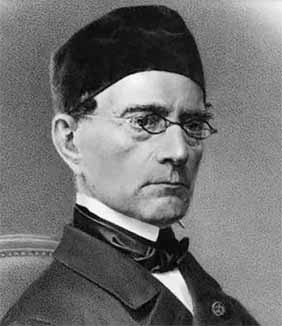
\includegraphics[scale=0.4]{img/lame}}
 \subcaptionbox{柯西\label{fig:Cauchy}}{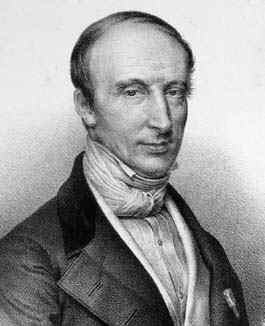
\includegraphics[scale=0.4]{img/Cauchy}}
 \caption{拉梅与柯西}
\end{figure}

在科学院成员狐疑与惊讶的眼神中,拉梅看了一眼台下的数学家刘维尔(见\cref{fig:Liouville})说,我不能独占这个荣誉。在几个月前的一次闲谈中,刘维尔提出了这个绝妙的想法。拉梅结束了他的发言后,在一片掌声与悄悄议论中,刘维尔走上讲台。他并没有表现出拉梅那样的热情,谦虚地说使用复数来解决数论问题并不是他的原创——欧拉、拉格朗日、高斯、柯西,最重要的雅可比,都曾这样使用复数。他给拉梅泼了冷水,指出很多数学家刚开始都会这么想。这个想法的关键在于,一个整数是否可以\underdot{唯一}分解为素因子的积。尽管对于普通的整数成立,但没有充分证据表明可以把这个方法推广到复数上去。

接下来轮到柯西(见\cref{fig:Cauchy})发言了。他表示拉梅有可能成功,但接着话锋一转,指出他自己早在1846年10月就向科学院提交了证明费马大定理的想法,只是他还没有来得及把证明细化。这相当于公开向拉梅挑战,看看谁能先完成费马大定理的证明。拉梅一点也不含糊,接下来的数周,他和柯西唇枪舌剑展开竞争。拉梅承认刘维尔的批评有道理,但他坚信自己的结论是正确的。他展示了迄今为止试过的所有例子都支持复数上的唯一分解,并准备证明这一“引理”。在法国科学院3月15日的会议上,数学家旺策尔\footnote{旺策尔证明了高斯——旺策尔定理,彻底解决了正多边形作图问题、三分角和倍立方问题。}宣布他“证明”了唯一分解定理在复数上的有效性,而事实上他只覆盖了$n \leq 4$的情形,接着就说“显而易见”,我们可以用类似的方法证明$n > 4$的情形。但大家包括柯西并不觉得“显而易见”。柯西于是发表了一系列论文,试图证明复数上带余数的除法,并由此证明唯一分解定理。

3月22日,柯西和拉梅的竞争达到了白热化。双方各自向科学院提交了“时间胶囊”——这是法国科学院建立的一种制度,可能是吸取了当年牛顿与莱布尼茨争夺微积分优先权的教训。双方可以把自己的想法密封后提交给科学院保存。科学院确保这些内容不会泄漏,同时学者们可以继续完善研究,并在未来产生优先权争议时进行仲裁。此后柯西和拉梅就不时在科学院公布自己的进展,似乎总是“几乎”要解决了,但还有一个“小”问题。转折发生在5月24日。刘维尔在科学院宣读了来自德国布雷斯劳的数学家库默尔(见\cref{fig:Kummer})的信。库默尔肯定了刘维尔对唯一分解定理的质疑,并附上了一份他三年前发表的论文,文中推翻了复数上的唯一分解定理。这冰冷的事实终结了拉梅与柯西的竞争。

\begin{figure}[htbp]
 \centering
 \subcaptionbox{库默尔\label{fig:Kummer}}{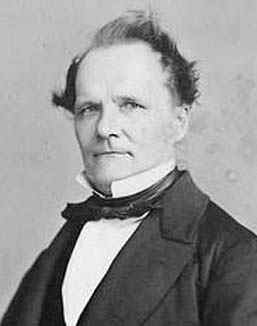
\includegraphics[scale=0.4]{img/Kummer}}
 \subcaptionbox{刘维尔\label{fig:Liouville}}{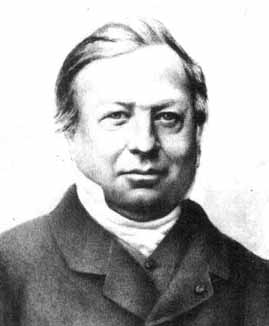
\includegraphics[scale=0.4]{img/liouville}}
 \caption{库默尔与刘维尔}
\end{figure}

但是——戏剧性的事件总有但是,库默尔说他有办法“挽救”唯一分解定理,他引入了一种称为“理想复数”(简称理想数)的新概念,可以通过理想数的唯一分解证明费马大定理。但是——又是但是,对某些特别奇怪的素数$p$,例如37,理想数也不存在。他已经找到了判断奇特素数的方法,这些成果已于一年前发表在柏林科学院。库默尔接着一举证明了费马大定理对100以内所有的素数$p$,除了37, 59, 69之外,都成立,即$x^p + y^p = z^p$无正整数解\footnote{确切地说,库默尔证明了对于所有奇素数$p$,如果$p$不整除任何伯努利数$B_2, B_4, \dotsc, B_{p-3}$的分子,则费马大定理对指数$p$成立。这样的素数叫做“正则”素数。其中伯努利数的递归定义为:$B_0 = 1$,对任意正整数$n$满足$\displaystyle \sum_{k = 0}^{n}\binom{n + 1}{k} B_k = 0$}。这不但是怀尔斯之前的最好结果,而且还开辟了一个数学新领域——代数数论。

\begin{mdframed}
库默尔简介
\end{mdframed}

\section{高斯整数}

要想把整除、素数等概念扩展到复数,首先必须定义什么是“复整数”。最直观的一个想法是扩展成$a + bi$,其中$a, b$是整数。但这还不够,我们看到欧拉似乎把$a + i\sqrt{3}b$看成整数。从历史经验看,方程是发现探索“未知数”的有力武器。通过解一次方程$ax = b$,我们认识到有理数$x = \frac{b}{a}$;通过解二次方程,我们认识到无理数;通过解三次方程,我们认识到复数;通过解高次方程,我们认识到有无法用根式表示的数。通过代数基本定理,我们认识到那些无法用根式表示的数也都是复数,它们可以用代数方程定义:

\[
a_n x^n + a_{n-1} x^{n-1} + \dotsb + a_1 x + a_0 = 0
\]

其中$a_n, a_{n-1}, ..., a_1, a_0$是整数。为什么系数不是有理数呢?假设它们是有理数$a_i = \frac{b_i}{c_i}$,两边乘以分母的最小公倍数,我们就把系数变回了整数。所以系数是整数就足够了。厄米特和林德曼分别证明了$\pi, e$不是这样的代数方程的解。为了加以区分,我们把满足代数方程的数叫做代数数(algebraic number),否则叫做超越数(transcendent number),$\pi, e$都是超越数。代数数的定义是抽象的、间接的。和$1 + i\sqrt{2}$不同,我们没有给出代数数的表达式,它们是代数方程的解,存在那里,但可能没法用根式表达。按照这个定义,当$n = 1$时,方程是一次方程$ax + b = 0$,解$x = \frac{b}{a}$。如果系数$a = 1$,则$x$是整数;受此启发,我们定义$a_n = 1$时,代数方程:

\[
x^n + a_{n-1} x^{n-1} + \dotsb + a_1 x + a_0 = 0
\]

的解叫做代数整数(algebraic integer),这样的方程叫做“首一方程”(monic equation)。代数整数既包括普通的整数(又叫有理整数rational integer,见\cref{qn:rational-solution-is-integral}),也包括了更复杂的整数。为了避免胡子眉毛一把抓,我们从最简单的二次首一方程开始探索代数整数。当一次项是偶数时,方程$x^2 - 2ax + a^2 + b^2 = 0$的解是$a \pm bi$。高斯最早对这种形式的数进行研究,今天我们把这种数叫做“高斯整数”,用记号$\mathbb{Z}[i]$表示,这个记号暗示了我们把虚数单位$i$加入到整数$\mathbb{Z}$中\footnote{符号$\mathbb{Z}[x]$叫做整数环$\mathbb{Z}$上的一元多项式,它由形如$a_n x^n + a_{n-1} x^{n-1} + \dotsb + a_1 x + a_0$的元素组成,其中$a_0, a_1, \dotsc, a_n \in \mathbb{Z}$是整数。}。

为了区分代数整数和普通有理整数,我们用希腊字母$\alpha, \beta, \gamma, \dotsc$表示代数整数,用英文字母$a, b, c, \dotsc$表示有理整数(附录\ref{ch:greek-letters}有希腊字母的读音)。和普通整数类似,我们很容易验证高斯整数之间的$+, -, \times$运算结果仍然是高斯整数,但除法不一定(正如同普通有理整数之间的除法结果不一定是有理整数)。利用这一点就能定义整除了。如果高斯整数$\alpha = \beta\gamma$是另外两个高斯整数的积,我们称$\beta$整除$\alpha$。接下来的问题有些棘手:(1) 怎样定义带余数的除法?(2) 怎样定义高斯整数中的素数?

带余数的除法需要“更小”这一概念,普通有理整数带余数的除法是$a = bq + r$,其中$r < b$,即余数比除数“更小”。但是复数本质上是向量,不能直接比较大小。例如我们不能说$1 + i$“小于”2。只有复数的模是可以比较大小的,例如$|1 + i| = \sqrt{1^2 + 1^2} = \sqrt{2} < 2 = |2|$。为了解决什么是“更小”的问题,高斯于1832年定义了一个重要的概念:范数(Norm),复数$z = a + bi$的范数为:

\[
N(z) = a^2 + b^2
\]

它实际是模的平方,因而总是$\geq 0$,并且和共轭复数有不解之缘:

\[
N(z) = a^2 + b^2 = z\overline{z} = N(\overline{z})
\]

范数和模一样,是可乘的(见\cref{qn:norm-is-multiplicative}):

\[
N(\alpha\beta) = N(\alpha)N(\beta)
\]

利用范数,高斯扩展了1的概念。在普通有理整数中,$3 = 3 \times 1$。一旦考虑负整数,情况就丰富起来:$-3 = 3 \times (-1) = -3 \times 1$。但取绝对值的话,情况就统一到:$|3| = |(\pm 3) \times (\pm 1)| = 3 \times 1$。高斯定义范数$N(\mu) = 1$的数是单位元(unit),若$\alpha = \mu \alpha'$,称$\alpha'$是$\alpha$的“相伴元”(associate,英文关联的意思)。这样在上述有理整数的例子中,$-1, 1$都是单位元,而-3和3是相伴的。扩展到高斯整数,单位元有4个:
%% 由$N(\mu) = a^2 + b^2 = 1$,其中$a, b \in \mathbb{Z}$是整数,要么$a^2 = 1, b^2 = 0$,要么$a^2 = 0, b^2 = 1$。分别对应$a = \pm 1, b = 0$和$a = 0, b = \pm 1$,
$\pm 1, \pm i$。例如$1 + i = (1 - i)i$,因为$|i| = 1$是单位元,所以$1 + i$和$1 - i$是相伴的,如同普通有理整数中相伴的$\pm 3$。单位元还有一个等价的定义:凡是整除1的数叫做单位元。这样$\mu^n = 1$,有趣的是,有理整数的两个单位元分别是$(-1)^0, (-1)^1$;而高斯整数的4个单位元分别是$i^{0, 1, 2, 3}$次幂。读者朋友们,你是否想到了分圆方程?
%% 分圆方程的根是单位元吗?

范数一举扫清了带余数除法的障碍:一个直观的想法是用高斯整数的$N(\gamma) < N(\beta)$来代替有理整数的$r < b$。这样高斯整数带余数的除法就可定义为:

\begin{align*}
\alpha &= \rho \beta + \gamma & \text{其中} \beta &\ne 0, N(\gamma) < N(\beta)
\end{align*}

但是且慢,给定被除数$\alpha$和除数$\beta$,商$\rho$和余数$\gamma$一定存在么?如果不存在,这个定义就站不住脚了。于是高斯接下来证明了:

\begin{theorem}
给定高斯整数$\alpha$和$\beta \ne 0$,存在高斯整数$\rho, \gamma$使得$\alpha = \rho \beta + \gamma$,其中$N(\gamma) < N(\beta)$。
\end{theorem}

\begin{proof}
令$\rho = m + ni$,其中$m, n$是有理整数,所有$\rho \beta$都可写为:

\[
\rho \beta = (m + ni)\beta = m\beta + ni\beta
\]

即复数$\beta$的倍数和$i\beta$的倍数的和。在几何上$i\beta$相当于向量$\beta$旋转90度(见\cref{qn:mul-i})。如\cref{fig:zi}所示,$i\beta$与$\beta$垂直。因此所有的$\rho \beta$分布在边长为$|\beta|$的方格子的交点上。

\begin{figure}[htbp]
 \centering
 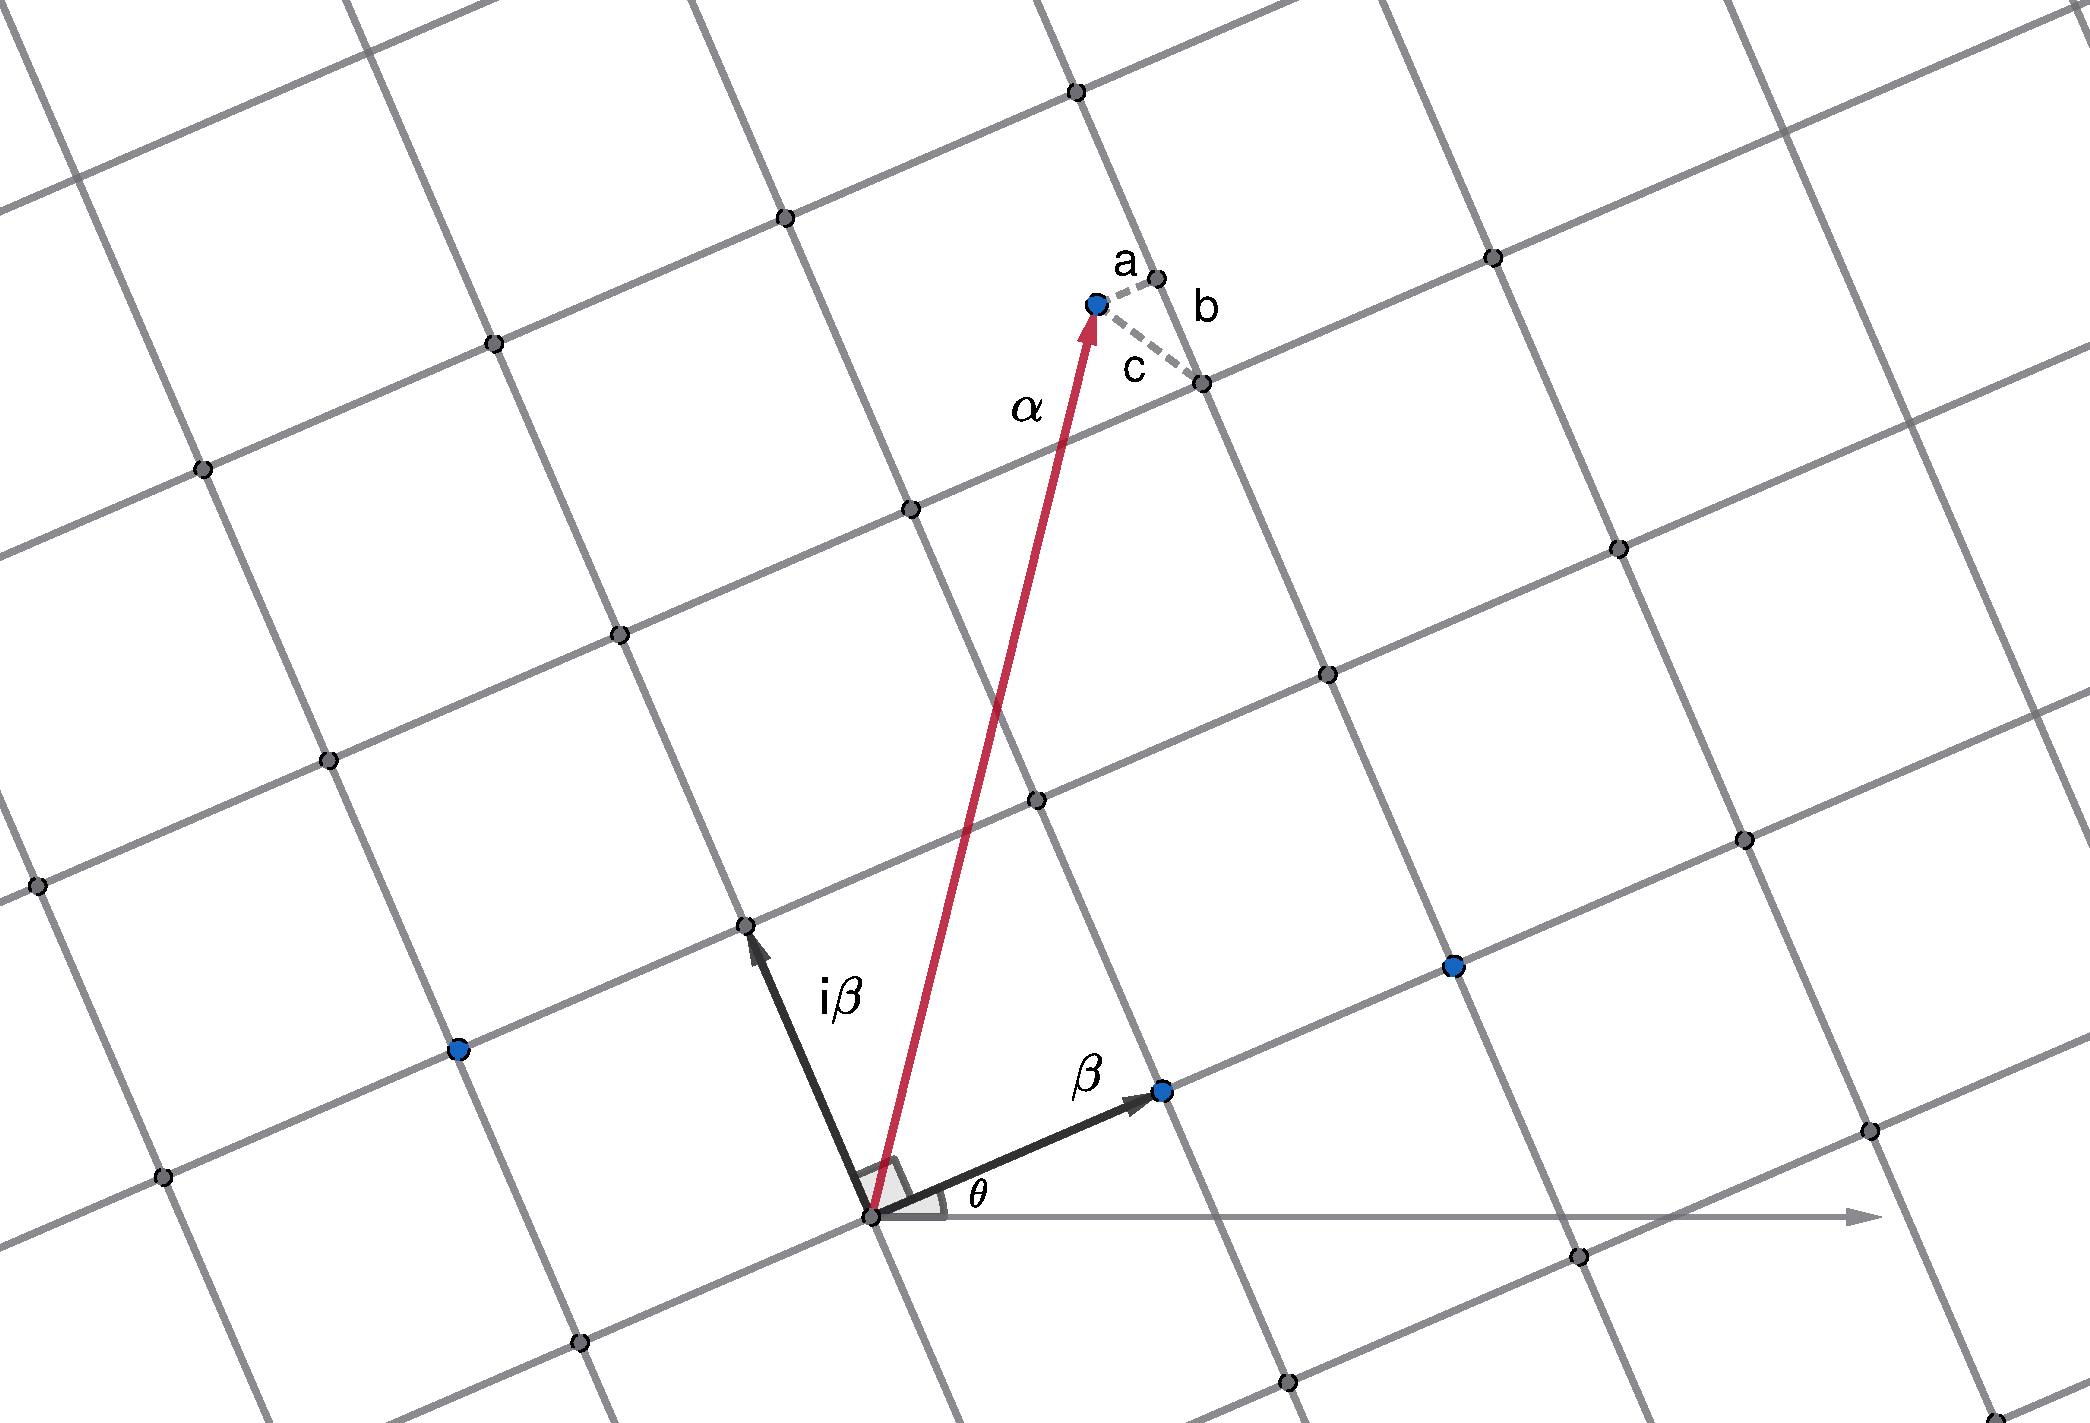
\includegraphics[scale=0.3]{img/zi}
 \caption{高斯整数$\rho \beta$的所有值构成一个网格,$\alpha$落在某个格子中。}
 \label{fig:zi}
\end{figure}

被除数$\alpha$所代表的向量必然落在某个格子中(包括边)。它到最近的两个边的距离都$\leq \frac{|\beta|}{2}$(如\cref{fig:zi}中$a, b \leq \frac{|\beta|}{2}$)。由三角形两边和大于第三边,有:

\[
|\gamma| = |c| < |a| + |b| \leq \frac{|\beta|}{2} + \frac{|\beta|}{2} = |\beta|
\]
两边平方得$N(\gamma) < N(\beta)$。
\end{proof}

有了带余数除法,就意味着可以使用欧几里得算法了(见第\ref{sec:Euclidean-algorithm}节)。高斯把欧几里得算法扩展到高斯整数。

\begin{align*}
\alpha   &= \rho_1 \beta + \gamma_1    & N(\gamma_1) &< N(\beta) \\
\beta    &= \rho_2 \gamma_1 + \gamma_2 & N(\gamma_2) &< N(\gamma_1) \\
\gamma_1 &= \rho_3 \gamma_2 + \gamma_3 & N(\gamma_3) &< N(\gamma_2) \\
         & \dotso
\end{align*}

但这个过程不会永远进行下去,因为范数是普通的非负整数,所以必然存在某个$n$使得$N(\beta) > N(\gamma_1) > N(\gamma_2) > \dotsb > N(\gamma_n) > N(\gamma_{n+1})= 0$。即:

\begin{align*}
\gamma_{n-2} &= \rho_n \gamma_{n-1} + \gamma_n & N(\gamma_n) &< N(\gamma_{n-1}) \\
\gamma_{n-1} &= \rho_{n+1} \gamma_n
\end{align*}

这样$\gamma_n$整除$\gamma_{n-1} \to$整除$\gamma_{n-2} \to \dotsb \to$整除$\beta \to$整除$\alpha$。所以$\gamma_n$是$\alpha, \beta$的公约数。反之,任何$\alpha, \beta$的公约数$\psi$必然整除$\alpha \to$整除$\beta \to$整除$\gamma_1 \to$整除$\gamma_2 \to \dotsb \to$整除$\gamma_n$。因此$\gamma_n = (\alpha, \beta)$是\underdot{最大}公约数\footnote{这里对应的英文是highest common divisor而不是greatest common divisor,因为复数不能直接比较大小。}。我们给最大两个字加了点是因为:(1) 复数不能直接比较大小,这里“最大”的涵义是,任何公约数$\psi$都整除$\gamma_n$。(2) 高斯整数的最大公约数不唯一。如果一个数乘以单位元$\mu\phi = \gamma_n$,则$\phi$也是最大公约数。例如$3 + i$与$1 + 3i$的最大公约数是$-1 + i$,它乘以$-1, \pm i$得到的相伴元$1 - i, i(-1 + i) = -1 - i, -i(-1 + i) = 1 + i$也都是最大公约数。

接下来高斯要回答什么才是素数。一旦引入复数,普通的素数$2, 3, 5, 7, \dotsc$中,有些竟然可以分解,如:$2 = (1 + i)(1 - i), 5 = (2 + i)(2 - i)$。而素数的直观涵义是“基础砖石”,它们能构成其它整数而自己不能被进一步分解。可是究竟什么是“进一步”呢?例如$1 + i = (1 - i)i$,我们此时立即看出高斯定义单位元和相伴元的意义了。如果一个数只能分解为相伴元和单位元的乘积,这不是“进一步”,而是“原地踏步”。于是高斯给出了素数的扩展定义:

\begin{definition}
一个高斯整数是素数如果它不等于0或任何单位元,并且只能被和它相伴的数与单位元整除。
\end{definition}

我们通常用字母$p$表示普通有理整数中的素数,用希腊字母$\pi$来表示代数整数中的素数。注意不要和圆周率混淆。在高斯整数中,一个素数$\pi$有8个因子:$\pm 1, \pm i, \pm \pi, \pm i\pi$。接下来的问题是如何找到这些素数?

\begin{proposition}\label{thm:prime-norm}
如果一个高斯整数$\psi$的范数是有理素数$p$,则$\psi$是高斯素数。
\end{proposition}

\begin{proof}
假设$\psi = \alpha\beta$是两个高斯整数的积,两边取范数:

\begin{align*}
p &= N(\psi) = N(\alpha\beta) = N(\alpha)N(\beta)  && \text{范数可乘}
\end{align*}

有理素数的因子只有$1, p$。所以$N(\alpha)$和$N(\beta)$中必然有一个是1,因而是单位元。另外一个必然和$\psi$相伴,由定义知$\psi$是高斯素数。
\end{proof}

根据这个结论,我们马上可以判断$1 \pm i, 2 \pm i, 1 \pm 2i$都是素数(它们的范数$N(1 \pm i) = 1^2 + 1^2 = 2, N(2 \pm i) = N(1 \pm 2i) = 1^2 + 2^2 = 5$都是有理素数)。但这个命题的逆命题不成立,高斯素数的范数并不一定是有理素数。例如$N(3) = 9$,不是有理素数,假设3可以分成两个高斯整数的积$3 = (a + bi)(c + di)$。两边取范数:

\[
9 = N(3) = N(a + bi)N(c + di) = (a^2 + b^2)(c^2 + d^2)
\]

很容易验证3不是两个正整数的平方和(3只有一种正整数分解:3 = 2 + 1,其中2不是平方数),因此$a^2 + b^2 = c^2 + d^2 = 3$是不可能的。这样$a^2 + b^2$和$c^2 + d^2$只能是1和9。不管哪个是1,其对应的高斯整数是一个单位元。因此根据定义,3是高斯素数。这提示我们,如果一个有理素数$p$能表示为两个正整数的平方和$p = a^2 + b^2$,则它可分解为$p = (a + bi)(a - bi)$因而不是素数;反之,如果$p$不能表示为平方和,使用类似的推理,假设$p = (a + bi)(c + di)$,取范数:

\[
p^2 = N(p) = N(a + bi)N(c + di) = (a^2 + b^2)(c^2 + d^2)
\]

因为$p$不是平方和,所以不可$a^2 + b^2 = c^2 + d^2 = p$;故$a^2 + b^2$和$c^2 + d^2$只能是1和$p^2$。不管哪个是1,其对应的高斯整数是单位元,所以$p$是高斯素数。有理素数中只有2是偶数。因为$2 = 1^2 + 1^2$,所以$2 = (1 + i)(1 - i)$不是高斯素数。我们此前已经判断出$1 \pm i$及其相伴元都是素数。剩下的所有奇素数可分为两类:形如$4n + 3$的和形如$4n + 1$的。例如3就是前一类,我们怀疑$4n + 3$形的素数不能拆成平方和,幸运地是我们猜对了。

\begin{proposition}
形如$4n + 3$的奇素数不能表示成正整数的平方和。
\end{proposition}

\begin{proof}
用反证法,假设$a^2 + b^2 = 4n + 3$。$a, b$的奇偶必然不同,否则它们的平方和是偶数。不妨令$a = 2k + 1, b = 2m$,有:

\[
a^2 + b^2 = (2k + 1)^2 + (2m)^2 = 4k^2 + 4k + 1 + 4m^2 = 4(k^2 + k + m^2) + 1
\]

是$4n + 1$的形式而不是$4n + 3$的形式,矛盾。
\end{proof}

这样,所有$3, 7, 11, \dotsc$都是高斯素数了。为了处理$4n + 1$形的素数,我们需要一个重要的武器:高斯整数上的算术基本定理。我们的思路和第\ref{sec:fundamental-theorem-of-arithmetic}节一样:通过高斯整数上的欧几里得算法推出算术基本定理。

\begin{proposition}
如果高斯整数$\alpha, \beta$互素,即$(\alpha, \beta) = 1$,并且$\alpha$整除乘积$\beta \psi$,则$\alpha$整除$\psi$。
\end{proposition}

\begin{proof}
把欧几里得算法中的数都放大$\psi$倍,最后得:

\begin{align*}
(\alpha \psi, \beta \psi) &= \gamma_n \psi = \psi  && \text{由} 1 = (\alpha, \beta) = \gamma_n
\end{align*}

即最大公约数是$\psi$。如果$\alpha$整除$\beta \psi$,由于$\alpha$也整除$\alpha \psi$,因此$\alpha$是公约数,它必然整除最大公约数$\psi$。
\end{proof}

\begin{corollary}\label{thm:Gaussian-primary}
如果高斯素数$\pi$整除乘积$\alpha \beta$,则$\pi$整除$\alpha$或$\pi$整除$\beta$。
\end{corollary}

\begin{proof}
如果素数$\pi$不整除$\alpha$,则$(\pi, \alpha) = 1$。若$\pi$整除$\alpha \beta$,据上面的命题,$\pi$整除$\beta$。
\end{proof}

利用这个推论就可以证明高斯整数上的算术基本定理了。

\begin{theorem}[高斯整数上的算术基本定理]
高斯整数可以唯一分解为高斯素数的乘积,如果不考虑这些素数的顺序、相伴元、有否单位元的话。
\end{theorem}

\begin{proof}
用反证法,假设某一高斯整数有两种高斯素数分解:
\[
\pi_1 \pi_2 \dotsm \pi_j = \psi_1 \psi_2 \dotsm \psi_k
\]
其中某个素因子$\pi_i$既不是单位元,也不与右侧任何素因子相伴。根据上述推论,因为素数$\pi_i$整除彼此互素数的积$\psi_1 \psi_2 \dotsm \psi_k$,所以$\pi_i$要么整除$\psi_1$,要么整除$\psi_2, \dotsc, $要么整除$\psi_k$。但这是不可能的,因为每个素数$\psi_1, \psi_2, \dotsc, \psi_k$都不可能被不相伴的数整除。因此假设不成立,任何高斯整数只有一种高斯素数分解。
\end{proof}

现在我们可以调转枪头,分拆$4n + 1$形的有理素数,从而彻底解决高斯素数问题。我们需要用到初等数论中的威尔逊定理(见附录\ref{app:wilsons-theorem}):如果$p$是素数,则阶乘$(p - 1)! \equiv -1 \pmod p$。

\begin{lemma}
存在某个平方和$x^2 + 1$能被形如$p = 4n + 1$的有理素数整除。
\end{lemma}

\begin{proof}
$p = 4n + 1$,阶乘$(p - 1)!$包含$4n = 2n + 2n$项:
\begin{align*}
(p - 1)! &= 1 \cdot 2  \dotsm  2n \cdot (2n + 1)  \dotsm  4n \\
  &= (1 \cdot 2  \dotsm  2n)[(p - 1) \cdot (p - 2)  \dotsm  (p - 2n)] && \text{反转后半段} \\
  &\equiv (1 \cdot 2  \dotsm 2n)(-1 \cdot -2 \dotsm -2n) \pmod p && \text{由} p - k \equiv k \pmod p \\
  &\equiv (2n)!(-1)^{2n}(2n)! = [(2n)!]^2 = x^2 \pmod p && \text{令} x = (2n)!
\end{align*}
另一方面,由威尔逊定理有$(p - 1)! \equiv -1 \pmod p$。所以$x^2 \equiv -1 \pmod p$,即$p$整除某个$x^2 + 1$。
\end{proof}

现在$p = 4n + 1$整除某个$x^2 + 1 = (x + i)(x - i)$。如果$p$也是高斯素数,则$p$整除$x + i$或$x - i$(据推论\ref{thm:Gaussian-primary})。但是$\dfrac{x}{p} \pm \dfrac{1}{p}i$不可能是高斯整数。这个矛盾说明$p$不是高斯素数,因而必然能分解为乘积:$p = (a + bi)(c + di)$,其中$a + bi$和$c + di$都不是单位元($a^2 + b^2 \ne 1 \ne c^2 + d^2$)。两边取范数:

\[
p^2 = N(p) = N(a+bi)N(c+di) = (a^2 + b^2)(c^2 + d^2)
\]

因此只能是$a^2 + b^2 = c^2 + d^2 = p$。另一方面如果$p = a^2 + b^2 = (a + bi)(a - bi)$。由于$N(a \pm bi) = p$,根据命题\ref{thm:prime-norm},它们都是高斯素数。接着根据高斯整数的算术基本定理,这种分解是\underdot{唯一}的。所以必然有$a^2 = c^2, b^2 = d^2$。这样我们就解决了$4n + 1$形的素数,并且利用高斯整数证明了如下结论\footnote{1640年12月25日,费马在给梅森的信中提出了这一命题。费马曾多次告诉友人,他用无穷递降法证明了这个猜想,但一直未发现相关的文献资料。一个多世纪后,欧拉在1754年首次给出了该命题的证明。}:

\begin{theorem}[费马平方和定理]
有理素数$p = 4n + 1$一定可以分解为两个平方和$a^2 + b^2$。
\end{theorem}

我们用下面的定理总结上述三种情况:(1) 唯一的偶素数$p = 2$;(2) 形如$4n + 3$的奇素数;(3) 形如$4n + 1$的即素数。

\begin{theorem}
高斯素数包括三种:(1) $1 + i$及其相伴元;(2) 有理素数$4n + 3$及其相伴元;(3) 有理素数$4n + 1$的因子$a + bi$。
\end{theorem}

\begin{mdframed}
高斯简介
\end{mdframed}

\section{二次整数}

高斯整数是二次首一代数方程中最简单的情况。稍微改变一下方程,$x^2 - 2ax + (a^2 + mb^2) = 0$的解是$a \pm b\sqrt{-m}$,其中$m$不含任何平方因子。这种形式的代数整数,是二次方程的解,叫做“二次整数”,用$\mathbb{Z}[\sqrt{-m}]$表示。例如$\mathbb{Z}[\sqrt{-2}], \mathbb{Z}[\sqrt{-3}]$等。我们由此看出欧拉在证明费马大定理$n=3$时的分解:

\[
p^2 + 3q^2 = (p + q\sqrt{-3})(q - q\sqrt{-3})
\]

是关于二次整数$\mathbb{Z}[\sqrt{-3}]$的。高斯对$\mathbb{Z}[i]$的处理为我们树立了样板:(a) 先定义范数,(b) 然后扩展欧几里得算法,(c) 找出素数。我们先从$\mathbb{Z}[\sqrt{-2}]$开始热身一下。受共轭复数的启发,我们扩展范数的定义如下:

\begin{definition}
二次整数$\xi = a + b\sqrt{-m}$的范数定义为$N(\xi) = \xi\overline{\xi} = (a + b\sqrt{-m})(a - b\sqrt{-m}) = a^2 + mb^2$
\end{definition}

注意到这恰好是二次方程的常数项,这并非巧合(见\cref{qn:quadratic-norm})。对于$\mathbb{Z}[\sqrt{-2}]$,范数为$a^2 + 2b^2$。单位元是
%% 的范数为1,只可能是$a^2 = 1, b = 0$,即
$\mu = \pm 1$。接下来我们判断$\mathbb{Z}[\sqrt{-2}]$上是否有欧几里得算法。也就是说,任给整数$\alpha, \beta \ne 0$,是否存在整数$\rho, \gamma$使得$\alpha = \rho \beta + \gamma$,并且$N(\gamma) < N(\beta)$。令$\rho = m + n\sqrt{-2}$,则$\rho \beta = m\beta + n\sqrt{-2}\beta$,它是由向量$\beta$和$i\sqrt{2}\beta$张成的矩形网格,如\cref{fig:Z-sqrt-2}所示。因为$i\sqrt{2}\beta$把$\beta$旋转90度后放大$\sqrt{2}$倍,所以矩形的宽是$|\beta|$长是$\sqrt{2}|\beta|$。任何整数$\alpha$都落在某个矩形中,它距离最近的顶点距离的平方可由勾股定理得到:

\begin{figure}[htbp]
 \centering
 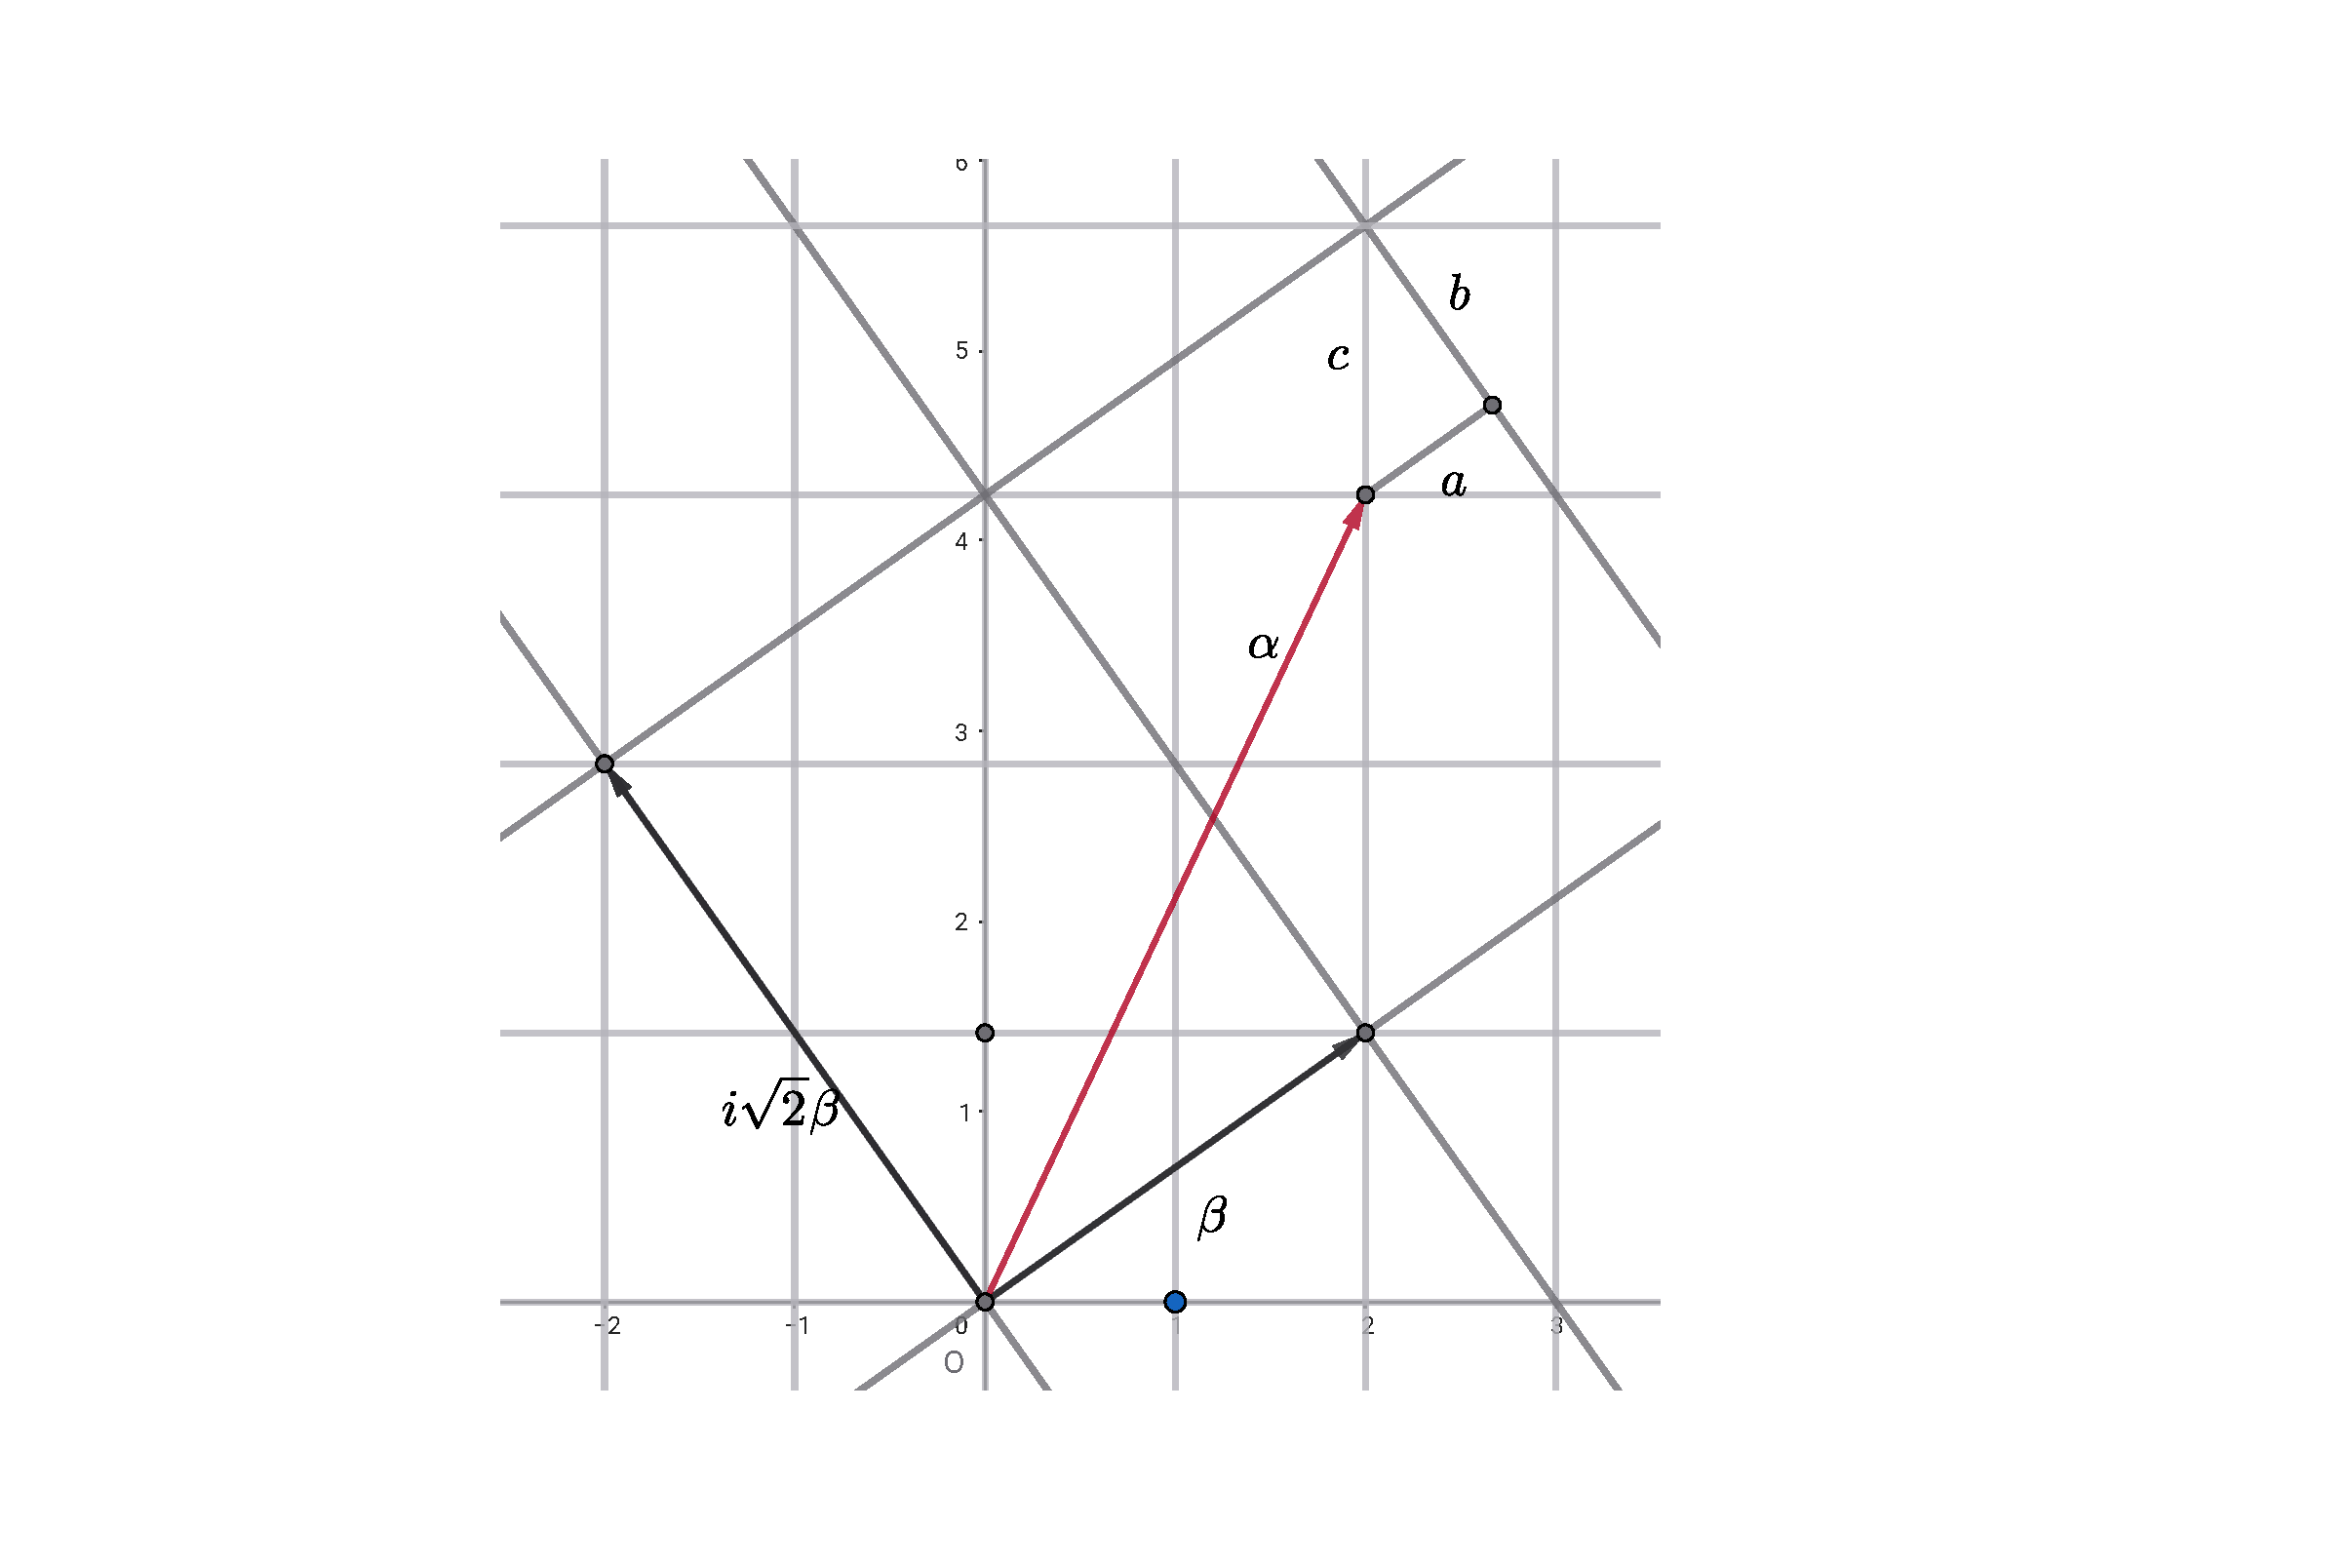
\includegraphics[scale=0.3]{img/z-sqrt-2}
 \caption{$\mathbb{Z}[\sqrt{-2}]$中的整数构成浅灰色网格,积$\rho \beta$构成黑色网格,$\alpha$落在某个格子中。}
 \label{fig:Z-sqrt-2}
\end{figure}

\begin{align*}
N(\alpha - \rho\beta) & = c^2 = a^2 + b^2  && \text{勾股定理} \\
  &\leq (\frac{\sqrt{2}}{2}|\beta|)^2 + (\frac{1}{2}|\beta|)^2 && a, b\text{都不大于矩形边长的一半} \\
  &= \frac{3}{4}|\beta|^2 < |\beta|^2 = N(\beta)
\end{align*}

令$\gamma = \alpha - \rho \beta$即可。这样欧几里得算法在$\mathbb{Z}[\sqrt{-2}]$上也成立,从而算术基本定理也成立。但接下来的$\mathbb{Z}[\sqrt{-3}]$却让人失望了。因为存在这样的反例:

\[
4 = 2 \times 2 = (1 + i\sqrt{3})(1 - i\sqrt{3})
\]

其中2不能被进一步分解,否则假设$2 = (a + b\sqrt{-3})(c + d\sqrt{-3})$,两边取范数:

\[
4 = N(2) = N(a+b\sqrt{-3})N(c + d\sqrt{-3}) = (a^2 + 3b^2)(c^2 + 3d^2)
\]

不可能$a^2 + 3b^2 = c^2 + 3d^2 = 2$,这个方程没有整数解。所以$a^2 + 3b^2$或$c^2 + 3d^2$是1,其对应的是单位元,另一个是2的相伴元。这就证明了2不能被分解。$1 \pm i\sqrt{3}$的范数都是4,通过同样的分析,我们知道它们也不能被分解。这样4就有两种分解方式。这是为什么呢?如\ref{fig:Z-sqrt-3}所示,所有$\rho \beta$是由$\beta$和$i\sqrt{3}\beta$张成的矩形网格。任何$\alpha$落在某个矩形中,它距离最近的顶点距离的平方是:

\begin{align*}
N(\alpha - \rho \beta) &= c^2 = a^2 + b^2  && \text{勾股定理} \\
  &\leq (\frac{\sqrt{3}}{2}|\beta|)^2 + (\frac{1}{2}|\beta|)^2 = |\beta|^2 && a, b \leq \text{长宽的一半}
\end{align*}

\begin{figure}[htbp]
 \centering
 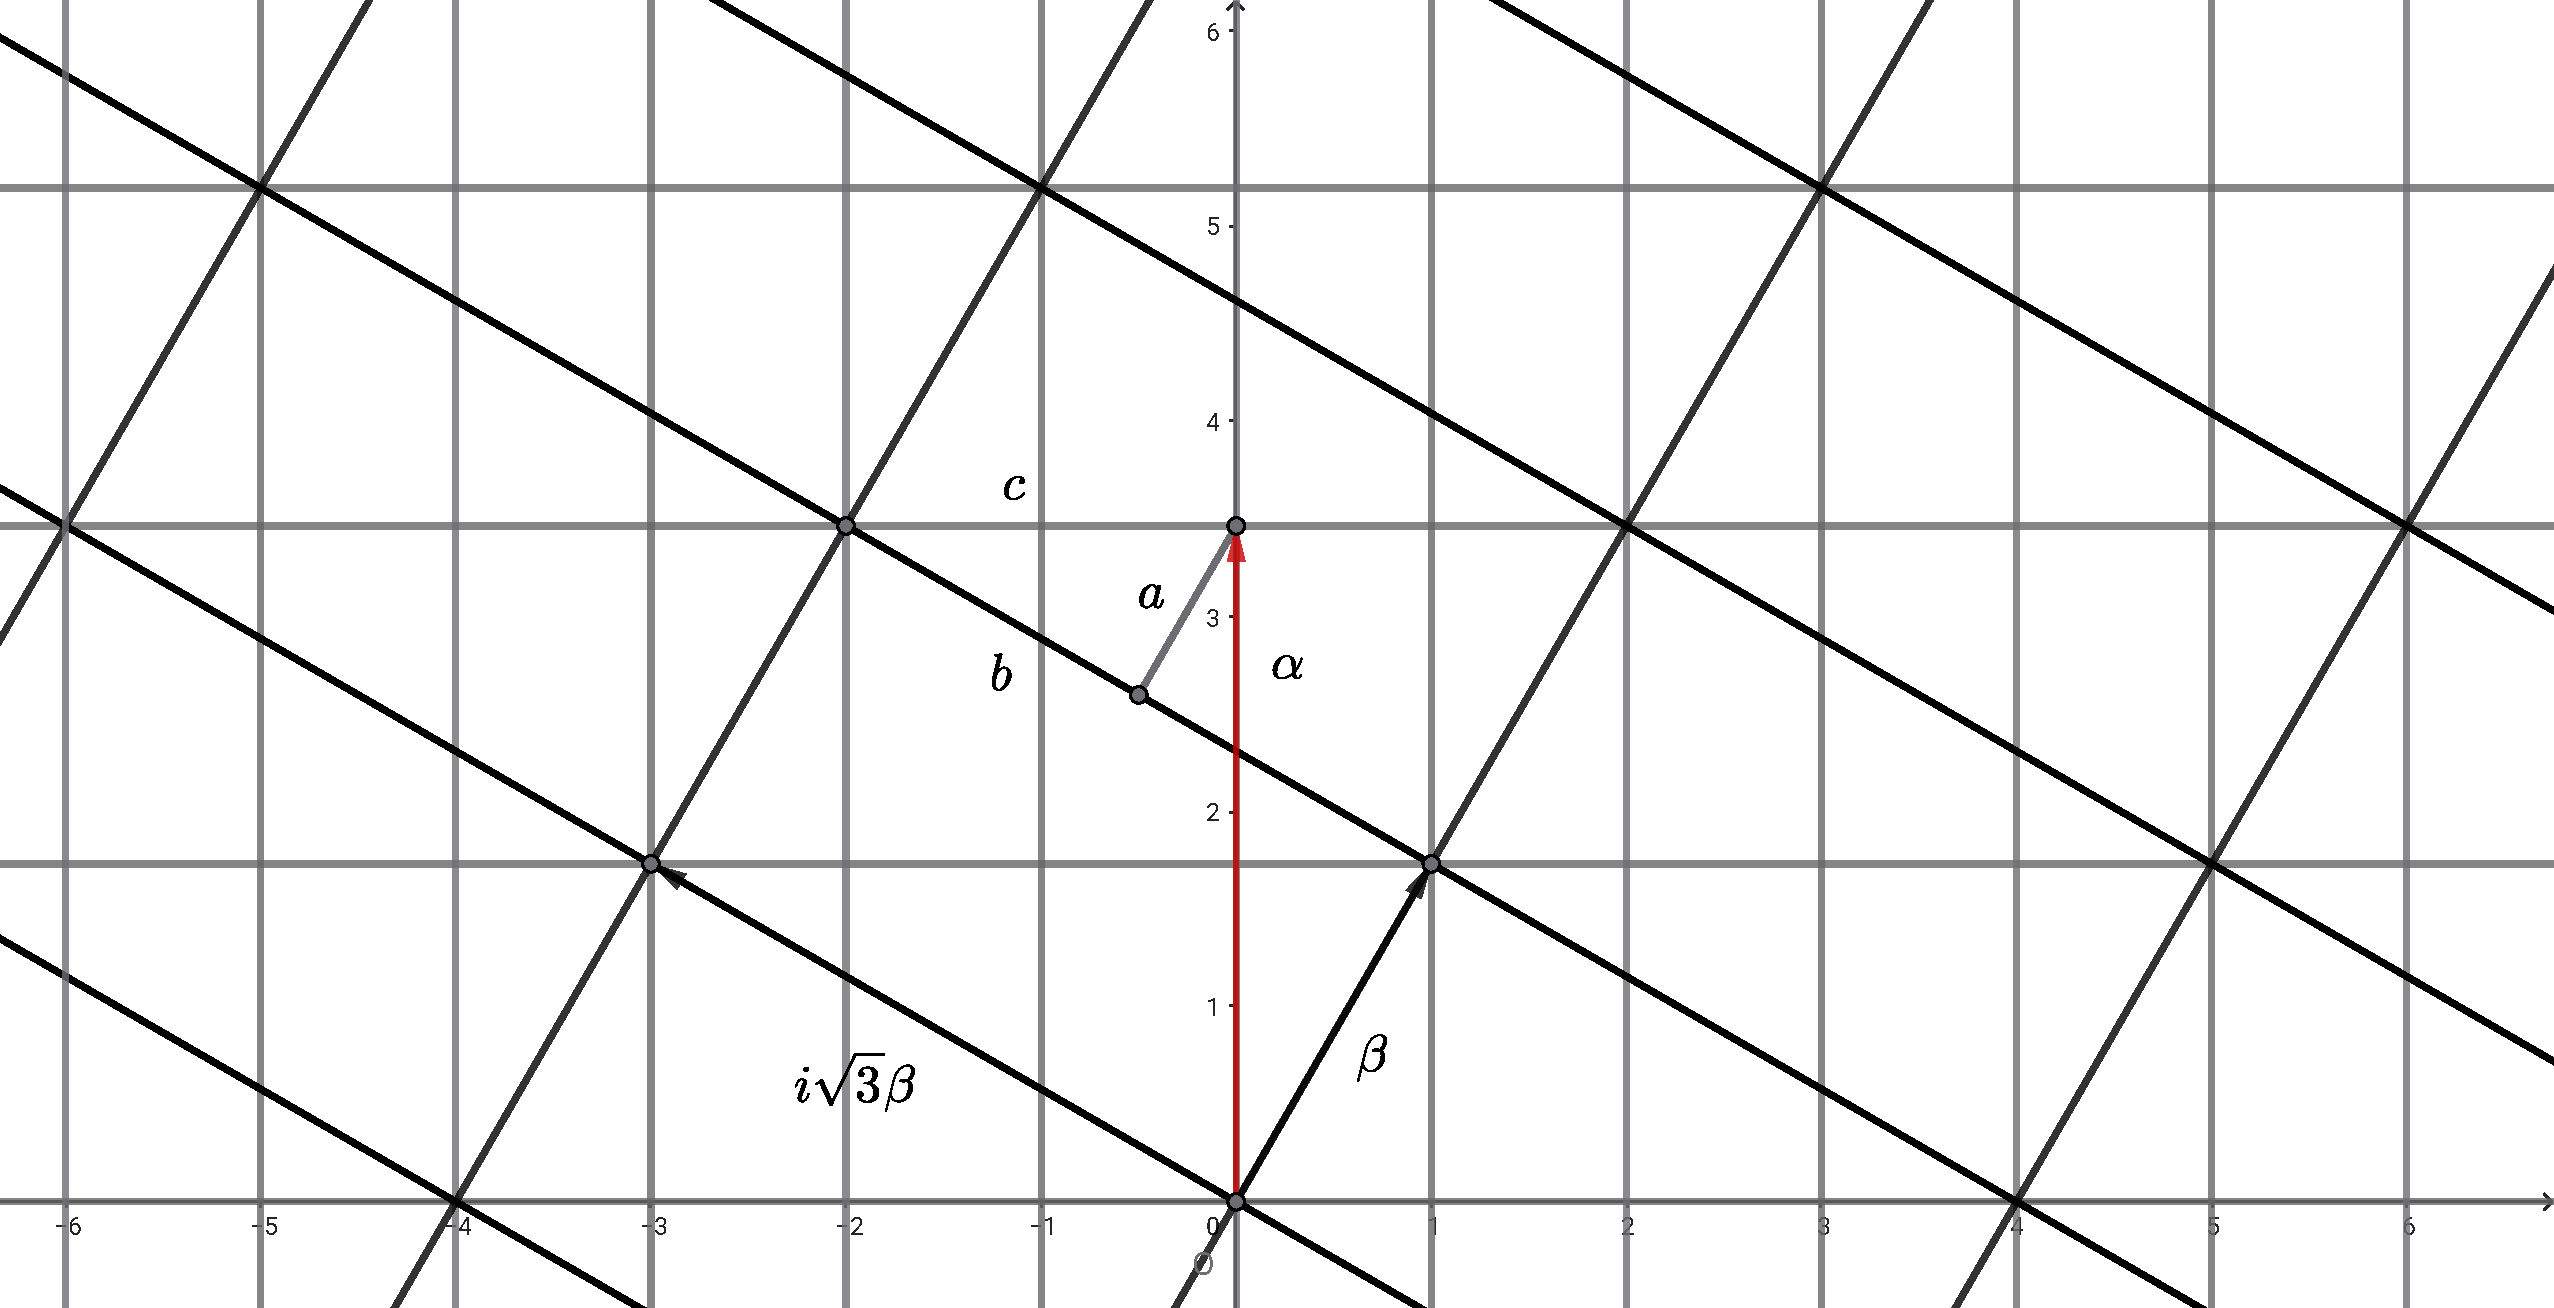
\includegraphics[scale=0.3]{img/z-sqrt-3}
 \caption{$\mathbb{Z}[\sqrt{-3}]$中的整数构成浅灰色网格,积$\rho \beta$构成黑色网格,$\alpha$落在某个格子中。}
 \label{fig:Z-sqrt-3}
\end{figure}

并不一定是$<$。如图中所示,当$\alpha$落在矩形中心时,不存在$\gamma$使得$N(\gamma) < N(\beta)$。因此欧几里得算法在$\mathbb{Z}[\sqrt{-3}]$上不成立,算术基本定理了不成立,分解不一定唯一。这就解释了$4 = 2 \times 2 = (1 + i\sqrt{3})(1 - i\sqrt{3})$。这真是太遗憾了!如果$\alpha$落在矩形中心以外的任何地方都能保证它到最近顶点的距离严格$< |\beta|$,只有中心是个例外。有没有办法补救呢?如\cref{fig:Z-omega}所示,这种情况下矩形的中心$\notin \mathbb{Z}[\sqrt{-3}]$。因而对所有的$\alpha$,都存在$\gamma$使得$N(\gamma) < N(\alpha)$。这两种情况有什么区别呢?似乎不同的$\beta$导致不同的结果。

\begin{figure}[htbp]
 \centering
 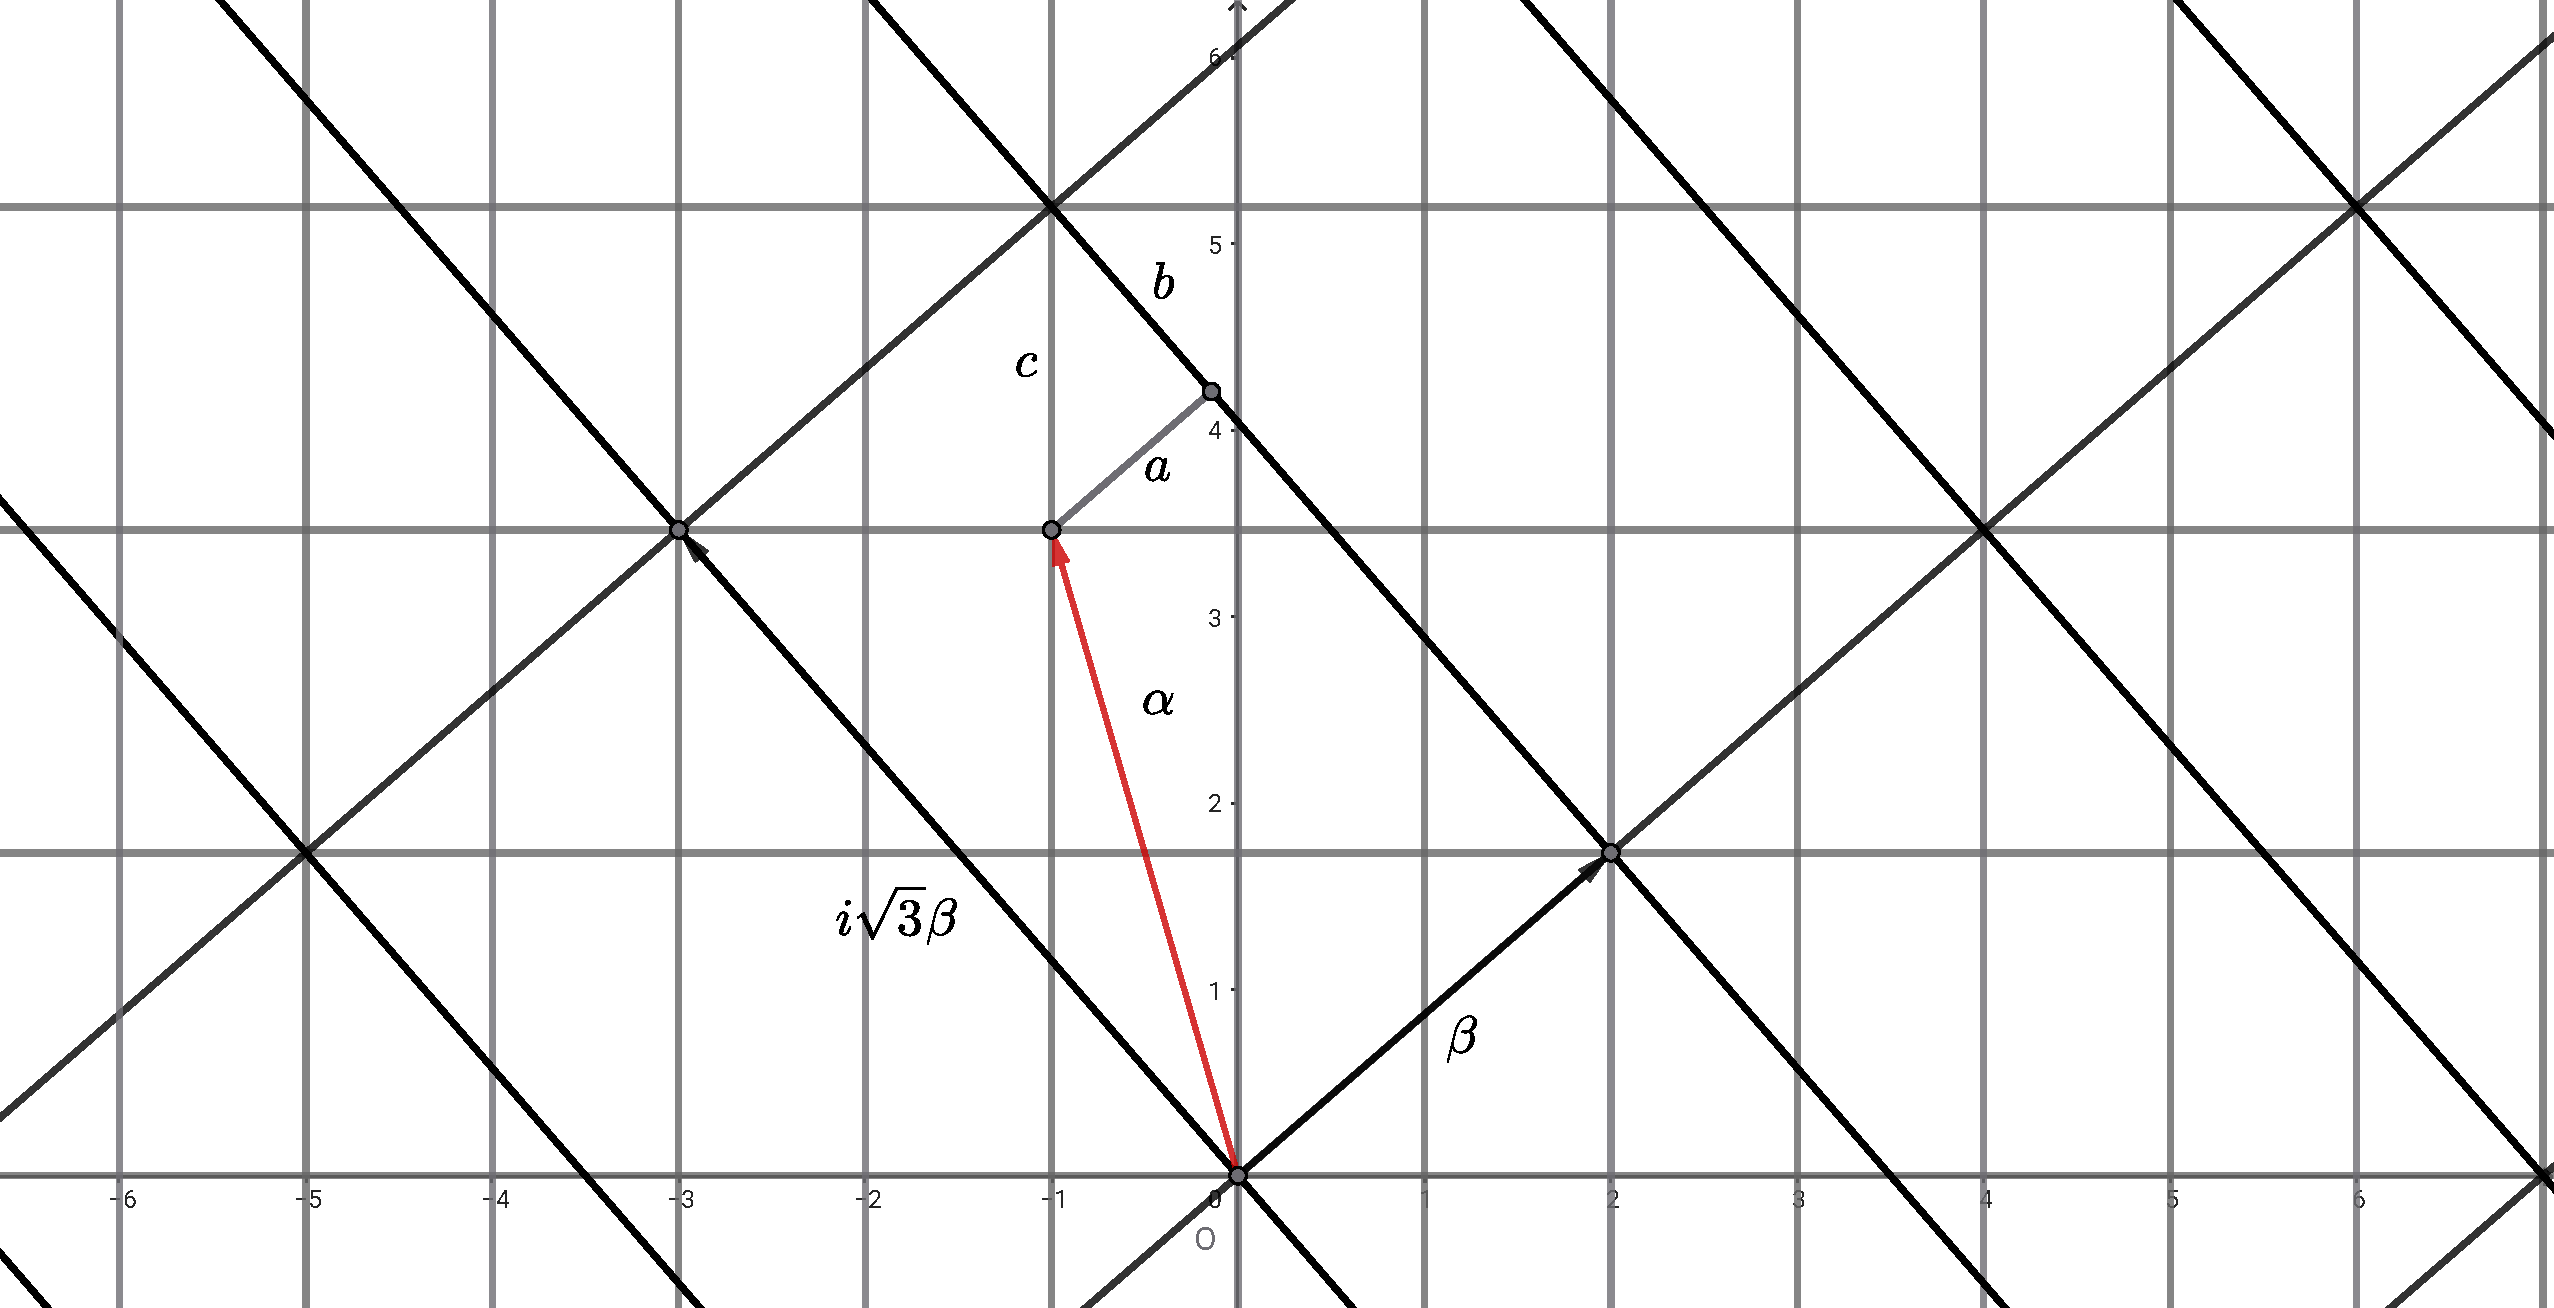
\includegraphics[scale=0.3]{img/z-omega}
 \caption{当$\beta = 2 + \sqrt{3}i$时,任何$\alpha$都不会落在$\rho \beta$网格的中心。此时可以找到$\gamma$使得$N(\gamma) < N(\beta)$。}
 \label{fig:Z-omega}
\end{figure}

让我们来分析一下,什么情况下矩形的中心不是二次整数。如\cref{fig:Z-sqrt-3c}所示,考虑任意$\rho \beta$构成的矩形,左下角$A$对应向量$\rho \beta$,根据复数加法的几何意义,右下角$C$对应向量$\rho \beta + \beta$,左上角$C'$对应$\rho \beta + i\sqrt{3}\beta$,即把向量$\beta$旋转90度后放大$\sqrt{3}$倍,再加到$C$上。矩形的中心就是对角线$CC'$的中心,对应向量:

\[
\frac{C + C'}{2} = \frac{\rho \beta + \beta + \rho \beta + i\sqrt{3}\beta}{2} = \rho \beta + \frac{1}{2}\beta + \frac{\sqrt{3}}{2}i\beta
\]

\begin{figure}[htbp]
 \centering
 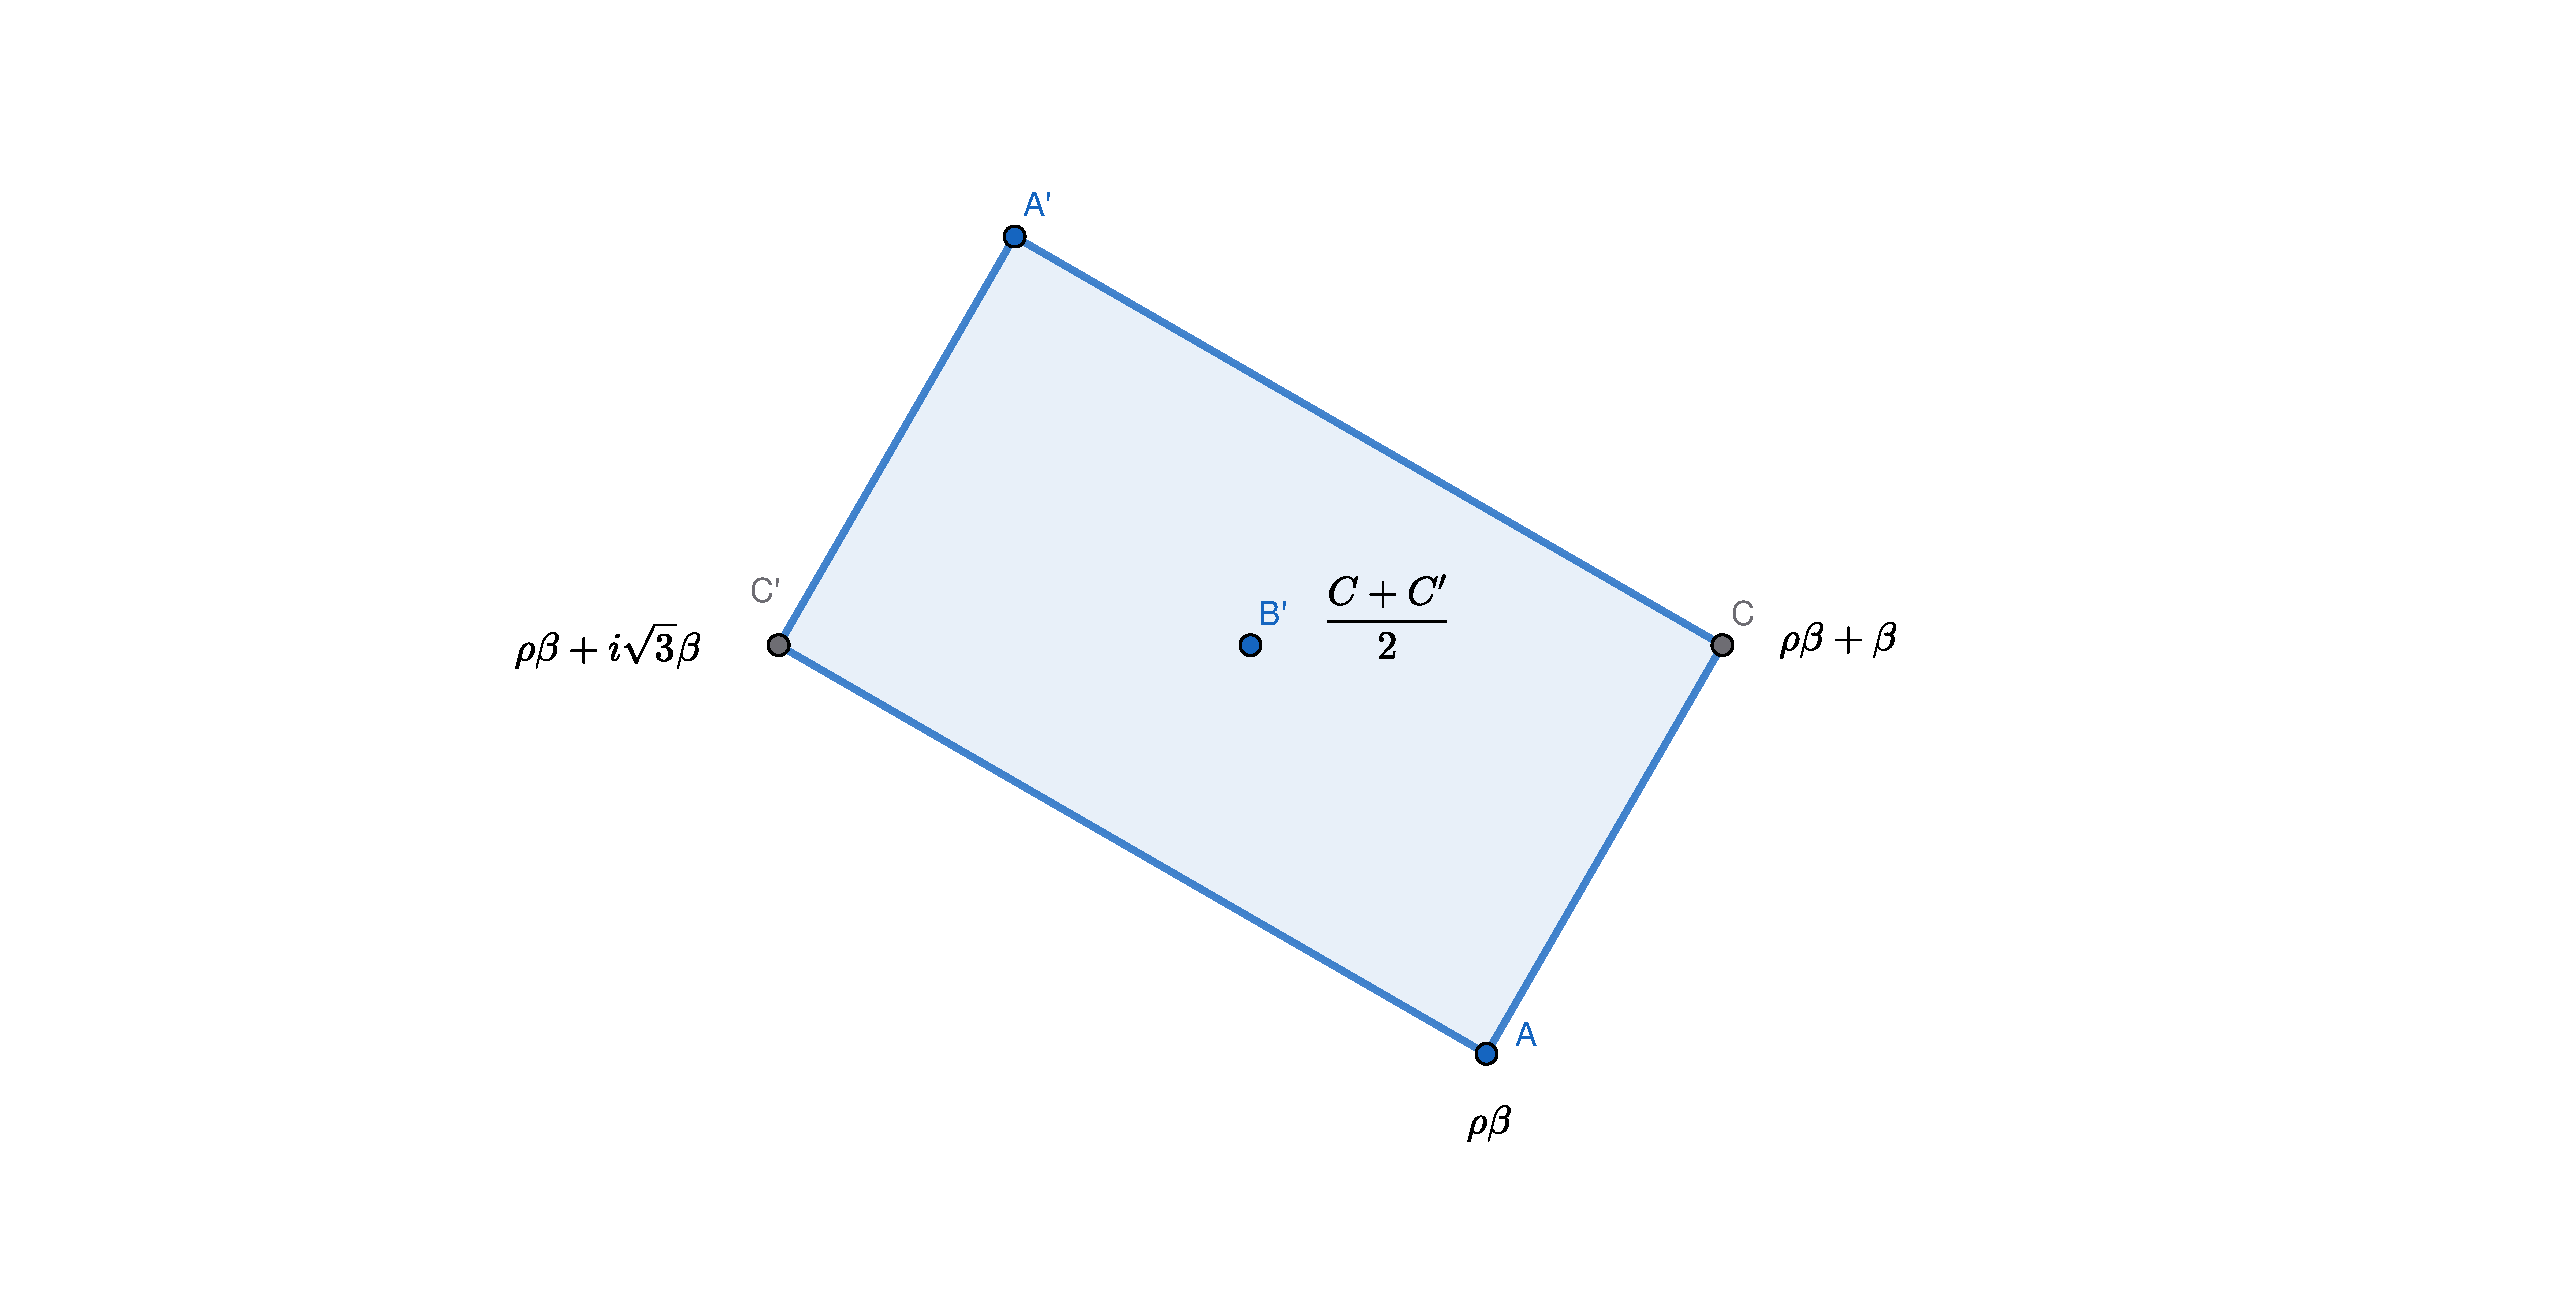
\includegraphics[scale=0.3]{img/z-sqrt-3c}
 \caption{$\rho \beta$组成的某个矩形及其中心。}
 \label{fig:Z-sqrt-3c}
\end{figure}

由于$\rho \beta \in \mathbb{Z}[\sqrt{-3}]$,所以当$\dfrac{1}{2}\beta + \dfrac{\sqrt{3}}{2}i\beta \notin \mathbb{Z}[\sqrt{-3}]$时,矩形的中心不是二次整数。令$\beta = a + bi\sqrt{3}$带入:

\[
\frac{a + bi\sqrt{3}}{2} + \frac{(a + bi\sqrt{3})i\sqrt{3}}{2} = \frac{a - 3b}{2} + \frac{a + b}{2}i\sqrt{3}
\]

如果$a-3b$或$a + b$是奇数,则矩形中心不是二次整数,此时必有$a, b$的奇偶不同。反之,如果$a, b$奇偶相同,矩形中心就是二次整数,欧几里得算法就会失效。在反例$4 = 2 \times 2 = (1 + i\sqrt{3})(1 - i\sqrt{3})$中,$a = b = 1$都是奇数。而在\cref{fig:Z-omega}中,$\beta = 2 + i\sqrt{3}$,其中$a = 2, b=1$奇偶不同,$\alpha$不可能是矩形中心,因此存在欧几里得算法,存在唯一分解。欧拉在证明费马大定理$n=3$时,的的确确要求$a, b$奇偶不同,这样就保证了唯一分解。所以当$a^2 + 3b^2$是立方数时,互素的$(a + bi\sqrt{3})(a - bi\sqrt{3})$每个都是立方数(\cref{qn:coprime-of-conjugates}要求证明$a \pm bi\sqrt{3}$互素)。

\index{爱森斯坦整数}
这样我们就给费马大定理$n=3$划上了句号。关于$\mathbb{Z}[\sqrt{-3}]$还有后继的故事。高斯整数是分布在正方形格子上的复数,爱森斯坦在1844年研究了分布在正三角形格子上的复数。今天我们把这样的复数叫做爱森斯坦整数。爱森斯坦发现很简单的首一二次方程$x^2 + x + 1 = 0$有两个解$\omega = \dfrac{-1}{2} \pm \dfrac{i\sqrt{3}}{2}$。根据代数整数的定义,尽管带有$\dfrac{1}{2}$,它们都是代数整数!更一般地,首一二次代数方程$x^2 - (2a - b)x + (a^2 - ab + b^2)$的解为$a + b \omega$。他们构成了爱森斯坦整数$\mathbb{Z}[\omega]$。爱森斯坦进一步定义范数为$N(a + b\omega) = a^2 -ab + b^2$(见\cref{qn:norm-of-z-omega}),并证明了欧几里得算法在$\mathbb{Z}[\omega]$上存在,从而唯一分解定理成立。而$\mathbb{Z}[\sqrt{-3}]$只不过是$\mathbb{Z}[\omega]$的一个子集。

\begin{mdframed}
爱森斯坦简介
\end{mdframed}

算术基本定理在高斯整数、$\mathbb{Z}[\sqrt{-2}]$、$\mathbb{Z}[\omega]$上成立是幸运的。一半来说它是不成立的。例如$\mathbb{Z}[\sqrt{-5}]$上的反例$6 = 2 \times 3 = (1 + i\sqrt{5})(1 - i\sqrt{5})$。我们可以证明$2, 3, 1 \pm i\sqrt{5}$都是不可分的。否则假设2可以分解为$(a + bi\sqrt{5})(c + di\sqrt{5})$,两边取范数:

\[
4 = N(2) = N(a + bi\sqrt{5})N(c + di\sqrt{5}) = (a^2 + 5b^2)(c^2 + 5d^2)
\]

首先可以排除$a^2 + 5b^2 = c^2 + 5d^2 = 2$的情况,因为此时$a, b, c, d$没有整数解。只能是$a^2 + 5b^2 = 1$或$c^2 + 5d^2 = 1$。范数为1对应单位元,另一个和2相伴。因此2不可分解。同样可证3不可分解。\cref{qn:1-n-delta-irreducible}要求用同样的方法证明$1 \pm i\sqrt{5}$不可分解。因此$6 = 2 \times 3 = (1 + i\sqrt{5})(1 - i\sqrt{5})$的确有两种分解方式。库默尔为此引入了理想数来挽救唯一分解,这在戴德金手中发展成了抽象武器——理想。

\section{理想}

这是北京市东城区高中一年级数学第一课《集合》的一道习题。

\begin{mdframed}
若非空数集$I, P$满足:

\begin{enumerate}[(i)]
\item 对任意的$x \in I$,有$x \in P$;
\item 对任意的$x, y \in I$,有$x + y \in I$;
\item 对任意的$x \in I$且对任意的$y \in P$,有$xy \in I$;
\end{enumerate}

则称$I$是$P$的“理想子集”。给出下列四个结论:

\begin{enumerate}[(a)]
%%   \renewcommand{\labelenumi}{\textcircled{\theenumi}}
\item 若$I = \{2k | k \in \mathbb{Z} \}$,则$I$是$\mathbb{Z}$的“理想子集”;
\item 若$I$是$\mathbb{R}$的“理想子集”,且存在非零实数$a \in I$,则$I = \mathbb{R}$;
\item 若$I_1, I_2$是$P$的“理想子集”,则$I_1 \cup I_2$也是$P$的“理想子集”;
\item 若$I_1, I_2$是$P$的“理想子集”,则$I_1 \cap I_2$也是$P$的“理想子集”。
\end{enumerate}

其中正确结论的序号是$\underline{\qquad \qquad}$

\end{mdframed}

这道题目只用最基本的集合论知识就能解答。其中第(i)条性质说$I$是$P$的子集;第(ii)条性质说$I$中的加法是封闭的,即$I$中的任何两个数的和还在$I$中;第(iii)条最抽象,它说用$P$中的任何$y$去缩放$I$中的任何$x$,结果$xy$还在$I$中。形象地说就是$I$对于缩放$P$封闭。我们接下来看4个选项。选项(a)中的$I$是全体偶数,任何偶数都是整数,所以(i)成立;偶数加偶数还是偶数,所以(ii)成立;偶数乘以任何整数还是偶数,所以(iii)成立。这样偶数的确是整数的“理想子集”,(a)正确。选项(b)抽象不好理解。这里的关键问题是1是否在$I$中?因为$a \ne 0$,所以倒数$\dfrac{1}{a} \in \mathbb{R}$存在。现在$a \in I, \dfrac{1}{a} \in \mathbb{R}$,根据性质(iii),$a\dfrac{1}{a} = 1 \in I$。一旦1在$I$中,任何实数$x \in \mathbb{R}$根据性质(iii)都有$1 \cdot x = x \in I$。因此$\mathbb{R}$就是$I$的子集,但性质(i)又说$I$是$\mathbb{R}$的子集,所以只能是$I = \mathbb{R}$,(b)正确。我们不妨用具体的例子来判断选项(c),仿照(a)中偶数的例子,令$I_1 = \{2k | k \in \mathbb{Z} \}, I_2 = \{5k | k \in \mathbb{Z} \}$,不难验证$I_2$,也就是5的倍数也是“理想子集”。它们的并集包含偶数或5的倍数,即$\{ \dotsc, 0, 2, 4, 5, 6, \dotsc\}$。我们立即发现$2 + 5 = 7$不在这个集合中。加法不封闭了,这违反了性质(ii),(c)错误。选项(d)把并集换成了交集。用同样的例子,$I_1$是偶数$I_2$是5的倍数,交集包含所有偶的5的倍数,即$\{\dotsc, -10, 0, 10, 20, \dotsc\}$。不难验证它是理想子集。但光验证还不够,我们需要严格证明它是对的。

\begin{proof}
任何$x \in I_1 \cap I_2$有$x \in I_1 \subseteq P$,所以(i)满足。任何$x, y \in I_1 \cap I_2$有$x, y \in I_1$,因$I_1$是“理想子集”,所以$x + y \in I_1$。另一方面也有$x, y \in I_2$,因$I_2$也是“理想子集”,所以$x + y \in I_2$。这样$x + y$既在$I_1$中也在$I_2$中,所以$x + y \in I_1 \cap I_2$。这样就证明了$I_1 \cap I_2$对加法封闭,满足(ii)。最后,任何$x \in I_1 \cap I_2, y \in P$有$x \in I_1$,因$I_1$是“理想子集”,所以$xy \in I_1$。另一方面也有$x \in I_2$,因$I_2$也是“理想子集”,所以$xy \in I_2$。这样$xy$既在$I_1$中也在$I_2$中,所以$xy \in I_1 \cap I_2$。这样就证明了性质(iii)。综上$I_1 \cap I_2$是“理想子集”。
\end{proof}

最后正确结论的序号是:$\underline{(a), (b), (d)}$。

这道题目意义非凡。它正是戴德金对理想的定义!唯一的额外要求是戴德金需要父集合$P$是一个“环”(ring),简单来说,就是定义了加法和乘法的集合\footnote{具体来说,要求满足加法、乘法的结合律、交换律,分配律,包含0和1。普通整数、高斯整数、二次整数都是环。}。我们以后用英文字母$R$来表示这个父集合。面对不唯一的分解$6 = 2 \times 3 = (1 + i\sqrt{5})(1 - i\sqrt{5})$,库默尔提出存在一种“理想数”,能够继续对$2, 3, 1 \pm i\sqrt{5}$分解。并且最终理想数的分解是唯一的。但究竟什么是理想数?戴德金的回答令人吃惊,理想(ideal)不再是具体的一个数,而是数的集合,并且是无穷集合!比如上面例子中的所有偶数,它们都是2的倍数,记为$(2)$,所有5的倍数记为$(5)$。如果一个理想$I$是某个$a$的倍数的集合,就叫做\underdot{主理想}(principle ideal),记作$(a)$。这和我们此前定义数的方式大相径庭。历史上第一个用集合来定义数的人是逻辑学家弗雷格。我们知道数具有抽象的含义。3可以代表3个人、三个鸡蛋、图形中的三角等等,这些类\footnote{弗雷格的工作在康托尔之前,他当时使用了“类”(class)一词。康托尔后来使用了德语中的“集合”。}都有三个元素,用哪一个来代表自然数3呢?弗雷格的意见是:全部。即所有能和上述类一一对应的类所组成的、无穷的、抽象的类来定义自然数3。弗雷格的这一定义看起来有些复杂,但是很了不起。它突破了文化背景的限制。不管你是使用何种语言,何种符号,按照弗雷格的方法,对数字3的理解都不会有歧义。

\begin{figure}[htbp]
 \centering
 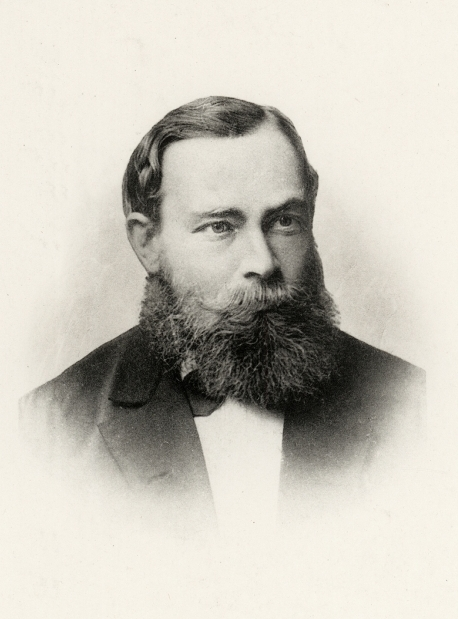
\includegraphics[scale=0.9]{img/Frege}
 \caption{戈特洛布·弗雷格(1848-1925)}
 \label{fig:Frege}
\end{figure}

理想究竟是怎样挽救唯一分解的呢?戴德金首先使用理想的语言重新定义了除法和最大公约数等概念。在普通整数中,我们说2整除6,3整除6,2和3的最大公约数是$(2, 3) = 1$。我们看一看理想$(2), (3), (6)$的关系:(2)包括所有偶数,(6)包括所有6的倍数,偶数包含所有6的倍数,即(2)包含(6);理想(3)包含所有3的倍数,自然也包含所有6的倍数,所以(3)包含(6)。

\btab{c||c}
2整除6 & 3整除6 \\
(2)包含(6) & (3)包含(6)
\etab

这样理想间的包含就对应着整数间的整除,用一句话概括就是\underdot{整除即包含}。我们可以证明这一结论:

\begin{proposition}
如果$a$整除$b$,则理想$(a)$包含理想$(b)$。
\end{proposition}

\begin{proof}
由整除的定义,存在$c$使得$ac = b$。任何$x \in (b)$可表示为:
\begin{align*}
x &= bk  &&\text{其中}k \in R \\
  &= ack &&\text{整除的定义} \\
  &= ak' \in (a) &&\text{令}k' = ck \in R \qedhere
\end{align*}
\end{proof}

接下来考虑最大公约数。定义理想间的加法为:$I_1 + I_2 = \{a + b | a \in I_1, b \in I_2\}$(\ref{qn:sum-of-ideals}要求证明理想的和仍是理想)。这样在上面的例子中,理想的和为:

\[
(2) + (3) = \{a + b| a \in (2), b \in (3)\} = \{2x + 3y | x, y \in \mathbb{Z} \}
\]

这是由2和3产生出来的数构成的集合,我们也用符号$(2, 3)$表示理想的和。你也许联想到了最大公约数的符号。如果2和3的最大公约数是$d = (2, 3) = 1$,根据定义$d$整除2也整除3,所以$d$整除任何$2x + 3y$。这样理想的和就是$(d)$,也就是(1)。

\[
(2) + (3) = \{2x + 3y\} = \{dk | k \in \mathbb{Z}\} = (d) = (1)
\]

我们把这条结论归纳如下。
\begin{proposition}
如果$a, b$的最大公约数为$d = (a, b)$,则$(a) + (b) = (d)$。
\end{proposition}

\begin{proof}
根据定义:
\begin{align*}
(a) + (b) &= \{ax + by | x, y \in R\} \\
  &= \{dmx + dny | m, n, x, y \in R\} && d\text{是最大公约数,令}a = dm, b = dn \\
  &= \{d(mx + ny) | m, n, x, y \in R\} && \text{令}k = mx + ny \\
  &= \{dk | k \in R \} = (d) && \qedhere
\end{align*}
\end{proof}

显然任何整数$a$都可生成主理想$(a)$,也就是$a$的倍数的集合(\cref{qn:trivial-ideals}要求思考(0)和(1))。但整数中的任何理想都是主理想么?这个问题相当于任何理想都等价于某个整数$a$的倍数集合么?

\begin{proposition}
整数中的任何理想都是主理想。
\end{proposition}

\begin{proof}
对整数中的任何理想$I$,找出其中绝对值最小的非零元素$b$。整数绝对值的性质保证了若$I \ne (0)$则$b$存在。我们声称$I = (b)$。否则若存在某个元素$a \in I$,但$a \notin (b)$,由欧几里得算法$r = a - bq$,并且$|r| < |b|$。根据理想的定义$a \in I, bq \in I$,所以$r = a - bq \in I$。但$r$的绝对值小于$b$的绝对值,由于我们选择的$b$是绝对值\underdot{最小}的非零元素,因此只能有$r = 0$,即$b$整除$a$。
\end{proof}

我们看到绝对值和存在欧几里得算法在证明中的关键作用。用类似的办法,我们也可以证明高斯整数中的任何理想都是主理想。

\begin{proposition}
高斯整数中的任何理想都是主理想。
\end{proposition}

\begin{proof}
对高斯整数中的任何理想$I$,找出其中范数最小的非零元素$\beta$。高斯整数范数的性质保证了若$I \ne (0)$则$\beta$存在。我们声称$I = (\beta)$。否则若存在某个元素$\alpha \in I$,但$a \notin (\beta)$,由欧几里得算法$\gamma = \alpha - \beta \rho$,并且范数$N(\gamma) < N(\beta)$。根据理想的定义$\alpha \in I, \beta \rho \in I$,所以$\gamma = \alpha - \beta \rho \in I$。但$\gamma$的范数小于$\beta$的范数,由于我们选择的$\beta$是范数\underdot{最小}的非零元,因此只能有$\gamma = 0$,即$\beta$整除$\alpha$。
\end{proof}

这个结论还有对应的几何意义。任何高斯整数$\beta$的倍数$\rho \beta$是边长为$|\beta|$正方形网格。而$\beta$的倍数恰恰是理想$(\beta)$。特别地,理想$(1)$是边长为1的正方形网格。高斯整数中所有理想对应的网格都是正方形,都和(1)相似,如\cref{fig:zi}所示。同样的结论对$\mathbb{Z}[\sqrt{-2}]$也成立。任何$\beta$的倍数都是长$\sqrt{2}|\beta|$宽$|\beta|$的矩形。$\mathbb{Z}[\sqrt{-2}]$中所有理想都是主理想,都对应着相似的矩形网格(长宽比为$\sqrt{2}$,如\cref{fig:Z-sqrt-2}所示)。

但$\mathbb{Z}[\sqrt{-5}]$就不同了,它包含着不相似的网格。唯一分解在$\mathbb{Z}[\sqrt{-5}]$上失效,存在反例$6 = 2 \times 3 = (1 + i\sqrt{5})(1 - i\sqrt{5})$。我们考虑理想的和:

\begin{align*}
A &= (2) + (1 + i\sqrt{5}) = \{2\alpha + (1 + i\sqrt{5})\beta | \alpha, \beta \in \mathbb{Z}[\sqrt{-5}]\} \\
  &= \{2(a + bi\sqrt{5}) + (1 + i\sqrt{5})(c + di\sqrt{5}) | a, b, c, d \in \mathbb{Z}\} \\
  &= \{(2a + c - 5d) + (2b + c + d)i\sqrt{5} | a, b, c, d \in \mathbb{Z} \} \\
  &= \{2(a - b - 3d) + (2b + c + d)(1 + i\sqrt{5}) | a, b, c, d \in \mathbb{Z} \} \\
  &= \{2m + (1 + i\sqrt{5})n | m, n \in \mathbb{Z} \} \\
  &= (2, 1 + i\sqrt{5}) && \text{由}2, 1+ i\sqrt{5}\text{产生的数}
\end{align*}

\begin{figure}[htbp]
 \centering
 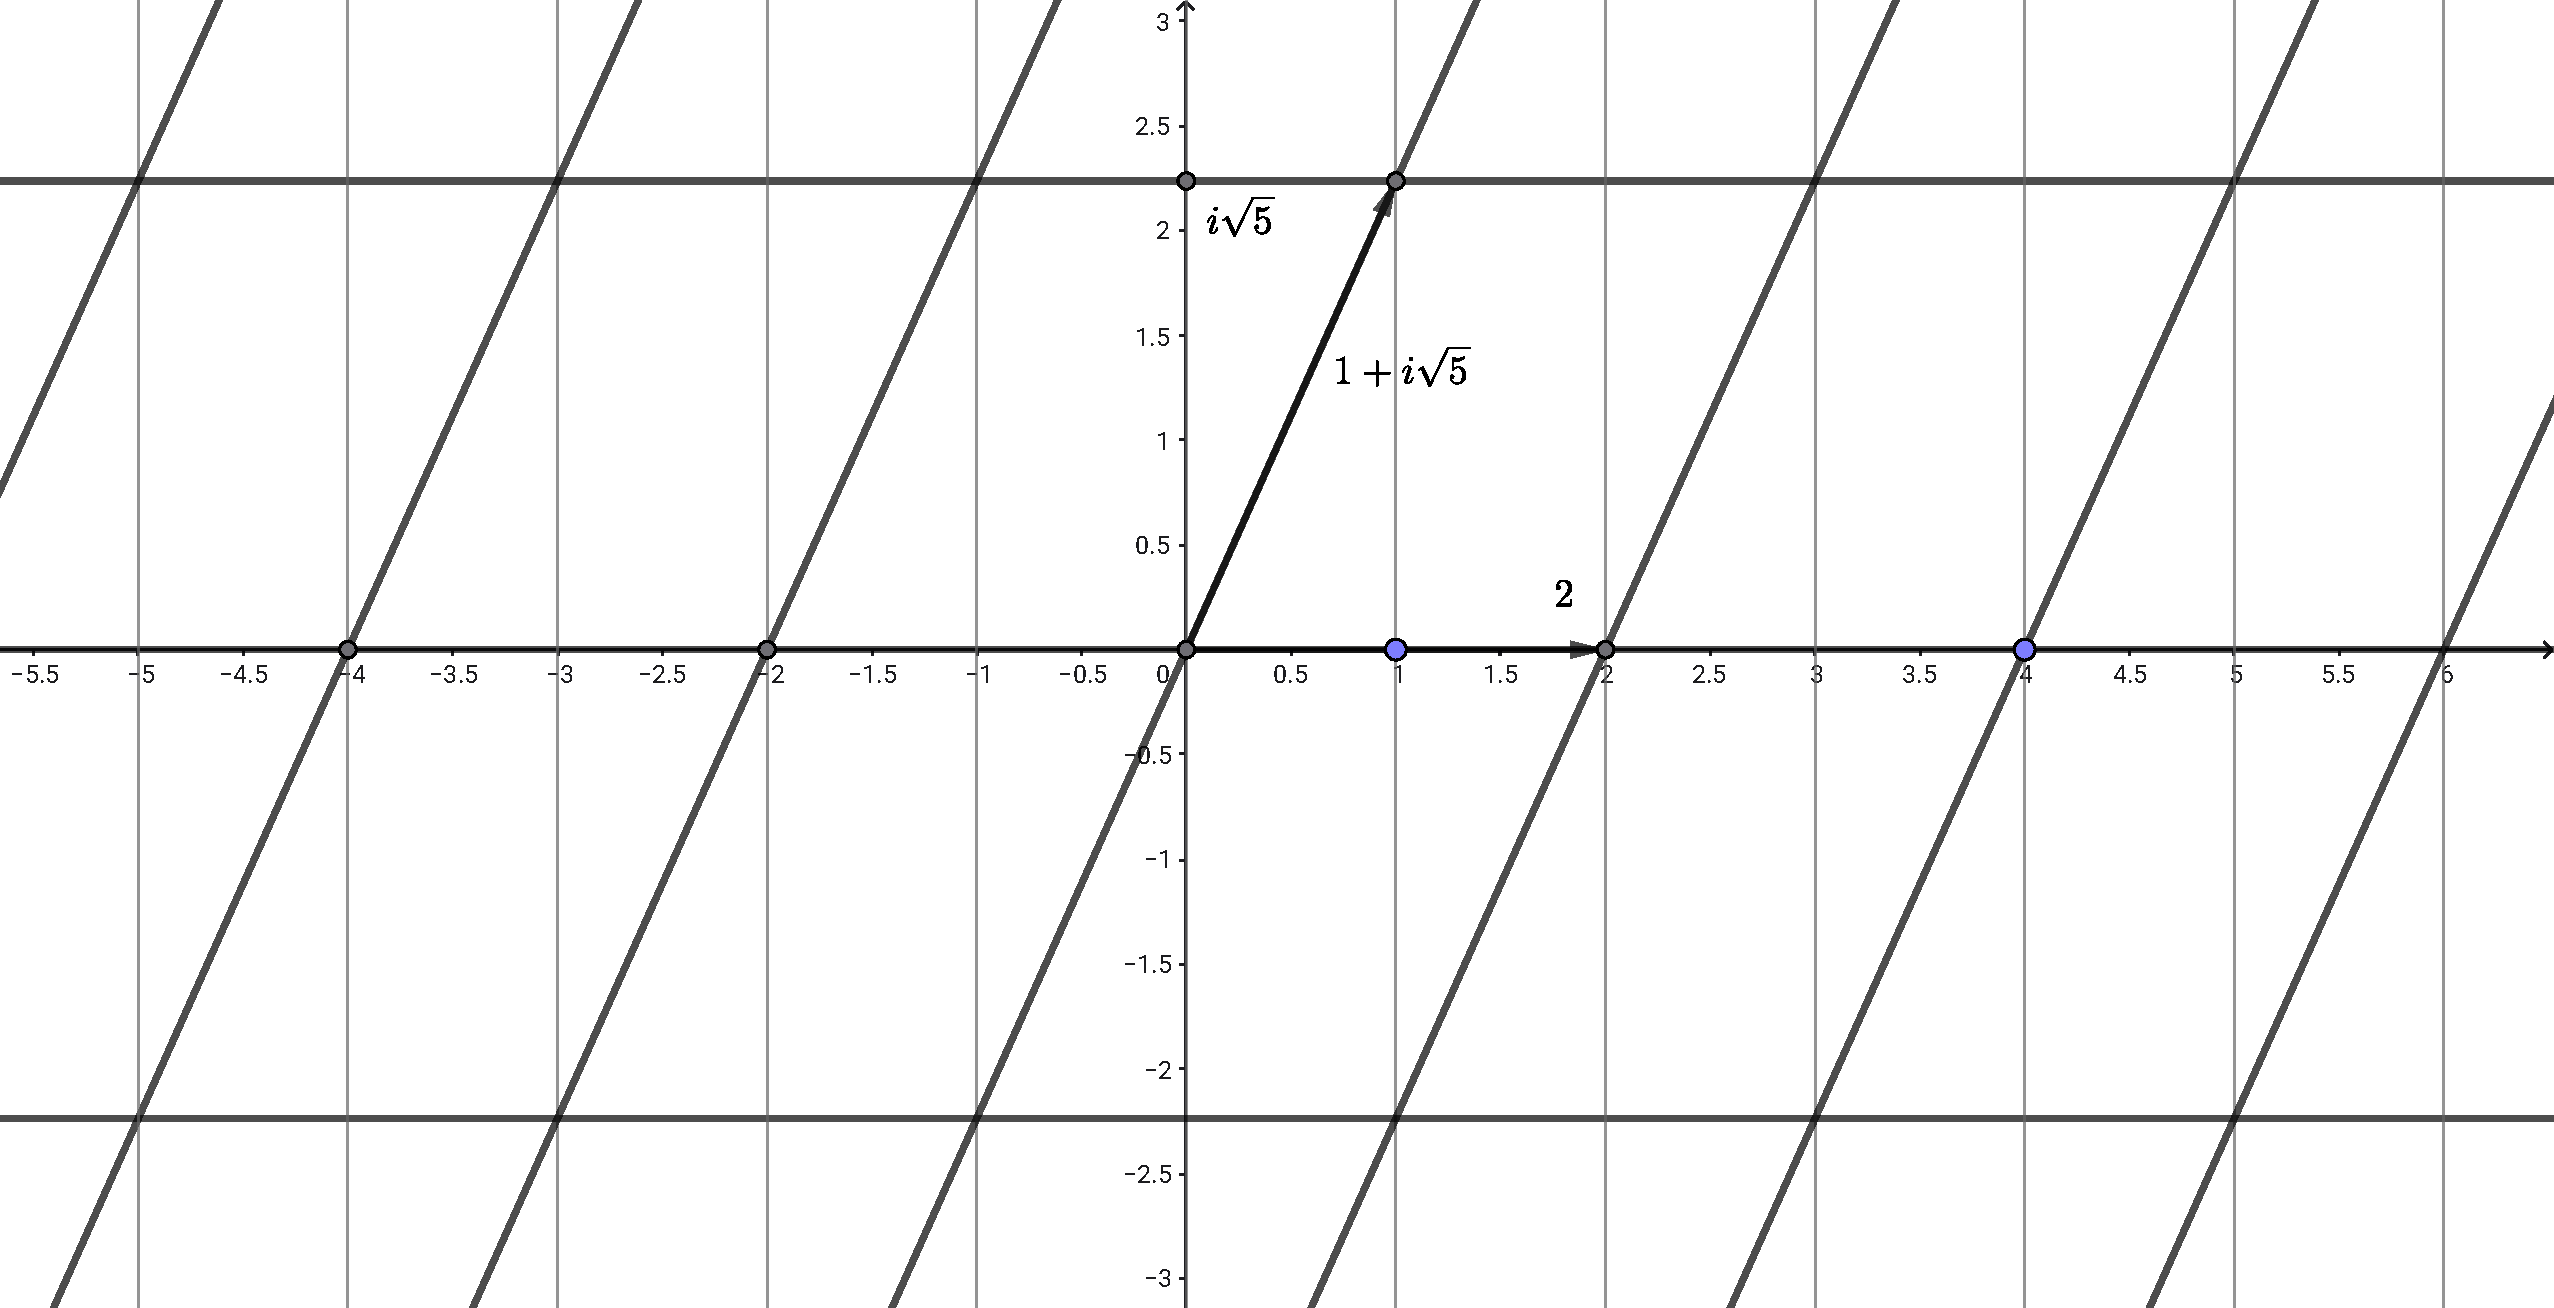
\includegraphics[scale=0.3]{img/ideal-sum}
 \caption{灰色矩形网格为$\mathbb{Z}{\sqrt{-5}}$中的整数,黑色三角形网格为$(2, 1 + i\sqrt{5})$。}
 \label{fig:ideal-sum}
\end{figure}

在整数和高斯整数中,任何理想都是主理想,所以理想的和也是主理想。但$A = (2, 1 + i\sqrt{5})$却不是主理想。否则假设它是$(\gamma)$,因为2在这个理想中,所以$\gamma$整除2。但我们之前分析过2是不可分解的,因此$\gamma$只能是单位元或2的相伴元。另一方面$1 + i\sqrt{5}$也在这个理想中,所以$\gamma$整除$1 + i\sqrt{5}$。但$1 + i\sqrt{5}$也不可分解(见\cref{qn:1-n-delta-irreducible}),因此$\gamma$只能是单位元或$1 + i\sqrt{5}$的相伴元。这样综合下来$\gamma$只能是单位元。但是$\pm 1$却不在$(2, 1 + i\sqrt{5})$中,否则假设:

\begin{align*}
\pm 1 &= 2m + (1 + i\sqrt{5})n &&m, n\text{是整数} \\
  &= 2m + n + ni\sqrt{5}
\end{align*}

由实部虚部分别相等有:

\begin{align*}
\pm 1 &= 2m + n & n = 0
\end{align*}

得$m = \pm\dfrac{1}{2}$,与$m$是整数矛盾。因此$A = (2, 1 + i\sqrt{5})$不是主理想。它的网格形状不是矩形而是三角形,如\cref{fig:ideal-sum}所示。尽管不是主理想,但是$A$表现得像“最大公约数”。根据“整除即包含”,$A$包含(2),它表现得像2的因子,同时$A$包含$(1 + i\sqrt{5})$,它也表现得像$1 + i\sqrt{5}$的因子,因此$A$表现得像2与$1 + i\sqrt{5}$的最大公因子(类比整数和高斯整数,若$a, b$的最大公约数为$d = (a, b)$,则$(a) + (b) = (d)$)。

不仅如此,$A$还表现得像素数。为此我们先观察一下普通素数$p$在整数中的主理想$(p)$有什么特点。首先$p \ne 1$。而(1)实际上是全体整数(见\cref{qn:trivial-ideals}),理想$(p)$的确不是全体整数,因为1不在其中。其次$p$只能被1和它自己整除,根据“整除即包含”,只有代表全体整数的(1)包含$(p)$,再没有其它理想包含$(p)$了。$A$也是如此,首先它不是(1),我们此前证明了$1 \notin A$。其次除了(1)外没有任何理想包含$A$,否则假设存在一个理想$I$包含$A$且$I$中还有不在$A$中的元素,形如$\alpha = 2m + 1 + n(1 + i\sqrt{5})$。但是$\alpha - 1 = 2m + n(1 + i\sqrt{5})$就属于$A$了。并且$1 - \alpha$也属于$A$。现在$\alpha \in I, 1 - \alpha \in A \subset I$,根据理想的定义$\alpha + (1 - alpha) = 1 \in I$。于是$I = (1)$。

用同样的方法,我们也可以证明$\overline{A} = (2, 1 - i\sqrt{5}$表现的像素数。我们特意选用了共轭复数的符号,因为$\overline{A}$中的数恰好是$A$中的共轭复数。我们还可以利用$6 = 2 \times 3 = (1 + i\sqrt{5})(1 - i\sqrt{5})$的这四个因子构造出四个类似的理想:

\begin{align*}
A &= (2, 1 - i\sqrt{5})  & \overline{A} &= (2, 1 - i\sqrt{5}) &
B &= (3, 1 - i\sqrt{5})  & \overline{B} &= (3, 1 - i\sqrt{5})
\end{align*}

戴德金在1871年定义了理想间的乘积。如果$A, B$是理想,则:

\[
AB = \{a_1b_1 + a_2b_2 + \dotsb + a_kb_k\}
\]

其中$a_1, a_2, \dotsc, a_k \in A, b_1, b_2, \dotsc, b_k \in B$是各自理想中的元素。这样如果理想$C = AB$,则理想$A$整除理想$C$。根据戴德金的这个定义,主理想的乘积也是主理想,即$(a)(b) = (ab)$。因此$(a)$整除$(ab)$。例如$(2)(3) = (6)$,理想$(2)$整除$(6)$与整数的整除对应。如果理想$A$由$(a, b)$产生,理想$B$由$(c, d)$产生,则$AB = (ac, ad, bc, bd)$(见\ref{qn:ideal-product})。我们接下来计算一下$A\overline{A}$的结果:

\[
A\overline{A} = (2, 1 + i\sqrt{5})(2, 1 - i\sqrt{5}) = (4, 2 + 2i\sqrt{5}, 2 - 2i\sqrt{5}, 6)
\]

其中$4, 6, 2 \pm 2i\sqrt{5}$都能被2整除。根据“整除即包含”,主理想$(2)$包含$A\overline{A}$。另一方面,$4 \in A\overline{A}, 6 \in A\overline{A}$,所以$6 - 4 = 2 \in A\overline{A}$。这样$(2)$又被$A\overline{A}$包含。因此只能是$A\overline{A} = (2)$。用同样的方法我们可以证明$B\overline{B} = (3)$。我们再计算乘积$AB$的结果:

\[
AB = (2, 1 + i\sqrt{5})(3, 1 + i\sqrt{5}) = (6, 2 + 2i\sqrt{5}, 3 + 3i\sqrt{5}, (1 + i\sqrt{5})^2)
\]

其中$6, 2 + 2i\sqrt{5}, 3 + 3i\sqrt{5}, (1 + i\sqrt{5})^2$每个都能被$(1 + i\sqrt{5})$整除。根据“整除即包含”,主理想$(1 + i\sqrt{5})$包含$AB$。另一方面,$2 + 2i\sqrt{5} \in AB, 3 + 3i\sqrt{5} \in AB$,所以差$2 + 2i\sqrt{5} \in AB$。这样$(1 + i\sqrt{5})$又被$AB$包含。因此只能是$AB = (1 + i\sqrt{5})$。用同样的方法我们可以证明$\overline{AB} = (1 - i\sqrt{5})$。把这些结果放到一起就得到:

\[
(6) = (2)(3) = (A\overline{A})(B\overline{B}) = (AB)(\overline{AB}) = (1 + i\sqrt{5})(1 - i\sqrt{5})
\]

这样戴德金就用理想挽救了唯一分解。$(6)$被唯一分解为$A\overline{A}B\overline{B}$。

\section{谁更多?}

\index{伽利略悖论}

\begin{figure}[htbp]
 \centering
   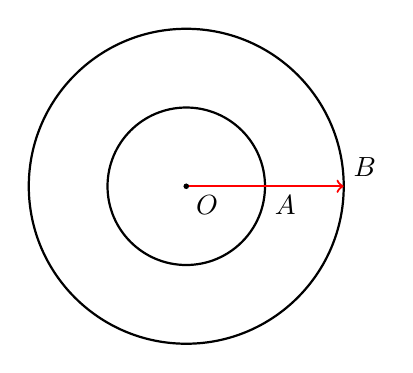
\begin{tikzpicture}[
       scale=0.5,
       circle_style/.style={draw, black, thick}, % 圆的样式:黑色、粗线条
       radius_style/.style={draw, red, thick, ->} % 半径的样式:红色、粗线条、带箭头
   ]

   % 1. 绘制内圆(圆心在坐标原点(0,0),半径2cm)
   \draw[circle_style] (0,0) circle (2cm);

   % 2. 绘制外圆(同一圆心(0,0),半径4cm,与内圆同心)
   \draw[circle_style] (0,0) circle (4cm);

   % 3. 绘制半径(从圆心(0,0)指向外圆上的点(4,0),沿x轴正方向)
   % 注:箭头指向外圆,因此终点坐标需与外圆半径匹配(x=4cm, y=0,即(4,0))
   \draw[radius_style] (0,0) -- (4,0);

   \fill[black] (0,0) circle (2pt);
   \node[below right] at (0,0) {$O$};
   \node[below right] at (2,0) {$A$};
   \node[above right] at (4,0) {$B$};

   \end{tikzpicture}

 \caption{同心大圆上任意一点都可通过半径对应到小圆上的唯一点}
 \label{fig:circles-paradox}
\end{figure}

我们数的旅程逐渐接近尾声。我们一路走来,探寻了自然数、零、整数、有理数、无理数、实数、复数、代数数。这些数有的彼此包含,例如自然数是整数的一部分;也有的是彼此独立,例如有理数和无理数。那么谁更多呢?在数的大家庭中,是否我们生活中常见的数更多,而罕见的数较少?也许生活会欺骗我们,也许直觉靠不住。这个问题的困难之处在于,除了零以外,每种数都有无穷多。无穷有多大?自然是要多大有多大,但这样一来怎样比较呢?举例来说,有人认为偶数只有整数的一半,所以整数更多。但是任何整数乘以2,就得到一个偶数,反之,任何偶数除以2,也对应一个整数。这样看来整数和偶数间一一对应,这两个集合似乎又同样多。究竟是整数多还是偶数多呢?现代科学之父伽利略在1636年提出一个类似的悖论。如果将每个自然数平方,得到的新序列$1, 4, 9, 16, 25, \dotsc$和自然数一一对应。这样看来完全平方数和自然数一样多。可是平方数很稀疏,自然数似乎比平方数多得多。这一矛盾被称为“伽利略悖论”。在几何上人们同样发现了类似的悖论。如\cref{fig:circles-paradox}所示,大圆似乎比小圆包含更多的点。但每条半径把两个同心圆上的点连接起来。大圆上任意一点都一一对应到小圆上的一点。这样看来两个圆上的点似乎同样多。伽利略发现无法解释自然数和平方数孰多孰少后说:因此我们不能说自然数构成一个集合。人们拒绝“全体自然数”这类说法。

两百年后,数学家康托尔重新思考了陷入矛盾的一系列悖论,问题的关键在于根深蒂固的常识——整体大于部分。并不适用于抽象的无限概念。康托尔认为,如果接受“部分能够等于整体”的观点,解决问题的大门就打开了。他提出了用一一对应来比较集合的大小的方法。康托尔定义:如果能够建立集合$A$和集合$B$中元素的一一对应关系,那么这两个集合具有相同的基数(cardinal number),或者说它们是“等势”的,记作$A \cong B$。对于有限集,这一结论显然正确;推广到无限集,根据此定义,偶数和整数同样多,完全平方数和自然数同样多,小圆和大圆上的点也同样多……戴德金干脆这样定义无穷集合:如果一个集合的部分和整体可以具有相同的基数,那么这个集合是无穷集合\cite{Dedekind-1858}。

乔治・伽莫夫1947年在科普著作《从一到无穷大》中讲了一个脍炙人口的故事。这则故事来自数学家希尔伯特在1924年冬季的一次演讲\footnote{希尔伯特的讲稿直到2013年才出版。}。有一个神奇的旅馆,拥有无穷多的房间。在旅游旺季的时候,旅馆住满了客人,已经满员了。这一天晚上,又来了一名客人。要是一般的旅馆,就只能拒绝这个新客人入住了。旅店经理希尔伯特说:“没问题,住得下。”他于是指挥客人,让1号房间的客人搬到2号房间去,2号房间的客人搬到3号房间去,3号房间的客人搬到4号房间去……每个房间的客人都搬到下一个房间去。这样就空出了1号房间给新来的这位客人。

故事没有结束。第二天,旅店迎来了一个神奇的旅游团,它有无穷多的游客。酒店经理希尔伯特又说:“没问题,住得下。”他指挥房间里的客人。让昨天住进1号房间的那位新客人搬到2号房间去,让2号房间的客人搬到4号房间去,让3号房间的客人搬到6号房间去……每个房间的客人都搬到房间号2倍的那个房间去。由于酒店有无穷多的房间,所以这样一搬,2, 4, 6, ...这些偶数房间住着原来的客人。而1, 3, 5, ...这些奇数房间空出来,有无穷多间。刚好可以让旅游团的人一人一间住下。故事更加有趣了。到了第三天,旅馆门前车水马龙,来了无穷多的神奇旅游团,每个旅游团都有无穷多位游客。希尔伯特的无穷旅馆还能住下么?

\begin{figure}[htbp]
 \centering
 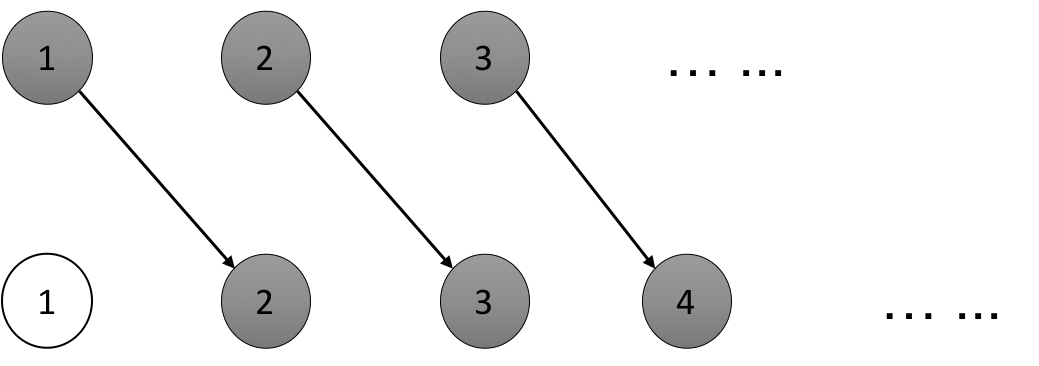
\includegraphics[scale=0.4]{img/Hilbert-hotel-1}
 \caption{希尔伯特无穷旅馆的第一天}
 \label{fig:Hilbert-hotel-1}
\end{figure}

如\cref{fig:Hilbert-hotel-1}所示,在第一天的故事中,每个客人搬到下一个房间去,从而空出1号房间。这建立了图中上下两行灰色圆形之间的一种对应关系$n \leftrightarrow n+1$。这告诉我们一个有趣的事实:无穷加上1还是无穷。不仅如此,即使来了有限多$k$位新客人,我们可以重复这一“腾笼换鸟”的过程$k$次,仍然能够让他们入住满员的宾馆。

\begin{figure}[htbp]
 \centering
 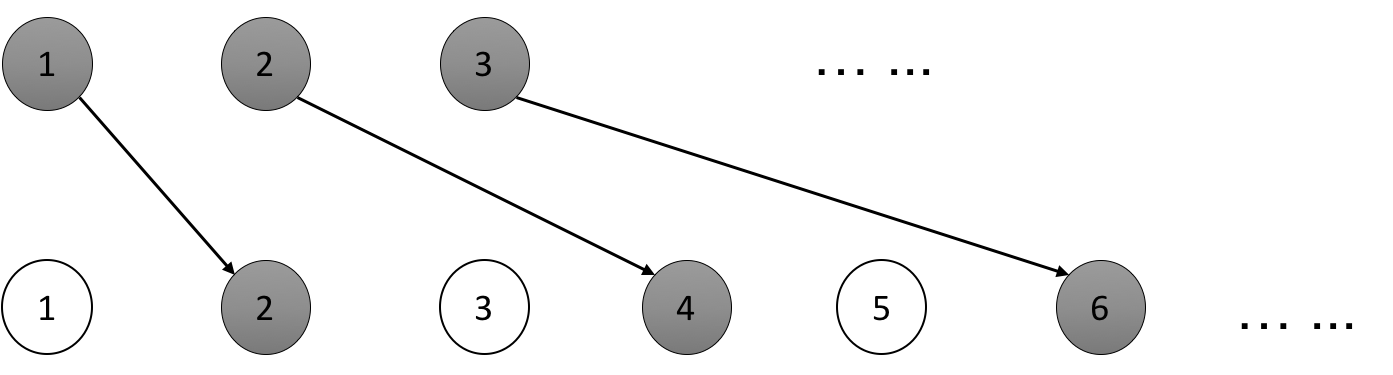
\includegraphics[scale=0.4]{img/Hilbert-hotel-2}
 \caption{希尔伯特无穷旅馆的第二天}
 \label{fig:Hilbert-hotel-2}
\end{figure}

第二天的故事如\cref{fig:Hilbert-hotel-2}所示,我们实际上建立了自然数到偶数间的一一映射,从而空出了无穷多奇数房间,而这些空房间又和旅游团的无穷多位客人之间建立了一一映射,这恰好是奇数到自然数间的一一映射。要想解决希尔伯特旅馆第三天的问题,我们需要在无穷个无穷旅游团和无穷个房间之间建立一一对应。有人说,可以先让第一个旅游团依次入住1, 2, ...号房间,然后让第二个旅游团的第一个客人住在$\infty + 1$号房间,第二个客人住$\infty + 2$号房间……以此类推。但这样的思路行不通。考虑安排客人的过程,第二个旅游团的第一名客人永远不知道第一个旅游团何时入住完,从而确定自己应该搬入的房间。反之,在第一天的故事中,一旦1号房间的客人搬入2号房间,新客人就可以立即入住。尽管每位客人依次搬入下一个房间是一个无穷无尽的过程。第二天的故事也是如此,原1号房间的客人一旦搬到2号房间,旅游团中的第一名客人可以立即搬入空出来的1号房间了,接下来原2号房间的客人搬到4号房间,原3号房间的客人搬到6号房间,此时旅游团中的第2名客人可以立即搬入3号房间了……

\begin{figure}[htbp]
\centering
\begin{tikzpicture}
  \draw[step=1, very thin, gray] (0, 0) grid (5, 5);
  \draw[->] (-0.25, 0) -- (6, 0) coordinate (x axis);
  \draw[->] (0, -0.25) -- (0, 6) coordinate (y axis);
  \foreach \x in {0, 1, 2, 3, 4, 5}
    \path (\x, -0.25) node[left] {\x};
  \foreach \y in {1, 2, 3, 4, 5}
    \path (-0.25, \y) node[below] {\y};
  \foreach \i / \x / \y in {0/0/0, 1/1/0, 2/0/1, 3/0/2, 4/1/1, 5/2/0, 6/3/0, 7/2/1, 8/1/2, 9/0/3, 10/0/4}{
    \path (\x, \y) coordinate (N\i);
    \fill (N\i) circle (1pt) node[above right=3pt of N\i] {\i};
  }
  \foreach \i in {0,...,9} {
    \pgfmathsetmacro{\j}{\i+1}
    \draw[-latex, thick] (N\i) to (N\j);
  }
\end{tikzpicture}
\caption{对无穷个无穷的一种编号方案}
\label{fig:NNtoN}
\end{figure}

\cref{fig:NNtoN}给出了一种编号方案。为了方便,我们让每个旅游团的第一个客人编号为0,第二个客人编号为1,第三个客人编号为2……,我们把已经在旅馆中入住的客人编号为0号旅游团,新来的第一个旅游团编号为1号团,第二个旅游团编号为2号团……在这个图中,每个客人就对应无穷伸展的方格子中的一个点。同样我们让旅馆的房间号也从0开始。现在我们按照这个顺序安排入住:第0号团的第0号客人入住0号房间,第0号团的第1号客人入住1号房间,第1号团的第0号客人入住第2号房间,第2号团的第0号客人入住3号房间,第1号团的第1号客人入住4号房间……这样按照图中往返画“之”字形,就可以逐一、并且毫无遗漏地安排每个客人入住。我们在无穷个旅游团的每个客人和无穷个房间之间建立了一一映射。希尔伯特的旅馆神奇地容纳了“二维”的无穷\footnote{还有一种解法使用了欧几里得证明的素数有无穷多的结论。将酒店中每个奇数房间$i$的客人安排到$2^i$房间去。然后将第一个旅游团的每个客人安排到$3^n$房间去,将第二个旅游团的每个客人安排到$5^n$的房间,...第$k$个旅游观的每个客人安排到$p^n$房间去,其中$p$是第$k$个素数。这一解法的缺点是有些空房间,例如15号,没有客人入住。}。

\begin{Exercise}\label{ex:grand-hotel}
\Question{我们用\cref{fig:NNtoN}建立了房间和任意旅游团的客人间的一一映射。第$i$号旅游团的第$j$号客人应该入住几号房间?第$k$个房间里住了哪号旅游团的哪位客人?}
\Question{希尔伯特旅馆第三天的故事的解法并不唯一,\cref{fig:PWW-NNtoN}是《无需语言的证明》一书的封面。试根据此图给出另一种编号方案?
\begin{figure}[htbp]
 \centering
 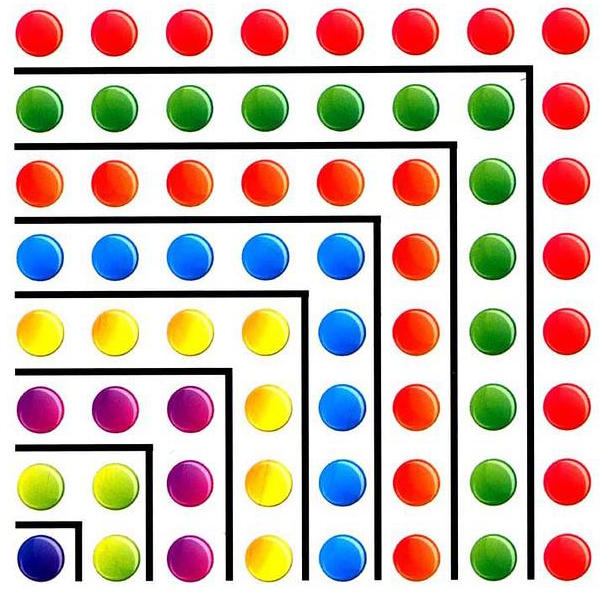
\includegraphics[scale=0.18]{img/PWW}
 \caption{《无需语言的证明》封面局部}
 \label{fig:PWW-NNtoN}
\end{figure}
}
\end{Exercise}

\begin{Answer}[ref = {ex:grand-hotel}]
\Question{我们用\cref{fig:NNtoN}建立了房间和任意旅游团的客人间的一一映射。第$i$号旅游团的第$j$号客人应该入住几号房间?第$k$个房间里住了哪号旅游团的哪位客人?

按照本章约定,从0开始计数。用数偶$(i, j)$表示第$i$号旅游图的第$j$号客人。我们列出前面的几个客人和房间的对应关系

\vspace{3mm}
\begin{adjustbox}{max width=\linewidth}
\begin{tabular}{c|c|c|c|c|c|c|c|c|c|c|c}
$(i, j)$ & (0, 0) & (0, 1) & (1, 0) & (2, 0) & (1, 1) & (0, 2) & (0, 3) & (1, 2) & (2, 1) & (3, 0) & ... \\
\hline
$k$ & 0 & 1 & 2 & 3 & 4 & 5 & 6 & 7 & 8 & 9 & ... \\
\hline
$i + j$ & 0 & 1 & 1 & 2 & 2 & 2 & 3 & 3 & 3 & 3 & ... \\
\end{tabular}
\end{adjustbox}
\vspace{3mm}

如果同时写下$i+j$的值,我们发现规律是很明显的。共有1个0,2个1,3个2,4个3……这些恰恰是毕达哥拉斯发现的三角形数。记$m = i + j$,对于图中任意格点,它表明在这个点的左下方所有斜线上格点的数目为:$\dfrac{m(m + 1)}{2}$。

在这个点所在的斜线上,如果$m$是奇数则向左上前进,$i$增加、$j$减小;如果是偶数则向右下前进。综合起来,我们得到结果:

\[
k = \dfrac{m(m + 1)}{2} + \begin{cases} m - j: \text{$m$是奇数} \\
j: \text{$m$是偶数} \\
\end{cases}
\]

进一步,我们可以通过$(-1)^m$来简化这个结果:

\[
k = \dfrac{m(m + 2) + (-1)^m (2j - m)}{2}
\]
}
\Question{希尔伯特旅馆第三天的故事的解法并不唯一,\cref{fig:PWW-NNtoN}是《无需语言的证明》一书的封面。试根据此图给出另一种编号方案?
\begin{center}
 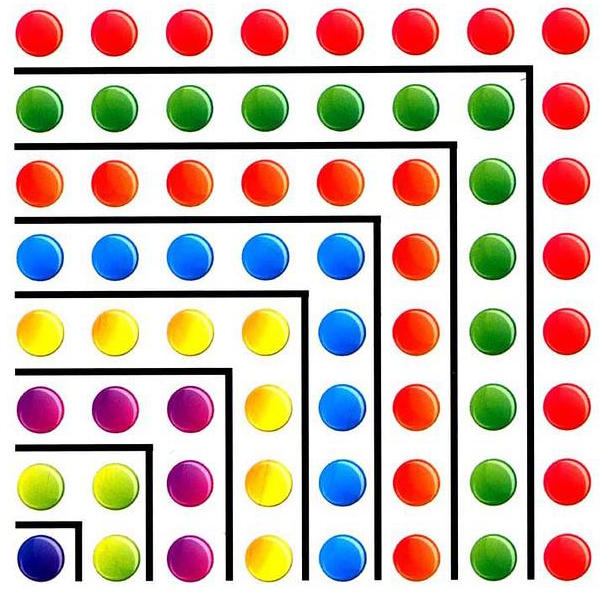
\includegraphics[scale=0.18]{img/PWW}
 \captionof{figure}{《无需语言的证明》封面局部}
\end{center}

\begin{center}
\begin{tikzpicture}
  \draw[step=1, very thin, gray] (0, 0) grid (5, 5);
  \draw[->] (-0.25, 0) -- (6, 0) coordinate (x axis);
  \draw[->] (0, -0.25) -- (0, 6) coordinate (y axis);
  \foreach \x in {0, 1, 2, 3, 4, 5}
    \path (\x, -0.25) node[left] {\x};
  \foreach \y in {1, 2, 3, 4, 5}
    \path (-0.25, \y) node[below] {\y};
  \foreach \i / \x / \y in {0/0/0, 1/1/0, 2/1/1, 3/0/1, 4/0/2, 5/1/2, 6/2/2, 7/2/1, 8/2/0, 9/3/0, 10/3/1}{
    \path (\x, \y) coordinate (N\i);
    \fill (N\i) circle (1pt) node[above right=3pt of N\i] {\i};
  }
  \foreach \i in {0,...,9} {
    \pgfmathsetmacro{\j}{\i+1}
    \draw[-latex, thick] (N\i) to (N\j);
  }
\end{tikzpicture}
\captionof{figure}{对无穷个无穷的另一种编号方案}
\label{fig:NNtoN2}
\end{center}

如\cref{fig:NNtoN2}所示,每次沿着折尺形前进,每个折尺上有奇数个点。
}
\end{Answer}

\subsection{一一对应与无穷集合}

从希尔伯特旅馆的故事中,我们看到一一对应的概念对于研究无穷的重要性。如果能建立两个集合间的一一对应关系,则它们具有相同的基数。进一步我们可以用一一对应对集合进行分类。

%% 我们曾经在第三章介绍过相应的概念。具体说就是在两个集合$A$和$B$之间建立一个映射$A \arrowto{f} B$,使得$A$中的每个元素$x$,都可以通过映射$x \mapsto y = f(x)$,与$B$中的元素$y$关联起来。对于集合,我们也称映射$f$为函数。$y$叫作$x$的像,而$x$叫作原像。如果原像是唯一的,我们称这样的映射为\textbf{单射};如果$B$中的任何$y$都存在原像,我们称这样的映射为\textbf{满射}。既是单射又是满射的映射称为一一映射。\cref{fig:bijection}描述了两个有限集合间的一个一一映射。

%% \begin{figure}[htbp]
%% %\begin{wrapfigure}{R}{0.4\textwidth}
%%  \centering
%%  \includegraphics[scale=0.4]{img/bijection}
%%  %\captionsetup{labelformat=empty}
%%  \caption{集合间的一一对应}
%%  \label{fig:bijection}
%% %\end{wrapfigure}
%% \end{figure}

希尔伯特的无穷旅馆系列故事既让人感到神奇和震惊,也让人困惑。自然数不仅和它的无穷子集奇数和偶数同样多,并且一维的自然数$n$和二维的自然数对$(m, n)$也同样多。这意味着什么呢?康托尔发现,他可以从自然数开始,利用一一对应,扩展出一系列的无穷集合。我们来看一下这些例子。

\begin{enumerate}
\item \textbf{整数}。如果我们建立这样的一一对应:

\begin{tabular}{ccccccccc}
0 & 1 & -1 & 2 & -2 & ... & $n$ & $-n$ & ... \\
$\updownarrow$ & $\updownarrow$ & $\updownarrow$ & $\updownarrow$ & $\updownarrow$ & & $\updownarrow$ & $\updownarrow$ & \\
0 & 1 &  2 & 3 &  4 & ... & $2n - 1$ & $2n$ & ... \\
\end{tabular}

这样就把整数和自然数对应起来。换一种角度,我们实际上用奇数对应了全部正整数,用偶数对应了零和全部负整数。这说明全体整数和自然数一样多。换言之,我们可以用自然数构造整数。
\item \textbf{有理数}。我们知道,有理数又叫作可比数,可以写成$p/q$的形式,其中$q \neq 0$。回想希尔伯特无穷旅馆第三天的的故事,用同样的方法,我们可以在任何数偶$(p, q)$和自然数之间建立一一映射。我们只要稍作修改就可以建立有理数$p/q$和自然数间的一一对应。先不考虑负数的情形,每当遇到第二个数$q$等于0就跳过,如果$p/q$不是既约分数(含有公因子)就跳过。然后我们复用扩展整数的方法,再把负有理数包含进来,这样就从自然数构造出了全体有理数。例如下表给出了前几个自然数到有理数的对应关系:

\begin{tabular}{cccccccccc}
0 & 1 & 2 & 3 & 4 & 5 & 6 & 7 & 8 & ... \\
$\updownarrow$ & $\updownarrow$ & $\updownarrow$ & $\updownarrow$ & $\updownarrow$ & $\updownarrow$ & $\updownarrow$ & $\updownarrow$ & $\updownarrow$ & \\
0 & 1 & $\dfrac{1}{2}$ & $-\dfrac{1}{2}$ & -1 & -2 & $-\dfrac{2}{3}$ & $-\dfrac{1}{3}$ & $\dfrac{1}{3}$ & ... \\
\end{tabular}

这说明自然数和有理数同样多。

\index{代数数}
\item \textbf{代数数}。所谓代数数,是指可以通过代数方程求解出的数。简单说,就是可以通过有限次加减乘除、乘方开方得到的数。因此$\sqrt{2}$和$1 \pm \sqrt{3}i$是代数数,而$\pi, e$都不是代数数。因此,任意给定一个整系数代数方程:
\[
a_0 x^n + a_1 x^{n-1} + ... + a_n = 0
\]
其中$a_0, a_1, ... a_n$都是整数,且$a_0 \neq 0$。它的所有根都是代数数。我们构造一个正整数:
\[
h = n + |a_0| + |a_1| + ... + |a_n|
\]
也就是次数和方程系数绝对值的和。我们称$h$为方程的高。因此,对于任意的代数方程,高$h$总是一个确定的自然数。反之,给定一个自然数$h$,对应的方程却不止一个。例如:$x - 3 = 0, x^3 + 1 = 0, x^3 - 1 = 0, x^2 + x + 1 = 0, x^2 - x + 1 = 0$的高都是4。但是对于固定的$h$,以它为高的代数方程只有有限多个。因此我们可以把所有的代数方程枚举出来,先枚举$h=1$的代数方程,再枚举$h=2$的代数方程……如此下去,就可以把所有的代数方程都枚举出来。当然,高同样的方程可以按任意顺序排列。根据高斯证明的代数基本定理,方程根的个数等于它的次数$n$。如果考虑重根,则不同的根不超过$n$。于是高为$h$的代数方程的根只有有限个。现在我们就可以枚举所有代数数了。

首先把高$h=1$的代数方程(只有一个$x = 0$)的根枚举出,就是0,再把高为2的方程的所有根枚举出。注意,不同方程的某个根可能是相等的,如果我们遇到某个根,在此前已经枚举过了,我们就将它跳过。这样就把代数数同自然数一一对应起来了。因此,自然数和代数数同样多。换言之,我们可以通过自然数扩展出全部代数数。
\end{enumerate}

接下来我们遇到了难题,我们能否从自然数扩展到实数?不仅包括普通的无理数,还包括$\pi$,$e$这样的超越数?解决这个难题的是康托尔和戴德金。在进一步介绍这些伟大的成果之前,让我们先了解一下这两位数学家。


\begin{figure}[htbp]
 \centering
 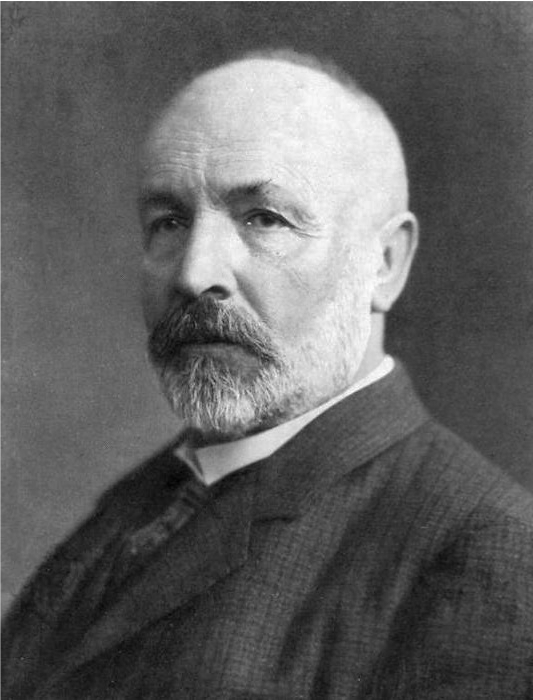
\includegraphics[scale=0.5]{img/Cantor}
 \caption{格奥尔格·康托尔(1845-1918)}
 \label{fig:Cantor}
\end{figure}

\begin{mdframed}
\index{康托尔}
康托尔是德国数学家,集合论的创始人。1845年3月3日生于俄罗斯圣彼得堡,他一生的大部分时间是在德国度过的。康托尔的父亲是具有犹太血统的丹麦商人,母亲出身艺术世家。1856年举家迁居德国的法兰克福。尽管康托尔较早就显示出了数学才能,他的父亲却希望他成为一名工程师,因为这样更容易求职和谋生。直到17岁时,康托尔的父亲才逐渐意识到不应该把自己的意见强加给儿子。他得到父亲的允许,进入大学学习数学。康托尔给父亲回信道:“你自己也能体会到你的信使我多么高兴。这封信确定了我的未来……现在我很幸福,因为我看到如果我按照自己的感情选择,不会使你不高兴。我希望你能活到在我身上找到乐趣,亲爱的父亲;从此以后我的灵魂,我整个人,都为我的天职活着;一个人渴望做什么,凡是他的内心强制他去做的,他都会成功!”\cite{HanXueTao16}

1862年,康托尔进入苏黎世大学,1863年转入柏林大学攻读数学和神学,受教于大数学家库默尔、魏尔斯特拉斯、和克罗内克。1866年曾去哥廷根学习一个学期。1867年他在库默尔的指导下以解决整系数不定方程的论文获得博士学位。当时的数学界正在魏尔斯特拉斯的领导下进行着重建微积分严密基础的运动,康托尔也很快转入这一研究方向。在工作中,他意识到必须研究作为微积分基础的实数点集,这成为了集合论研究的开端。

1872年康托尔在瑞士旅游中偶遇了数学家戴德金。两人后来成为亲密的朋友,彼此通过信件交流,互相支持。1874年29岁的康托尔发表了关于集合论的第一篇革命性论文。康托尔开始显示他非凡的独创力。在随后的十几年中,他几乎独自一人把集合论推向深入,引领了数学中无穷的革命。在他最伟大的、最具创见的时期,康托尔却没有能得到应有的认可。他没能取得柏林大学的教授职位。他的大部分研究时光是在哈雷大学度过的。这是一所不大出名、薪金微薄的二流学院。他的成果在当时很难被理解。由于太过颠覆传统,加之无穷集合引发了一些悖论(我们将在下一章详细介绍罗素悖论),人们对集合论的基础和可靠性产生了严重的怀疑。康托尔遭到了许多人的反对,其中反对最激烈的是他的老师,柏林学派的代表人物克罗内克。克罗内克有一句名言:“上帝创造了自然数,其余都是人的工作。”他批判康托尔的无穷集合和超限数理论不是数学而是神秘主义,是一类危险的数学疯狂。他认为数学在康托尔的领导下正在走向疯人院。除了克罗内克之外,还有一些著名的数学家也对集合论发表了反对意见,包括法国著名数学家——被称为最后一个数学通才的庞加莱,他说:“我个人,而且还不只我一个人,认为重点在于,切勿引进一些不能用有限个文字去完全定义好的东西。”他把集合论当作一个有趣的“病理学的情形”来谈,并且预测说:“后一代将把集合论当作一种疾病,而人们已经从中恢复过来了”。德国数学家赫尔曼$\cdot$外尔认为,康托尔关于基数的等级观点是“雾上之雾”。克莱因也不赞成集合论的思想。施瓦兹原来是康托尔的好友,但他由于反对集合论而同康托尔断交。集合论的悖论出现之后,一些数学家开始认为集合论根本是一种病态,他们以不同的方式发展为经验主义、直觉主义、构造主义等学派,在数学的基础大战中,构成反康托尔的阵营。

于是悲剧的结局不是集合论进入了疯人院,而是康托尔进入了疯人院。1884年5月,他支持不住了,第一次精神崩溃。在他一生的随后岁月中,这种崩溃以不同强度反复发生,把他从社会上赶进精神病院这个避难所。1904年在两个女儿的陪同下,他出席了第三届国际数学家大会。会上他的精神受到严重刺激,立即被送进医院。在他生命的最后十年,他大都处于严重的抑郁状态中,并在哈雷大学的精神病诊所度过了漫长的岁月。他最后一次住进精神病院是1917年5月,直至1918年1月去世。

康托尔的集合论得到公开的承认和热情的称赞应该说首先在瑞士苏黎世召开的第一届国际数学家大会上表现出来。瑞士苏黎世理工大学教授胡尔维茨(Hurwitz,Adolf,1859-1919)在他的综合报告中,明确地阐述康托尔集合论对函数论的进展所起的巨大推动作用,这破天荒第一次向国际数学界显示康托尔的集合论不是可有可无的哲学,而是真正对数学发展起作用的理论工具。在分组会上,法国数学家阿达玛也报告康托尔对他的工作的重要作用。随着时间的推移,人们逐渐认识到集合论的重要性。希尔伯特高度赞誉康托尔的集合论“是数学天才最优秀的作品”,“是人类纯粹智力活动的最高成就之一”,“是这个时代所能夸耀的最巨大的工作”。在1900年第二届国际数学家大会上,希尔伯特高度评价了康托尔工作的重要性,并把康托尔的连续统假设列入20世纪初有待解决的23个重要数学问题之首。当康托尔的朴素集合论出现一系列悖论时,直觉主义学派的代表布劳威尔等人借此再次发难,希尔伯特用坚定的语言向他的同代人宣布:“没有任何人能将我们从康托尔所创造的伊甸园中驱赶出来”。
\end{mdframed}

\subsection{可数无穷与不可数无穷}
\index{可数集}
迄今为止,我们用自然数构造了整数、有理数、包含部分无理数的代数数。它们都和自然数之间存在一一映射,或者说和自然数一样多。我们把和自然数等势的无穷集合叫作可数无穷。是不是所有的无穷集合都是可数的呢?是否存在更大的无穷呢?1873年11月29日康托尔给戴德金的一封信中提到了这个问题:“取所有的自然数集合,记为$N$,然后考虑所有实数的集合,记为$R$。简单来说,问题就是两者是否能够对应起来,使得一个集中的每一个体只对应另一集中一个唯一的个体?乍一看,我们可以说答案是否定的,这种对应不可能,因为前者由离散的部分组成,而后者则构成一个连续统。但从这种说法里我们什么也得不到。虽然我非常倾向认为这两者不能有这样的一个一一对应,但是我找不出理由,我对这事极为关注,也许这理由非常简单。”

\index{对角线证明}
一个星期后的12月7日,在写给戴德金的信中,康托尔自己回答了这个问题,他发现实数集合不能和自然数集合构成一一对应。这一天可以看作是集合论的诞生日。康托尔曾经给出过两个证明,其中第二个证明最为脍炙人口,就是大名鼎鼎的“对角线证明”。

康托尔首先使用反证法,假设区间$(0, 1)$上的全部实数是可数的,可以和自然数一一对应。那么就可以把这个区间里的全部实数列出来,形成一个序列$a_0, a_1, a_2, ..., a_n, ...$。现在将这个序列中的每个实数都表示成小数形式。如果是无理数,它的小数形式是无限不循环的;如果是除不尽的分数,则其小数形式是无限循环的,例如$\dfrac{1}{3} = 0.333...$;如果能够除尽,我们就在后面补无穷多个零,例如$\dfrac{1}{2} = 0.5000...$。于是实数区间$(0, 1)$中的所有实数可以排成下面的序列:

\[
\begin{array}{l}
a_0 = 0.a_{00}a_{01}a_{02}a_{03}...\\
a_1 = 0.a_{10}a_{11}a_{12}a_{13}...\\
a_2 = 0.a_{20}a_{21}a_{22}a_{23}...\\
a_3 = 0.a_{30}a_{31}a_{32}a_{33}...\\
... \\
a_n = 0.a_{n0}a_{n1}a_{n2}a_{n3}...\\
... \\
\end{array}
\]

有一点我要提醒一下读者:$a_0, a_1, a_2, ...$并不一定是按照大小次序排列的。现在构造一个数$b = 0.b_0b_1b_2b_3...b_n...$,使它的第$n$位数字$b_n \neq a_{nn}$。为了做到这一点,我们可以规定一个很简单的规则,例如若$a_{nn} \neq 5$,就让$b_n = 5$,否则就让$b_n = 6$,即:

\[
b_n = \begin{cases}
5 & : a_{nn} \neq 5 \\
6 & : a_{nn} = 5 \\
\end{cases}
\]

这样构造出来的数$b$一定不等于上述序列中的任何一个数。因为至少它们的第$n$位数字不相同。也就是对角线上的数字至少不同。我们把对角线上的数字写成黑体,这样就很明显了。

\[
\begin{array}{l}
a_0 = 0.\pmb{a_{00}}a_{01}a_{02}a_{03}...\\
a_1 = 0.a_{10}\pmb{a_{11}}a_{12}a_{13}...\\
a_2 = 0.a_{20}a_{21}\pmb{a_{22}}a_{23}...\\
a_3 = 0.a_{30}a_{31}a_{32}\pmb{a_{33}}...\\
... \\
a_n = 0.a_{n0}a_{n1}a_{n2}a_{n3}...\pmb{a_{nn}}...\\
... \\
\end{array}
\]

我们此前假设$(0, 1)$间的所有实数都被逐一列出了,无一遗漏。$b$显然属于这一区间,但它却不等于任何一个$a_i$。这说明我们假设的一一映射遗漏了$b$,导致了矛盾,所以假设不成立,我们无法把这一区间的所有实数和自然数之间构造一一映射。由于利用了对角线上的数字都不相等的这一事实,这一证法称作康托尔对角线证明。

有人说,把$b$加进$a_0, a_1, a_2, ...$中去不就可以了么?假设$b$加进去后,处于第$m$个位置,我们仍然可以再次构造一个新数$c$,只要让它的第$m$位不等于$b_m$就又出现了一个没有包含的数。

\index{不可数集}
这一证明简单、直观。它揭示了一个惊人的事实:$(0, 1)$间的实数集是不可数的!它是我们发现的第一个比自然数集更大的无穷集合\footnote{柯朗和罗宾在《什么是数学》中给出了一个更为直观的几何证明。假设单位线段(0, 1)之间的点能排成可数的序列$a_1, a_2, a_3, ...$我们用一个长1/10的区间盖住$a_1$点,用长1/100的区间盖住$a_2$点……用长$1/10^n$的区间盖住$a_n$点,如此下去,则(0, 1)这一单位线段将完全被长为1/10, 1/100, 1/1000……的子区间(可能相互重叠)完全盖住。但这些子区间的长度总和为等比数列$1/10 + 1/100 + 1/1000 + ... = 1/9 < 1$,让总长度为1/9的区间覆盖长度为1的线段是不可能的。所以假设错误,线段上的点是不可数的\cite{Courant1969}。}。接下来,我们构造一个一一映射:$y = \pi x - \dfrac{\pi}{2}$。它把区间$(0, 1)$中的每个实数,映射到区间$(-\dfrac{\pi}{2}, \dfrac{\pi}{2})$中,无一遗漏。因此我们立即得知这一区间内的实数集是不可数的。接下来,我们压上最后一根稻草。再构造一个一一映射:$ y = tan(x)$。它把区间$-\dfrac{\pi}{2}$到$\dfrac{\pi}{2}$中的每一个实数,无一遗漏地映射到了全体实数集上\footnote{还有一种几何方法可以将单位线段一一映射到全体实数上。我们将单位线段弄弯成为长度为1的半圆弧,然后在圆外画一条无限长的直线L。现在从圆心到L上任意一点P的连线必然与圆弧相交于一点Q。这样就形成了一一映射,如\cref{fig:seg-to-line}。}。康托尔得到了他的重要结论:实数集不再是可数集,它是比可数集更高等级的无穷。康托尔称之为不可数集,记作$C$。

\begin{figure}[htbp]
 \centering
 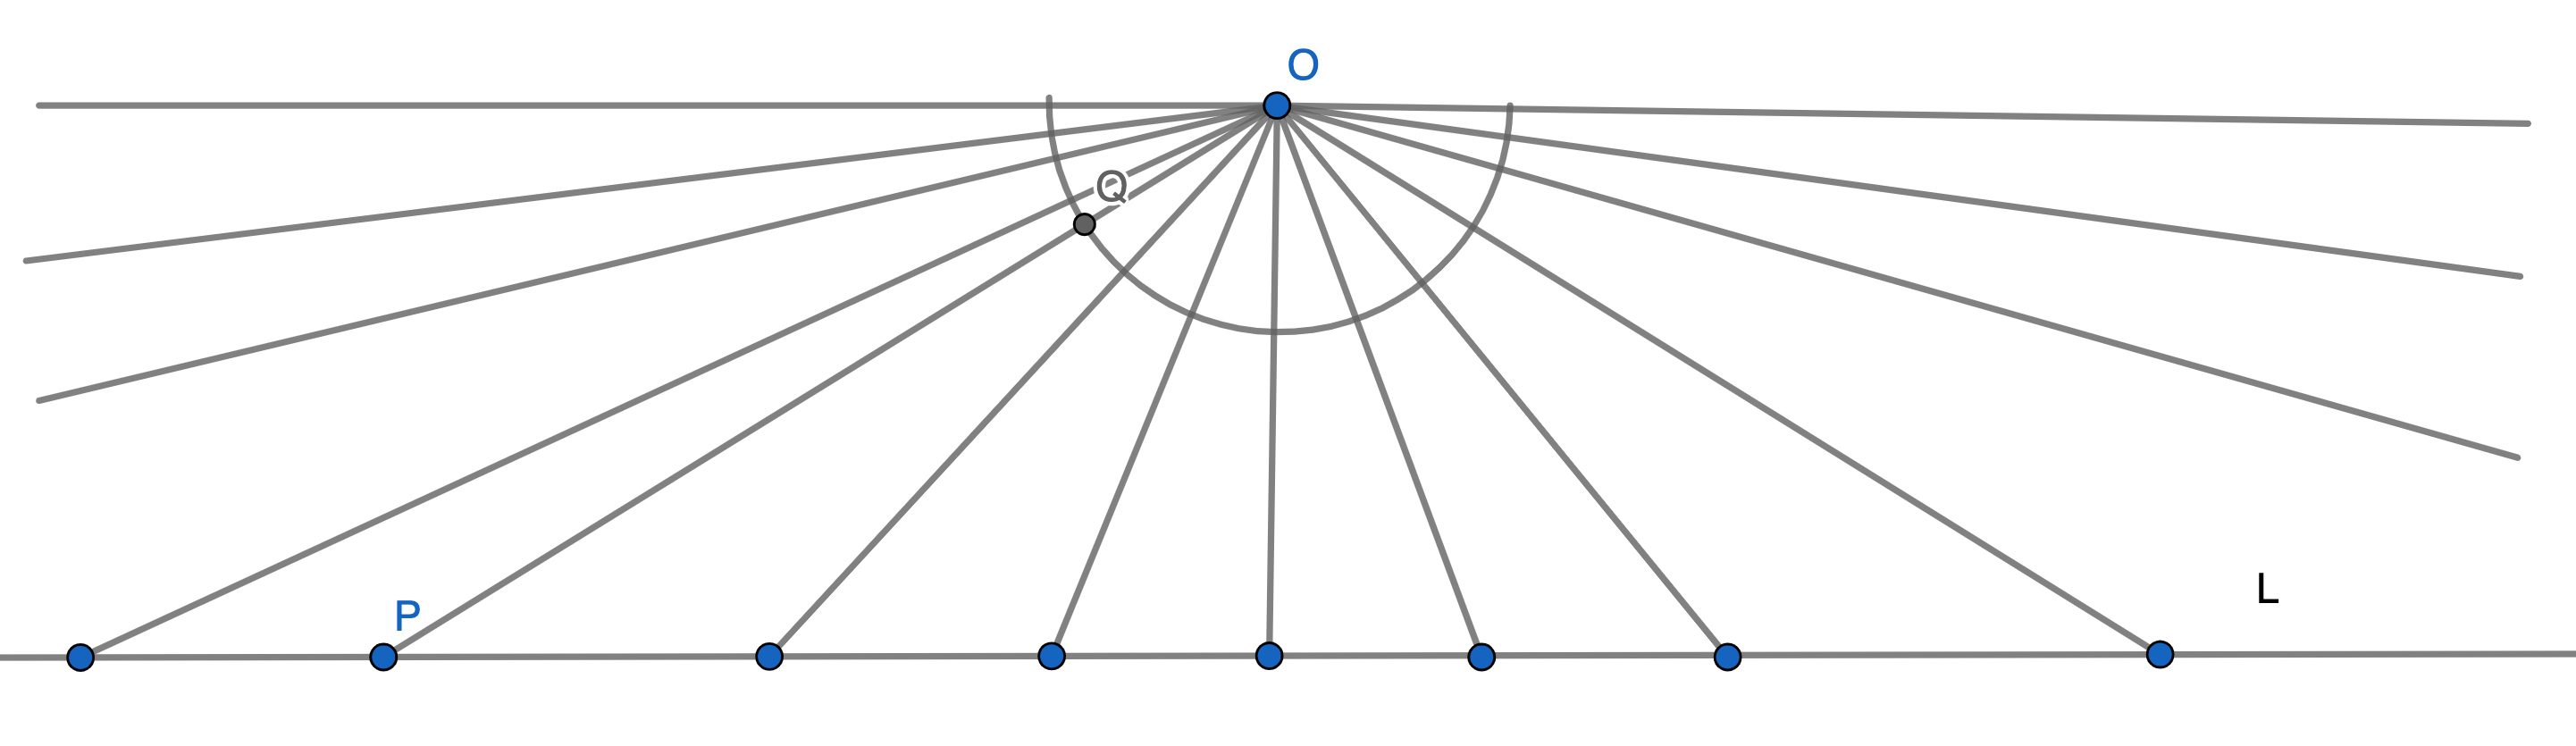
\includegraphics[scale=0.6]{img/seg-to-line}
 \caption{将长度为1的半圆弧映射到实数轴}
 \label{fig:seg-to-line}
\end{figure}

这自然让人联想到线段上的点。在欧几里得的《几何原本》中,点被定义为没有大小的部分,而直线被认为由点组成。根据希帕索斯的发现,我们知道直线上存在无理数。或者说有理数不能够填充直线。而实数是可以填充线段的。我们在下一节中,还会介绍戴德金分割,从而给出实数的严密化定义。上面的证明告诉我们,单位长度线段上的点,和任何长度线段上的点,以及无限长的直线上的点,也就是数轴上稠密的点是一样多的。都是不可数集。同心圆上的点也是同样多的,它们也都是不可数集。

同样令人吃惊的是无理数与有理数多少的比较。直观上思考,任何两个有理数之间,存在着无穷多的无理数;任何两个无理数之间,也存在着无穷多的有理数,我们会觉得无理数和有理数应该一样多。然而康托尔的结论告诉我们,有理数是可数的,而无理数是不可数的。这说明无理数远远多于有理数。再进一步,我们前面证明了代数数是可数的,这说明像$\pi, e$这样的超越数是不可数的,它们要远远多于代数数。


\begin{Exercise}[label={ex:algebraic}]
\Question{假设$x^n + y^n = z^n$,证明若$x, y, z$任何两个含有公约数$d$,则第三个也有这个因子。\label{qn:xyz-coprime}}

\Question{证明若首一代数方程$x^n + a_{n-1} x^{n-1} + \dotsb + a_1 x + a_0 = 0$存在有理解,则这个解必定是整数。 \label{qn:rational-solution-is-integral}}

\Question{证明范数是可乘的。\label{qn:norm-is-multiplicative}}

\Question{说明二次整数范数是对应二次方程的常数项。\label{qn:quadratic-norm}}

\Question{如果$a, b$互素,证明共轭的二次整数$a \pm bi\sqrt{m}$互素。\label{qn:coprime-of-conjugates}}

\Question{从范数的共轭定义说明爱森斯坦整数的范数为$a^2 - ab + b^2$。\label{qn:norm-of-z-omega}}

\Question{证明爱森斯坦整数的范数非负。}

\Question{爱森斯坦整数中的单位元是什么?}

\Question{试画出爱森斯坦整数$\rho \beta$的格点。}

\Question{根据爱森斯坦整数的格点,证明欧几里得算法存在。}

\Question{证明$1 \pm i\sqrt{5}$是不可分解的。\label{qn:1-n-delta-irreducible}}

\Question{证明理想的和仍是理想。\label{qn:sum-of-ideals}}

\Question{(0)叫做零理想,(1)叫做单位理想。它们各自包含了什么元素?\label{qn:trivial-ideals}}

\Question{验证如果理想$A = (a, b) = \{ax + by | x, y \in R\}$,理想$B = (c, d)$,则$AB = (ac, ad, bc, bd)$。\label{qn:ideal-product}}

\Question{*试用理想解决$4 = 2 \times 2 = (1 + i\sqrt{3})(1 - i\sqrt{3})$的唯一分解。}

\end{Exercise}

\begin{Answer}[ref={ex:algebraic}]
\Question{假设$x^n + y^n = z^n$,证明若$x, y, z$任何两个含有公约数$d$,则第三个也有这个因子。}

\Question{证明若首一代数方程$x^n + a_{n-1} x^{n-1} + \dotsb + a_1 x + a_0 = 0$存在有理解,则这个解必定是整数。}

\Question{证明范数是可乘的。

利用共轭复数的可乘性。
}

\Question{说明二次整数范数是对应二次方程的常数项。

韦达定理
}

\Question{如果$a, b$互素,证明共轭的二次整数$a \pm bi\sqrt{m}$互素。

let $d = (a, b), z = a + bi\sqrt{m}, d | z \pm \overline{z}$ this gives $d | 2a, d | 2bi\sqrt{m}$. But $d$ can't be 2, or $a, b$ both are even; hence $d$ divides both $a, b$, which must be 1.
}

\Question{从范数的共轭定义说明爱森斯坦整数的范数为$a^2 - ab + b^2$。}

\Question{证明爱森斯坦整数的范数非负。}

\Question{爱森斯坦整数中的单位元是什么?}

\Question{试画出爱森斯坦整数$\rho \beta$的格点。}

\Question{根据爱森斯坦整数的格点,证明欧几里得算法存在。}

\Question{证明$1 \pm i\sqrt{5}$是不可分解的。

\begin{proof}
假设它可以分解为$(a + bi\sqrt{5})(c + di\sqrt{5})$,两边取范数:

\[
6 = 1^2 + 5^2 = N(1 \pm i\sqrt{5}) = N(a + bi\sqrt{5})N(c + di\sqrt{5}) = (a^2 + 5b^2)(c^2 + 5d^2)
\]

可以排除掉$a^2 + 5b^2 = 2, c^2 + 5d^2 = 3$的情况,此时$a, b, c, d$没有整数解。只能是$a^2 + 5b^2 = 1$或$c^2 + 5d^2 = 1$。范数为1对应单位元,另一个是相伴元。因此$1 \pm i\sqrt{5}$不可分解。
\end{proof}
}

\Question{证明理想的和仍是理想。\label{qn:sum-of-ideals}}

\Question{(0)叫做零理想,(1)叫做单位理想。它们各自包含了什么元素?\label{qn:trivial-ideals}}

\Question{验证如果理想$A$由$(a, b)$产生,理想$B$由$(c, d)$产生,则$AB = (ac, ad, bc, bd)$。

}

\Question{*试用理想解决$4 = 2 \times 2 = (1 + i\sqrt{3})(1 - i\sqrt{3})$的唯一分解。}
\end{Answer}

\ifx\wholebook\relax \else
\section{参考答案}
\shipoutAnswer

\subimport{inc/}{fibonacci-zh-cn}
\subimport{inc/}{wilson-zh-cn}

\begin{thebibliography}{99}
\subimport{inc/}{bib-zh-cn}
\end{thebibliography}

\expandafter\enddocument
\fi
